\documentclass[11pt]{article}
\usepackage{minted}
\usepackage{amsmath,amsthm,amsfonts,amssymb,amscd}
\usepackage{multirow,booktabs}
\usepackage[table]{xcolor}
\usepackage{fullpage}
\usepackage{lastpage}
\usepackage{enumitem}
\usepackage{fancyhdr}
\usepackage{mathrsfs}
\usepackage{wrapfig}
\usepackage{setspace}
\usepackage{calc}
\usepackage{multicol}
\usepackage{cancel}
\usepackage[retainorgcmds]{IEEEtrantools}
\usepackage[margin=3cm]{geometry}
\usepackage{amsmath}

\usepackage{soul} % strikethru

% Tikz arrows to point at equations
\usepackage{tikz}
\usepackage[outline]{contour} % glow around text
\usetikzlibrary{arrows,arrows.meta}
\usetikzlibrary{decorations.markings}
\tikzset{>=latex} % for LaTeX arrow head
\usepackage{xcolor}
\colorlet{Icol}{blue!50!black}
\colorlet{Ccol}{orange!90!black}
\colorlet{Rcol}{green!50!black}
\colorlet{loopcol}{red!90!black!25}
\colorlet{pluscol}{red!60!black}
\colorlet{minuscol}{blue!60!black}
\newcommand\EMF{\mathcal{E}} %\varepsilon}
\contourlength{1.5pt}
\tikzstyle{EMF}=[battery1,l=$x(t)$,invert]
\tikzstyle{internal R}=[R,color=Rcol,Rcol,l=$r$,/tikz/circuitikz/bipoles/length=30pt]
\tikzstyle{loop}=[->,red!90!black!25]
\tikzstyle{loop label}=[loopcol,fill=white,scale=0.8,inner sep=1]
\tikzstyle{thick R}=[R,color=Rcol,thick,Rcol,l=$R$]
\tikzstyle{thick C}=[C,thick,color=Ccol,Ccol,l=$C$]
\tikzstyle{myswitch}=[closing switch,line width=0.3] %-{Latex[length=3]},

\newcommand{\myvoltmeter}[2] 
{  % #1 = name , #2 = rotation angle
  \begin{scope}[transform shape,rotate=#2]
  \draw[thick] (#1)node(){$\mathbf V$} circle (11pt);
  \draw[rotate=45,-latex] (#1)  +(-17pt,0) --+(17pt,0);
  \end{scope}
}
\usetikzlibrary{tikzmark}

\newlength{\tabcont}
\setlength{\parindent}{0.0in}
\setlength{\parskip}{0.05in}
\usepackage{empheq}
\usepackage{framed}
\usepackage[most]{tcolorbox}
\usepackage{xcolor}
\colorlet{shadecolor}{orange!15}
\parindent 0in
\parskip 12pt
\geometry{margin=1in, headsep=0.25in}
\usepackage{hyperref}
\hypersetup{
    colorlinks=true,
    linkcolor=blue,
    filecolor=blue,
    urlcolor=cyan,
}
% To make " match
\usepackage[english]{babel}
\usepackage[autostyle, english = american]{csquotes}
\MakeOuterQuote{"}
% For easy derivatives without the \frac{\mathrm{d}^2 \omega}{\mathrm{d}\theta^2}
\usepackage[thinc]{esdiff} % ex: \diff{f}{x} &\qquad \diff*[4]{g}{t}{t = 1}
\usepackage{tikz}
\usetikzlibrary{positioning}

\usepackage{enumitem} % http://ctan.org/pkg/enumitem
\setlist{nosep}
\setlist[itemize]{topsep=-0.1cm}

% \usepackage{physics} % for derivatives, (e.g. \dv, \pdv)
\usepackage[siunitx]{circuitikz} %[symbols]


\def\P{\mathbb{P}} % Probability
\def\d{\mathrm{d}}
\def\zt{\stackrel{\mathcal{Z}}{\leftrightarrow}}
\def\ft{\stackrel{\mathcal{F}}{\leftrightarrow}}
\def\Xhat{\hat{X}(z)}
\def\Yhat{\hat{Y}(z)}
\def\Xhatu{\hat{x}(z)}
\def\Yhatu{\hat{y}(z)}
\def\Hhat{\hat{H}(z)}
\def\zinv{z^{-1}}
\def\zn{z^{-n}}
\def\zpn{z^{n}}
\def\zl{z^{-\ell}}
\def\zpl{z^{\ell}}
\def\zN{z^{-N}}
\def\zpN{z^{N}}
\def\zopn{z_{0}^{n}}

\newcommand{\ze}[1]{z^{-#1}}
\newcommand{\Xshat}[1]{\hat{X}_{\text{#1}}(z)}
\newcommand{\Xphat}[1]{\hat{X}\left(#1\right)}
\newcommand{\Hphat}[1]{\hat{H}\left(#1\right)}
\newcommand{\pd}[2]{\frac{\partial{#1}}{\partial{#2}}}
\newcommand{\dv}[2]{\frac{\mathrm d{#1}}{\mathrm d{#2}}}
\newcommand{\pdv}[2]{\frac{\partial{#1}}{\partial{#2}}}
\let\originalmiddle=\middle
\DeclareMathOperator{\sgn}{sgn}

% code
\usepackage{listings}
\usepackage{color}

\usepackage{makecell}


\definecolor{dkgreen}{rgb}{0,0.6,0}
\definecolor{gray}{rgb}{0.5,0.5,0.5}
\definecolor{mauve}{rgb}{0.58,0,0.82}

\lstset{frame=tb,
  language=Java,
  aboveskip=3mm,
  belowskip=3mm,
  showstringspaces=false,
  columns=flexible,
  basicstyle={\small\ttfamily},
  numbers=none,
  numberstyle=\tiny\color{gray},
  keywordstyle=\color{blue},
  commentstyle=\color{dkgreen},
  stringstyle=\color{mauve},
  breaklines=true,
  breakatwhitespace=true,
  tabsize=3
}
% 

\makeatletter
\pgfkeys{/pgf/grid lines/.initial=2}

\pgfdeclareshape{grid}{
    % inherit most things from the rectangle shape
    \inheritsavedanchors[from=rectangle]
    \inheritanchorborder[from=rectangle]
    \inheritanchor[from=rectangle]{center}
    \inheritanchor[from=rectangle]{north}
    \inheritanchor[from=rectangle]{south}
    \inheritanchor[from=rectangle]{west}
    \inheritanchor[from=rectangle]{east}
    \inheritanchor[from=rectangle]{south east}
    \inheritanchor[from=rectangle]{south west}
    \inheritanchor[from=rectangle]{north east}
    \inheritanchor[from=rectangle]{north west}
    \inheritbackgroundpath[from=rectangle]

    \savedmacro\lines{%
        \pgfmathtruncatemacro\lines{\pgfkeysvalueof{/pgf/grid lines}}%
    }

    % draw the grid
    \beforebackgroundpath{
        % store lower right in xa/ya and upper right in xb/yb
        \southwest \pgf@xa=\pgf@x \pgf@ya=\pgf@y
        \northeast \pgf@xb=\pgf@x \pgf@yb=\pgf@y

        % compute distance between the lines
        \pgfmathparse{(\the\pgf@xb-\the\pgf@xa)/(\lines + 1)}
        \pgf@xc=\pgfmathresult pt
        \pgfmathparse{(\the\pgf@yb-\the\pgf@ya)/(\lines + 1)}
        \pgf@yc=\pgfmathresult pt

        % draw grid
        \c@pgf@counta=0
        \c@pgf@countb\lines\relax
        \pgf@xb=\pgf@xa
        \advance\pgf@xb\pgf@xc\relax
        \pgfmathloop
            \ifnum\c@pgf@counta<\c@pgf@countb
                \pgfpathmoveto{\pgfpoint{\pgf@xb}{\pgf@ya}}
                \pgfpathlineto{\pgfpoint{\pgf@xb}{\pgf@yb}}
                \advance\c@pgf@counta 1\relax
                \advance\pgf@xb\pgf@xc\relax
        \repeatpgfmathloop
        % set \pgf@xb to the right side
        \c@pgf@counta=0
        \pgf@yb=\pgf@ya
        \advance\pgf@yb\pgf@yc\relax
        \pgfmathloop
            \ifnum\c@pgf@counta<\c@pgf@countb
                \pgfpathmoveto{\pgfpoint{\pgf@xa}{\pgf@yb}}
                \pgfpathlineto{\pgfpoint{\pgf@xb}{\pgf@yb}}
                \advance\c@pgf@counta 1\relax
                \advance\pgf@yb\pgf@yc\relax
        \repeatpgfmathloop
        \pgfusepath{stroke}
    }

    % add anchors for vertices (intersections of grid lines)
    % and center points (centers of the small rectangles).
    %
    % vertex anchors are simply called 'x y' with '0 0' being the lower left
    % vertex.
    % center anchors are called 'center x y' with 'center 1 1' being the center
    % of the lower left rectangle
    \pgfutil@g@addto@macro\pgf@sh@s@grid{%
        \c@pgf@counta\lines
        \advance\c@pgf@counta 1\relax
        \pgfmathloop\ifnum\c@pgf@counta>-1
            {% group to allow nesting of loops
                \c@pgf@countb\lines
                \advance\c@pgf@countb 1\relax
                \pgfmathloop\ifnum\c@pgf@countb>-1
                    \pgfutil@ifundefined{pgf@anchor@grid@\the\c@pgf@counta\space\the\c@pgf@countb}{%
                        % need to use xdef, so that \c@pgf@counta/b are expanded
                        % vertices
                        \expandafter\xdef\csname pgf@anchor@grid@\the\c@pgf@counta\space\the\c@pgf@countb\endcsname{%
                            \noexpand\southwest \noexpand\pgf@xa=\noexpand\pgf@x \noexpand\pgf@ya=\noexpand\pgf@y
                            \noexpand\northeast \noexpand\pgf@xb=\noexpand\pgf@x \noexpand\pgf@yb=\noexpand\pgf@y
                            \noexpand\pgfmathparse{(\noexpand\the\noexpand\pgf@xb-\noexpand\the\noexpand\pgf@xa)/(\noexpand\lines + 1)*\the\c@pgf@counta}
                            \noexpand\pgf@x=\noexpand\pgf@xa\noexpand\relax
                            \noexpand\advance\noexpand\pgf@x\noexpand\pgfmathresult pt\noexpand\relax
                            \noexpand\pgfmathparse{(\noexpand\the\noexpand\pgf@yb-\noexpand\the\noexpand\pgf@ya)/(\noexpand\lines + 1)*\the\c@pgf@countb}
                            \noexpand\pgf@y=\noexpand\pgf@ya\noexpand\relax
                            \noexpand\advance\noexpand\pgf@y\noexpand\pgfmathresult pt\noexpand\relax
                        }
                        % centers
                        \expandafter\xdef\csname pgf@anchor@grid@center\space\the\c@pgf@counta\space\the\c@pgf@countb\endcsname{%
                            \noexpand\southwest \noexpand\pgf@xa=\noexpand\pgf@x \noexpand\pgf@ya=\noexpand\pgf@y
                            \noexpand\northeast \noexpand\pgf@xb=\noexpand\pgf@x \noexpand\pgf@yb=\noexpand\pgf@y
                            \noexpand\pgfmathparse{(\noexpand\the\noexpand\pgf@xb-\noexpand\the\noexpand\pgf@xa)/(2*(\noexpand\lines + 1))*(2*\the\c@pgf@counta-1)}
                            \noexpand\pgf@x=\noexpand\pgf@xa\noexpand\relax
                            \noexpand\advance\noexpand\pgf@x\noexpand\pgfmathresult pt\noexpand\relax
                            \noexpand\pgfmathparse{(\noexpand\the\noexpand\pgf@yb-\noexpand\the\noexpand\pgf@ya)/(2*(\noexpand\lines + 1))*(2*\the\c@pgf@countb-1)}
                            \noexpand\pgf@y=\noexpand\pgf@ya\noexpand\relax
                            \noexpand\advance\noexpand\pgf@y\noexpand\pgfmathresult pt\noexpand\relax
                        }
                    }{\c@pgf@countb0\relax}
                    \advance\c@pgf@countb-1\relax
                \repeatpgfmathloop
            }
            \advance\c@pgf@counta-1\relax
        \repeatpgfmathloop
    }
}
\makeatother

\theoremstyle{definition}
\newtheorem{defn}{Definition}
\newtheorem{reg}{Rule}
\newtheorem{exer}{Exercise}
\newtheorem{note}{Note}

% imp box
\usepackage{xcolor,mdframed}
\newenvironment{important}[1][]{%
   \begin{mdframed}[%
      backgroundcolor={red!15}, hidealllines=true,
      skipabove=0.7\baselineskip, skipbelow=0.7\baselineskip,
      splitbottomskip=2pt, splittopskip=4pt, #1]%
   \makebox[0pt]{% ignore the withd of !
      \smash{% ignor the height of !
         \fontsize{32pt}{32pt}\selectfont% make the ! bigger
         \hspace*{-19pt}% move ! to the left
         \raisebox{-2pt}{% move ! up a little
            {\color{red!70!black}\sffamily\bfseries !}% type the bold red !
         }%
      }%
   }%
}{\end{mdframed}}
% imp box

\begin{document}
% \setcounter{section}{8}
    \title{EE 120 Lecture Notes}
    
    \thispagestyle{empty}

    \begin{center}
    {\LARGE \bf Lecture Notes}\\
    {\large EE 120 with Babak Ayazifar}\\
    Fall 2022
    \end{center}
    
    \tableofcontents

    % \section{Thursday, August 25th}
\subsection{Class Syllabus}

\subsubsection{Lectures}
Lectures will be in-person, TuTh 2-4pm in North Gate 105. Lectures will be recorded.

Please do not come to lecture if you have COVID symptoms; watch the recording instead!

\subsubsection{Course Staff and Communication}

Here is the EE 120 course staff for this semester!

Babak Ayazifar: Professor (ayazifar@berkeley.edu, 517 Cory)

Naomi Sagan: Head TA

Drake Lin: TA

Neerja Aggarwal: TA

Yousef Helal: TA

FourierBot: Bot

All course communication will be through Ed and BCourses (we do not have a course website).

For emergency communication during exams, email ee120-fa22@lists.berkeley.edu with [EE 120] in the subject header. This reaches all course staff.

For administrative concerns, email Naomi (naomi.sagan@berkeley.edu) and/or Babak (ayazifar@berkeley.edu) with [EE 120] in the subject header.

\subsubsection{Exams}

We will have one quiz and two midterms (no final). Exams will be online, non-proctored, open-book, and open-note during class time. You are allowed to collaborate with others. Stay tuned for more information (including exam dates) in the main logistics post!

\subsubsection{Assignments}

We will typically have one homework or lab (i.e., Jupyter notebook assignment) per week, except exam weeks. There are approximately 6-8 total homeworks, and 5 labs. For homework, the lowest two grades are dropped, and for lab, the lowest one is dropped.

Assignments will be released on Fridays and due the following Friday at 11:59pm. There will be a grace period until Sunday at 11:59pm.

Homeworks will be self-graded, and self grades will be due a week after the homework is due. Labs will be autograded, and some may have a self-graded component.

You will all be added to Gradescope shortly, by the time the first assignment is released.

\subsubsection{Discussion and OH}

Discussion Times: Friday 10-11am in Cory 521, 1-2pm in Wheeler 130, 2-3pm in Wheeler 224, 3-4pm in Wheeler 224. You can attend any section that isn't oversubscribed.

The first discussion will be Friday, August 26.

OH times are TBD; more information will be posted next week. OH will be a combination of in-person and hybrid. 

We will have homework party Friday evening, 5-6pm.

OH and homework party start the week of August 29.

\subsubsection{Course Materials}

There is no official textbook or set of course notes for EE120. However, if you would like additional information beyond what is covered in lectures, homeworks, and labs, you can look at these two textbooks:
\begin{itemize}
    \item Signals and Systems by Oppenheim and Willsky
    \item Signals and Systems by Hwei P. Hsu
\end{itemize}

To study, you should do old exams on \url{https://tbp.berkeley.edu/courses/ee/120/}.


\newpage
\subsection{Overview}
This class looks at 2 duality's:
\begin{itemize}
    \item Time $\leftrightarrow$ Frequency
    \item Continuous Time (CT) and Discrete Time (DT)
    \begin{itemize}
        \item Real-valued CT Signal: $x: \mathbb{R}\to\mathbb{R}$
        \item Complex-valued DT Signal: $x: \mathbb{Z}\to\mathbb{C}$
    \end{itemize}
\end{itemize}
The fundamental mathematical idea in this class is \textbf{signals}, and \textbf{systems} are relationships between signals.

\subsection{Signals}

\textbf{Signals are functions.}
\\
We can define signal $x$ as a function/mapping between sets $A$ and $B$: \\
\[
\tikzmark{signal}x: \tikzmark{A}A \to \tikzmark{B}B
\] 
\begin{tikzpicture}[remember picture,overlay]
\draw[<-] 
  ([shift={(2pt,10pt)}]pic cs:signal) |- ([shift={(10pt,15pt)}]pic cs:signal) 
  node[anchor=west] {Name};
\draw[<-] 
  ([shift={(2pt,-2pt)}]pic cs:A) |- ([shift={(-10pt,-10pt)}]pic cs:A) 
  node[anchor=east] {Domain};
\draw[<-] 
  ([shift={(2pt,-2pt)}]pic cs:B) |- ([shift={(14pt,-10pt)}]pic cs:B) 
  node[anchor=west] {Co-Domain};
\end{tikzpicture}

\textbf{For Discrete-Time (DT) Signals}, $A \subseteq \mathbb{Z}$ and $B \subseteq \mathbb{R} \text{ or } \mathbb{C}$.

\textbf{For Continuous-Time (CT) Signals}, $A \subseteq \mathbb{R}$ and $B \subseteq \mathbb{R} \text{ or } \mathbb{C}$.

\subsubsection{Example 1: DT Signal}
\begin{center}
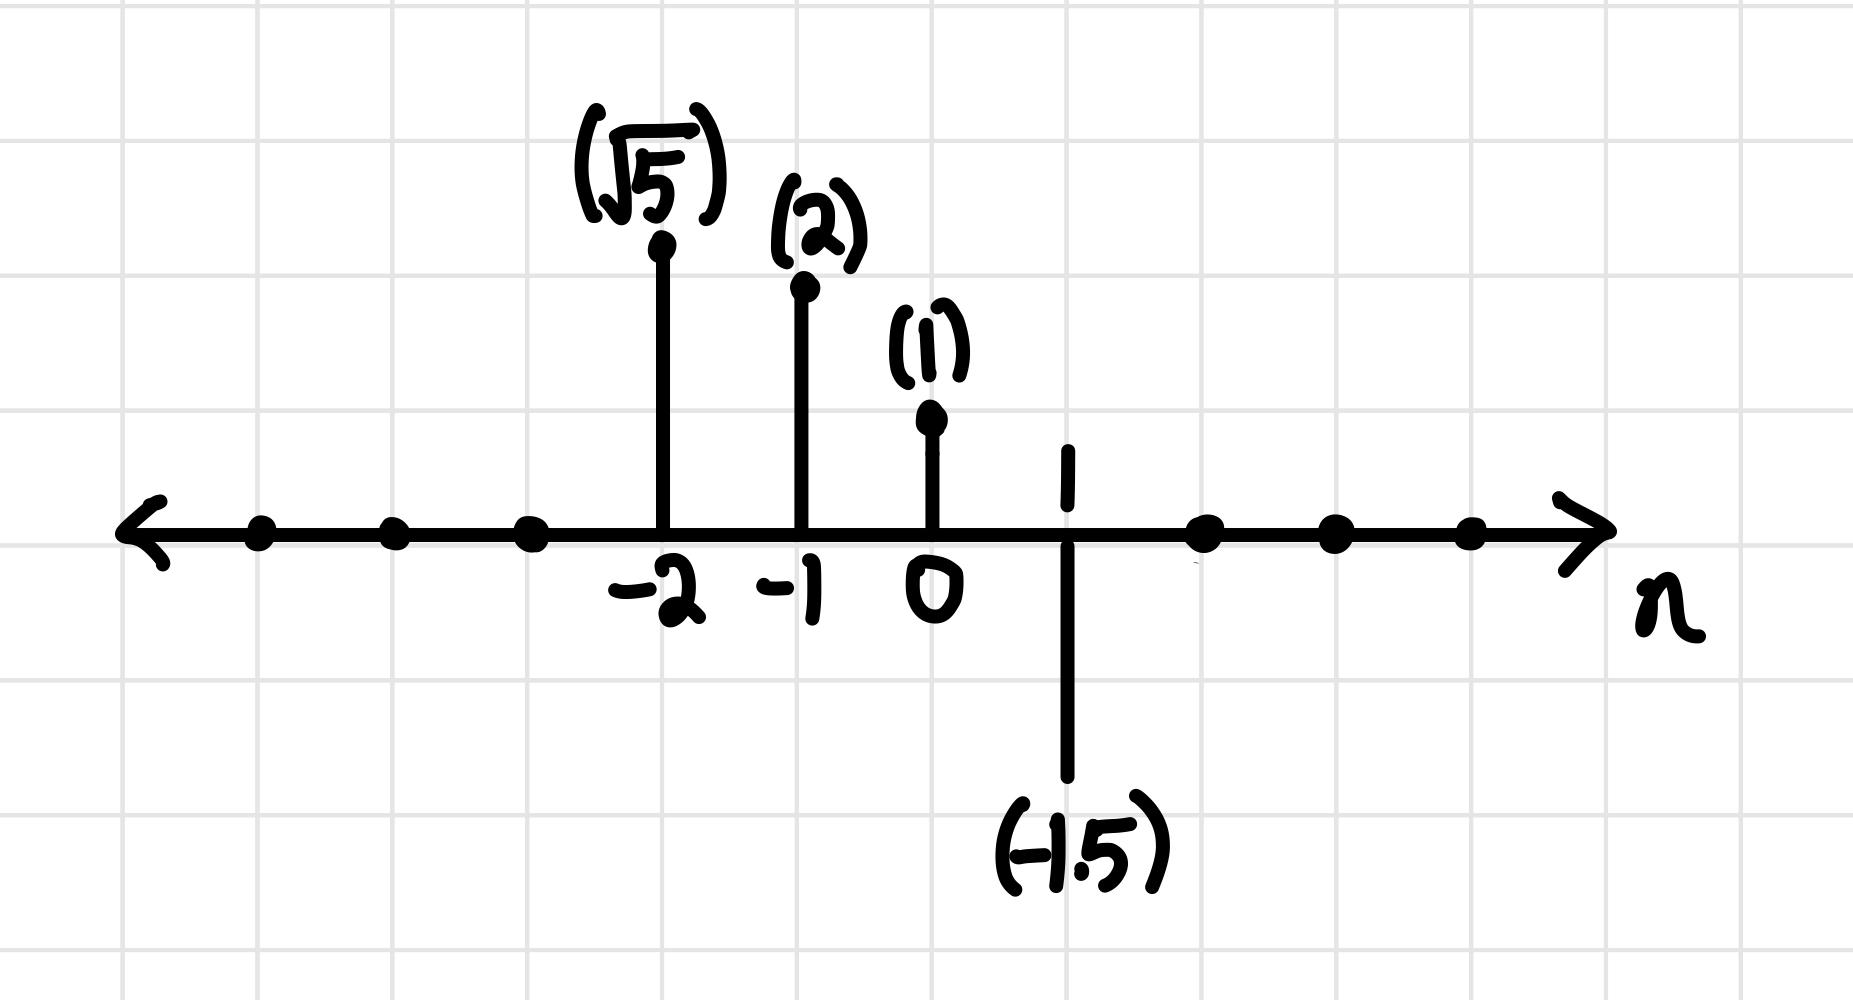
\includegraphics[ width=\textwidth/2]{lectures/img/Lec1_1.jpeg}
\end{center}

\begin{align*}
    x&: \text{function (signal in its entirety)}\\
    x(n)&: \text{value of the function $x$ evaluated at sample $n$}
\end{align*}
Thus, we have
\begin{align*}
    x(-2) &= \sqrt5 \\
    x(0.5) &= \text{undefined}
\end{align*}

\subsubsection{Example 2: CT Signal}
\begin{center}
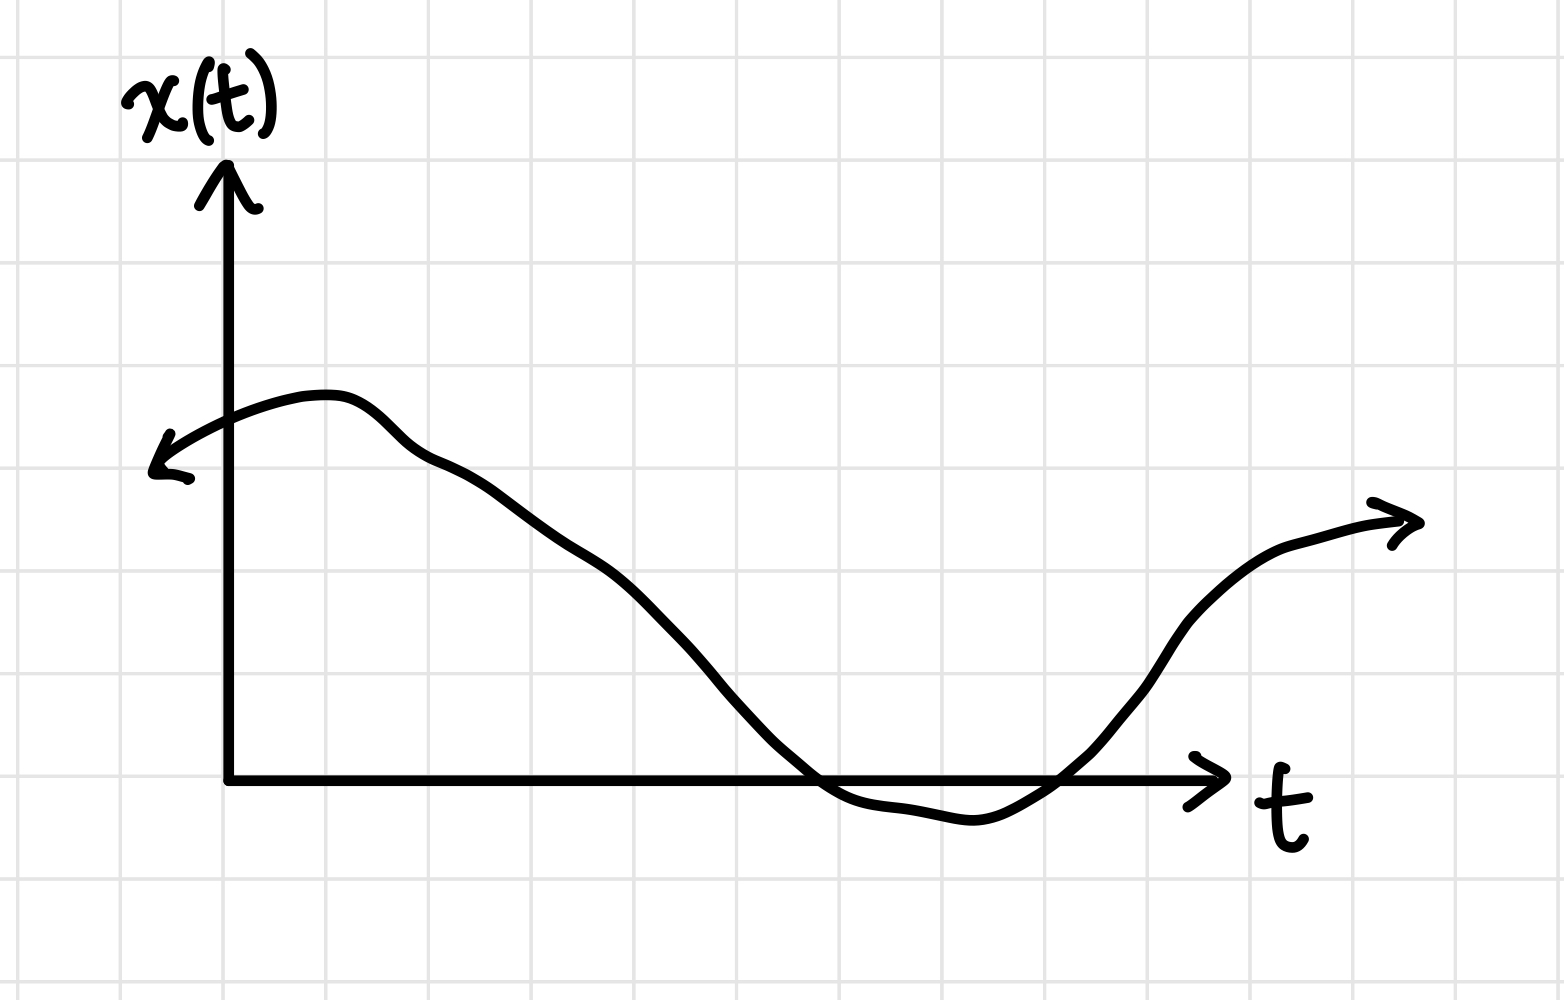
\includegraphics[ width=\textwidth/2]{lectures/img/Lec1_2.jpeg}
\end{center}

\subsubsection{Kronecker Delta (DT Impulse)}

\begin{center}
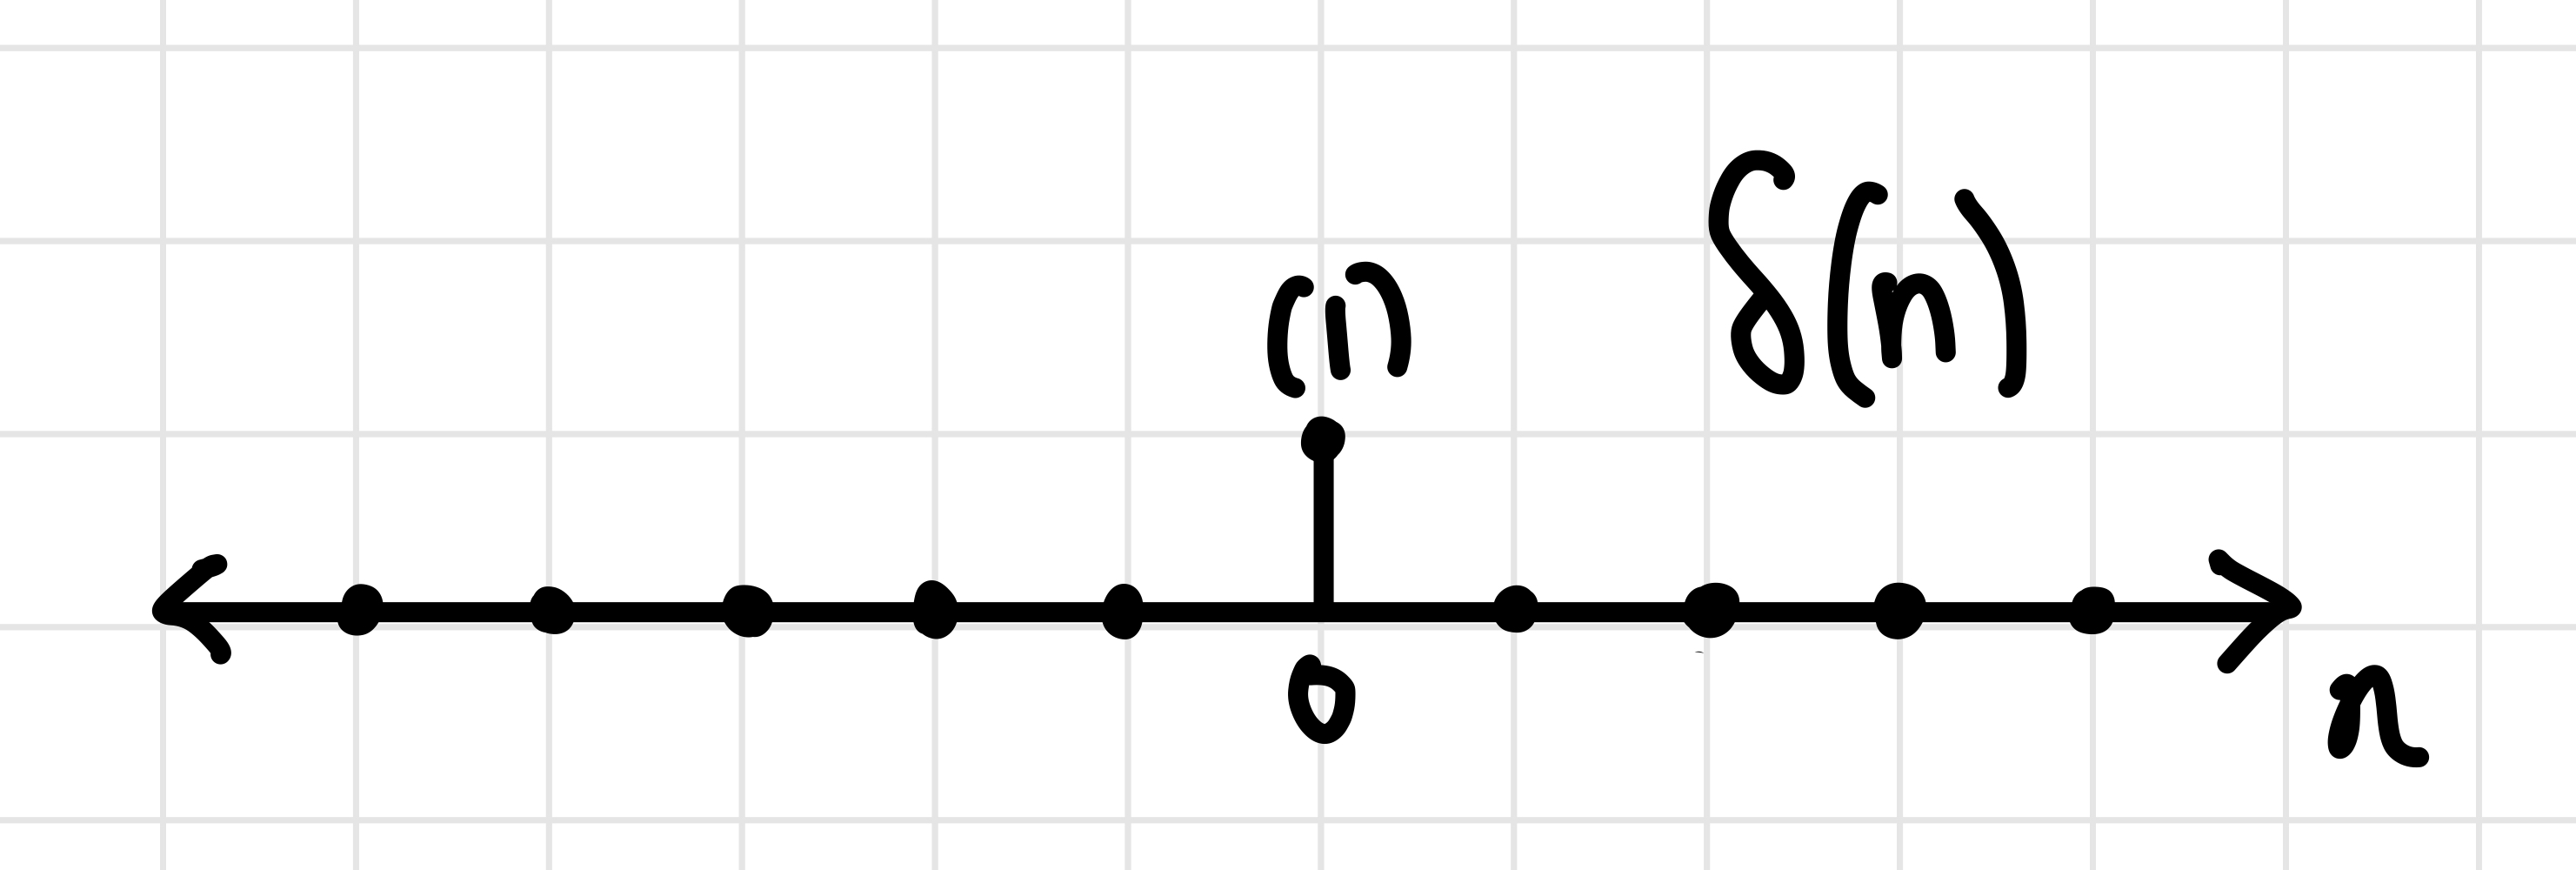
\includegraphics[ width=\textwidth/2]{lectures/img/Lec1_Delta.jpeg}
\end{center}
\[
    \delta(n) = \begin{cases}
                    1 &\text{if } n = 0\\
                    0 & \text{otherwise}
                \end{cases}
\]

Thus, we can express any DT signal in terms of a linear combination of shifted impulses.

\begin{center}
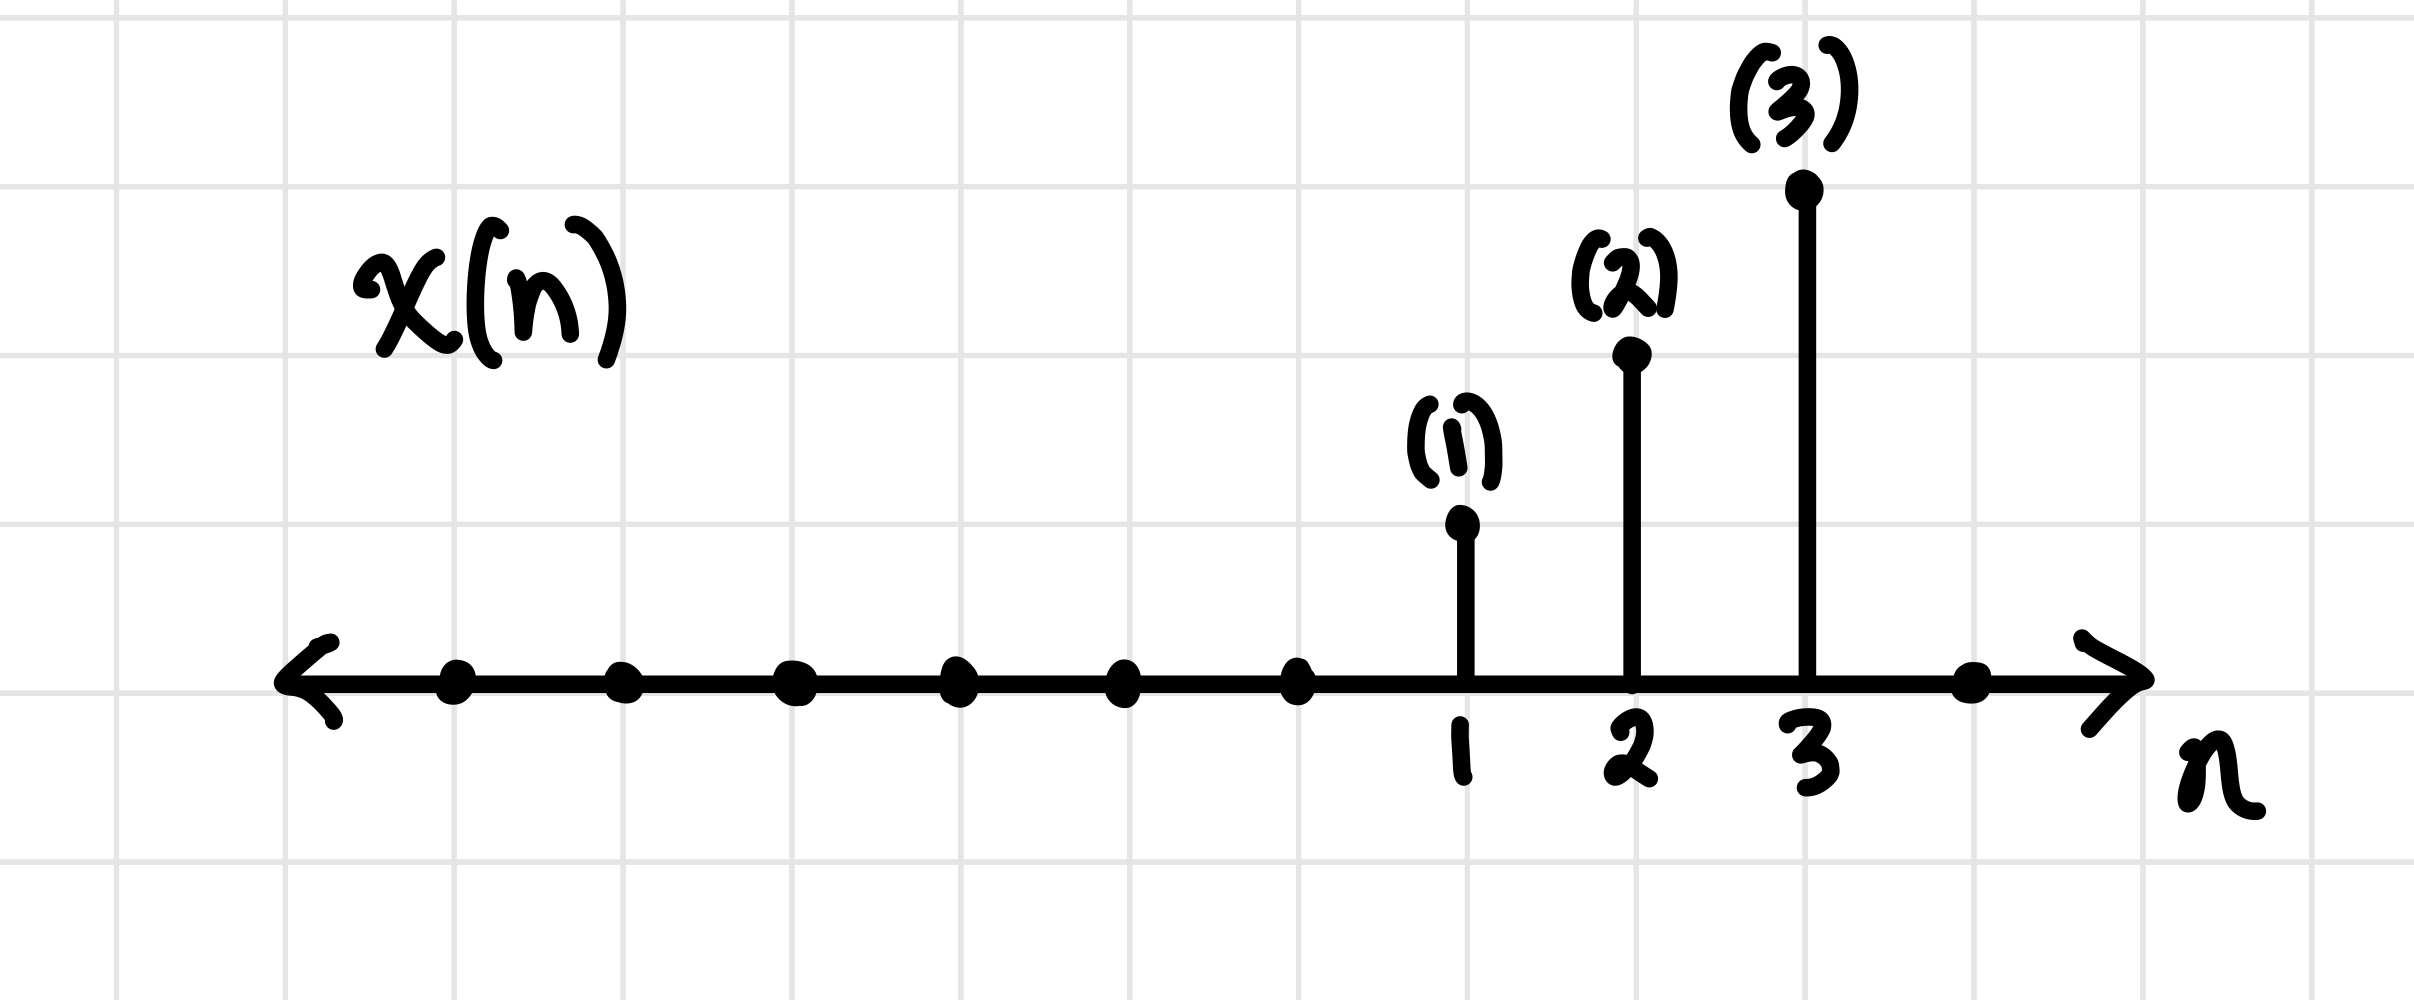
\includegraphics[ width=\textwidth/2]{lectures/img/Lec1_DeltaExample.jpeg}
\end{center}

\[x(n) = 1 \cdot \delta(n-1) + 2 \cdot \delta(n-2) + 3 \cdot \delta(n-3)\]

\subsubsection{DT Unit-Step Function}

\begin{center}
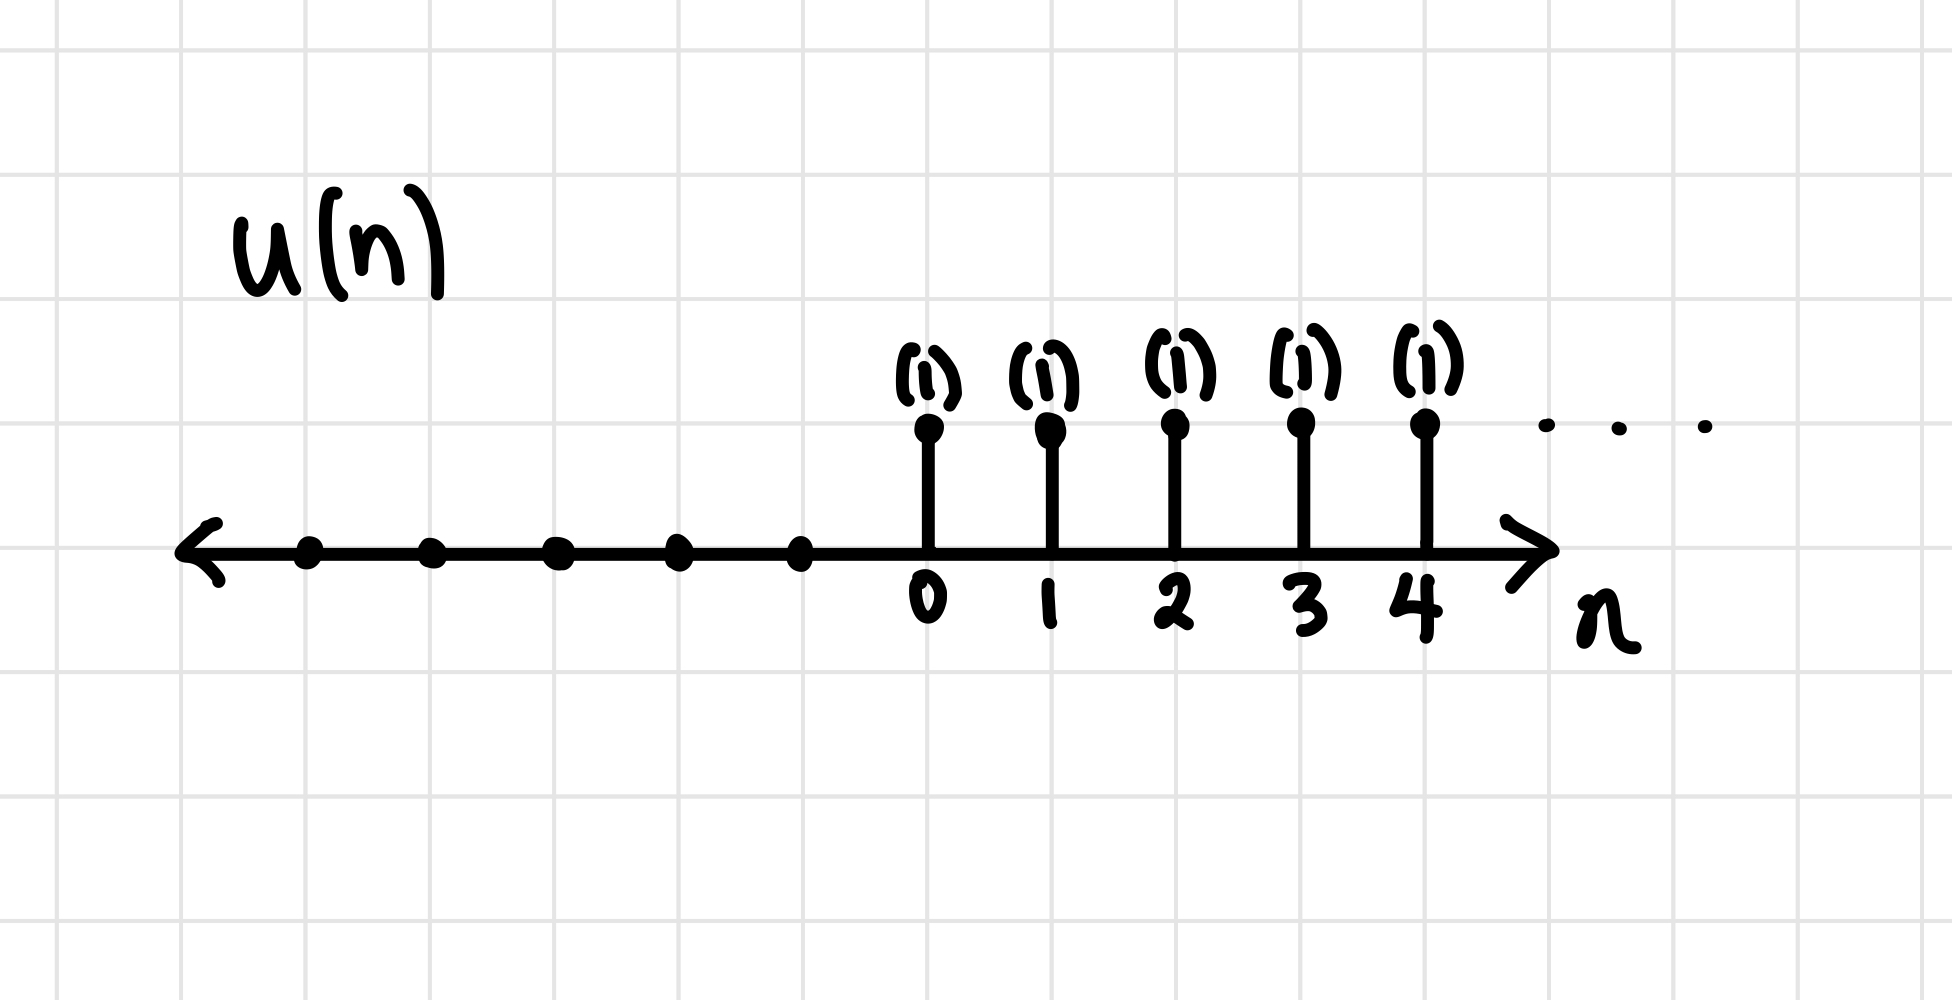
\includegraphics[ width=\textwidth/2]{lectures/img/Lec1_UnitStep.jpeg}
\end{center}

\[
    u(n)= \begin{cases}
    0 & \text{if } n < 0 \\
    1 & \text{if } n \geq 0
    \end{cases}
\]

We can actually express $u(n)$ in terms of shifted impulses ($\delta(n)$'s):
\begin{align*}
    u(n) &= \delta(n) + \delta(n-1) + \delta(n-2) + \cdots \\
    &= \sum_{k=0}^{\infty} \delta(n-k) \\
    &= \sum_{m = -\infty}^n \delta(m)
\end{align*}
Note that we do not use $i$ as an index variable since $i=\sqrt{-1}$.

Also, when we express $\delta(n)$ in terms of shifted $u(n)$, we get the following:
\[\delta(n)=u(n) - u(n-1)=\frac{u(n) - u(n-1)}{1}\]
This is a discrete-time derivative (slope).\textbf{ Impulse is the derivative of the unit step.} This will still hold in CT.

\subsection{Systems}

\textbf{Systems are also functions.
}

We can define system $F$ as a function/mapping between signal spaces $X$ and $Y$: \\
\[
\tikzmark{name}F: \tikzmark{a}X \to \tikzmark{b}Y
\] 
\begin{tikzpicture}[remember picture,overlay]
\draw[<-] 
  ([shift={(2pt,-2pt)}]pic cs:a) |- ([shift={(-10pt,-10pt)}]pic cs:a) 
  node[anchor=east] {Input Signal Space};
\draw[<-] 
  ([shift={(2pt,-2pt)}]pic cs:b) |- ([shift={(14pt,-10pt)}]pic cs:b) 
  node[anchor=west] {Output Signal Space};
\end{tikzpicture}

The systems we deal with in this class are \textbf{Single-Input, Single-Output (SISO)} systems.

Note that the inputs and outputs to $F$ are \textbf{signals}, i.e. functions. For example, $F$ may map $x_1(t) = \cos(t)$ to $y_1(t) = \sin(3t)$ where $x_1 \in X, y_1 \in Y$. Thus, we can think of the system $F$ as a mapping between sets of functions. Note that by definitions of functions, the entirety of the domain must be covered.

If $X = [\mathbb{R} \rightarrow \mathbb{R}]$ (i.e. space of real-valued CT signals) and $Y = [\mathbb{R} \rightarrow \mathbb{R}]$, then \textbf{$F$ is a Continuous-Time (CT) System}.

If $X = [\mathbb{Z} \rightarrow \mathbb{R}]$ (i.e. space of real-valued DT signals) and $Y = [\mathbb{Z} \rightarrow \mathbb{R}]$, then \textbf{$F$ is a Discrete-Time (DT) System}.

\subsubsection{Linearity}
Suppose we have a system $F: X \rightarrow Y$. We say that $F$ is linear if for all $x_1, x_2 \in X$, the following two properties hold:
\begin{align*}
    \text{Homogeneity/Scaling} & : F(\alpha x_1) = \alpha F(x_1) \\
    \text{Additivity} & : F(x_1 + x_2) = F(x_1) + F(x_2)
\end{align*}
This is also known in physics as superposition.

Next Time:
Time Invariance
 % Note that I use include over input to force new page!
    % \section{Tuesday, August 30th}
\subsection{Review: LTI (Linear Time-Invariant) Systems}

\subsubsection{Signals are functions}
    \begin{align*}
    &\text{Continuous Time: } x : \mathbb{R} \rightarrow \mathbb{R} 
    \text{ or } x : \mathbb{R} \rightarrow\mathbb{C}
    \\
    &\text{Discrete Time: } x :  \mathbb{Z} \rightarrow \mathbb{R} \text{ or } \mathbb{C}
    \end{align*}
    \[
        x \in X \ \rightarrow \ \boxed{H} \ \rightarrow \  y \in Y
    \]
    where $X$ is the input signal space and $Y$ is the output signal space.
    
    Formally, we say that $y=H(x)$. Note that systems are simply mappings from functions to functions.
    
\subsubsection{Time Invariance}
    \begin{shaded}
    If $\hat x(t)\stackrel{.} = x(t-T)$ then $\hat y(t) \stackrel.= y(t-T)$. In other words, the output must be offset at the same relative amount as the input.
    \end{shaded}
    
\subsubsection{Easy Check for LTI: ZIZO}
    To make sure that linearity is ensured, zero should map to zero. Note that this alone is not enough to prove linearity but it is necessary (e.g. $y(t)=x^2(t)$).

\subsubsection{DT-LTI General IO Derivation}
    \[
        \delta(n) \ \rightarrow \ \boxed{H} \ \rightarrow \  h(n)
    \]
    
    Time-Invariance:
    \[
        \delta(n-k) \ \rightarrow \ \boxed{H} \ \rightarrow \  h(n-k)
    \]
    
    Scaling Property:
    \[
        x(k)\delta(n-k) \ \rightarrow \ \boxed{H} \ \rightarrow \  x(k)h(n-k)
    \]
    
    Additivity:
    \[
        \underbrace{\sum_{k=-\infty}^\infty x(k)\delta(n-k)}_{x(n)} \ \rightarrow \ \boxed{H} \ \rightarrow \  \underbrace{\sum_{k=-\infty}^\infty x(k)h(n-k)}_{y(n)}
    \]
    
    The importance of LTI is that you essentially have invertibility, which allows us to uniquely describe (i.e. characterize) a signal by its impulse response. Note that LTI systems can also be seen as convolutions.

\subsubsection{Commutativity of Convolution}
\begin{shaded}
    \[
        y(n) = (x\star h)(n)=\sum_{k=-\infty}^\infty x(k)h(n-k) = \sum_{\ell = \infty}^{-\infty} x(n - \ell) h(\ell)
        = (h\star x)(n)
    \]
\end{shaded}
    
\subsubsection{Impulse Response of Cascade (Series) Interconnection}
    \[
        x(n)=\delta(n) \ \texttt{->} \ \boxed{f(n)} \ \texttt{->} \ \boxed{g(n)} \ \texttt{->} \  y(n)=(f\star g)(n)
    \]
    
which, via commutativity of convolution, has the same impulse response as the following system:
\[
        x(n)=\delta(n) \ \texttt{->} \ \boxed{g(n)} \ \texttt{->} \ \boxed{f(n)} \ \texttt{->} \  y(n)=(g\star f)(n)
    \]
    % Expect Parallel Interconnection in future lecture xor future exam


\subsection{Simple Moving Average}
\[
    x(n) \ \texttt{->} \ \boxed{h(n)} \ \texttt{->} \  y(n)=\frac1N\sum_{k=0}^{N-1} x(n-k)=\frac{x(n)+\cdots+x(n-N+1)}{N}
\]

Let us compute the impulse response of the system $H$. Letting $x(n)=\delta(n),$ we have \[y(n)=h(n)=\frac{\delta(n)+\delta(n-1)+\cdots+\delta(n-(N-1))}{N},\]
and we depict this signal below:
\begin{figure}[h]
    \centering
    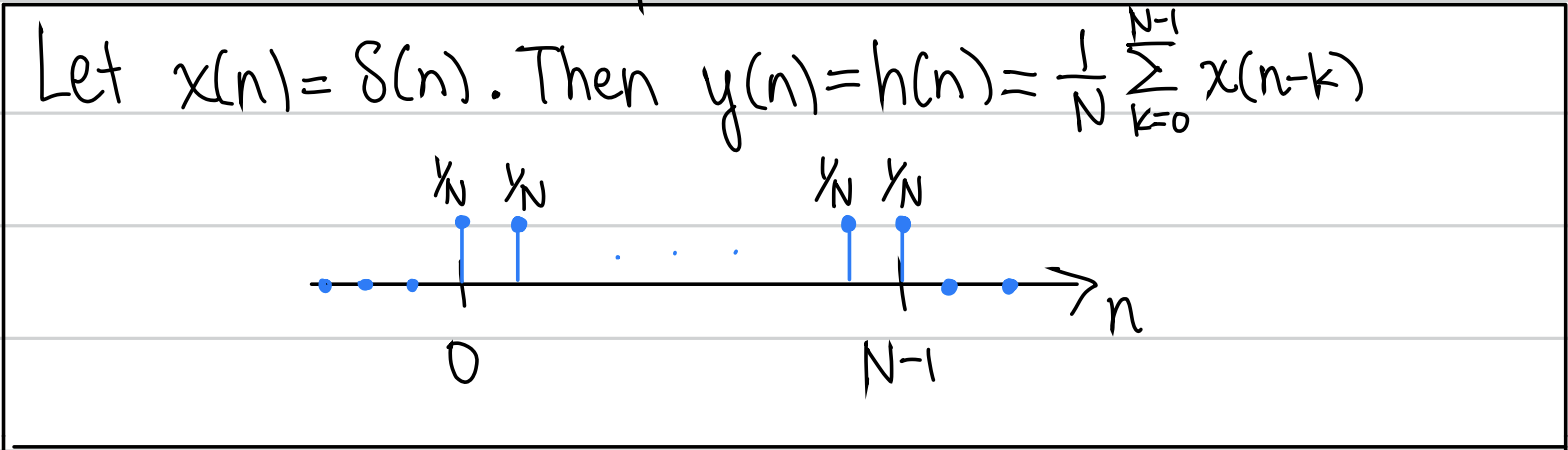
\includegraphics[scale=0.25]{lectures/img/Lec2_SimpleMovingAverage.png}
    \caption{Special thanks to Jonathan Pei for this drawing}
    \label{fig:simple_moving_average}
\end{figure}

    % \section{Thursday, June 23rd}
\subsection{Introduction}
TODO: ...

    % \section{Tuesday, September 6th}
\subsection{Euler's \& Inverse Euler's}
\subsubsection{Euler's Formula}
\[
    e^{it} = \cos(t)+i\sin(t)
\]
but the frequency (i.e. speed) can be anything:
\[
    e^{i\omega t} = \cos(\omega t)+i\sin(\omega t)
\]
where $\omega$ has units of $\frac{\text{rad}}{\text{sec}}$. Note that $f$, on the other hand, has units of $\frac{\text{cycles}}{\text{sec}}=\text{Hz}$. Also note that $2\pi$ has units of $\frac{\text{rad}}{\text{cycle}}$, which is the ratio $\omega/f$.

\begin{shaded}
Phasor: a vector that rotates around the unit circle. 

Thus, we can interpret $\omega > 0 \implies \text{CCW movement}$, and $\omega < 0 \implies \text{CW movement}$.
\end{shaded}

\begin{shaded}
Question: given $e^{i\omega t}$ and $e^{-i\omega t}$, can you get $\cos(\omega t)$?

Answer:
\[
    e^{i\omega t} + e^{-i\omega t} = 2\cos(\omega t)
    \implies
    \boxed{\cos(\omega t)=\frac{e^{i\omega t} + e^{-i\omega t}}{2}}
\]
\end{shaded}

\subsubsection{Even and Odd functions}

Cosine is an even function:
\[
    \cos(-t) = \cos(t)
\]
and Sine is an odd function:
\[
    \sin(-t) = -\sin(t)
\]

\subsubsection{Inverse Euler's}
\begin{shaded}
Question: given $e^{i\omega t}$ and $e^{-i\omega t}$, can you get $\sin(\omega t)$?

Answer:
\[
    e^{i\omega t} - e^{-i\omega t} = 2i\sin(\omega t)
    \implies
    \boxed{\sin(\omega t)=\frac{e^{i\omega t} - e^{-i\omega t}}{2i}}
\]
\end{shaded}

\subsection{Periodicity}
You have probably seen periodicity before in simple harmonic motion (without dampening) in a Physics class' dynamics unit.

Here is a nice story otherwise:
\begin{shaded}
This story of Romeo and Juliet is taken from a Cornell Professor.

Romeo proposes to Juliet and she rejects him. The rejection discourages him but later on she decides to give him a chance. But being discouraged, he rejects her, discouraging her, but the proposal now makes him interested. And so the \textbf{cycle} continues.
\end{shaded}
This is an example of \textit{cyclic behavior}.

Let us now define \textbf{CT Periodicity}.
\subsubsection{CT Periodicity}
$x:\mathbb R\mapsto \{\mathbb R \cup \mathbb C\}$ is periodic if $(\forall t\in\mathbb R),\quad x(t+T)=x(t)$ (for some) $\exists T>0 $.

We say $T$ is the fundamental period if $T$ is the smallest possible value that satisfies the periodicity relation.

Associated with the fundamental period is the fundamental frequency which is $\omega = \frac{2\pi}T \frac{\text{rad}}{\text{sec}}$ or $f=\frac1T \text{Hz}$.

If we have a constant continuous signal $x(t)=C$ for some constant $C$, then the fundamental period is undefined.

\begin{shaded}
Question: Find the period of $x(t)=\cos\left(\frac{2\pi}5 t\right)$


Answer: 
$x(t+T)=\cos\left(\frac{2\pi}5 (t+T)\right)=\cos\left(\frac{2\pi}5 t+\frac{2\pi}5 T\right)=\cos\left(\frac{2\pi}5 t\right)$

which implies $\frac{2\pi}5 T = 2\pi k\implies T=5k$ for some $k\in\{1,2,3,\ldots\}$. 

$\min k = 1 \implies T = 5 \text{ sec}$.
\end{shaded}

\newpage
\subsubsection{DT Periodicity}
If $N$ is the smallest integer such that $x(n) = x(n+N)$, we call it the fundamental period of $x$. Thus, the (fundamental) frequency is $\omega_0=\frac{2\pi}N$.

Example:
\begin{shaded}
Question: Find the (fundamental) period of $x(n)=C, \quad\forall n\in\mathbb Z$?

Answer: 
Looking at the samples (i.e. dotplot — which is just $C$ for all $n$), we can see that $N= 1$ is the fundamental period if the DT signal is constant with $\omega_0=2\pi\frac{\text{rad}}{\text{sample}}$.
\end{shaded}

Example:
\begin{shaded}
Question: Find the fundamental period and frequency of $x(n)=e^{in}, \quad\forall n\in\mathbb Z$?

Answer:
This must hold $(\forall n\in\mathbb Z),$
\[
    e^{i(n+N)} = e^{in}e^{iN} = e^{in}
\]
for some $N\in\mathbb Z$.

But $N=2\pi k\not\in\mathbb Z$.

Therefore the answer is \textbf{not} $2\pi$ as that is not an integer. Therefore the period is undefined.

We can see this graphically as we see that this jumps around the unit circle, never visiting the same point again.
\end{shaded}

Example:
\begin{shaded}
Question: Find the fundamental period and frequency of $x(n)=e^{i\frac\pi4n}, \quad\forall n\in\mathbb Z$?

Answer:
This must hold $(\forall n\in\mathbb Z),$
\[
    e^{\frac\pi4i(n+N)} = e^{\frac\pi4in}e^{\frac\pi4iN} \stackrel{\text{Want}}= e^{\frac\pi4in}
\]
for some $N\in\mathbb Z$.

which happens when $e^{\frac\pi4iN}=1\implies \frac\pi4N=2\pi k\implies k = 1\implies N = 8$.

Therefore we have (fundamental) frequency $\omega_0=\frac{2\pi}8=\frac\pi4$
\end{shaded}

\subsubsection{Necessary and Sufficient Conditions for DT Periodicity}
Now we shall examine the necessary and Sufficient Conditions for $e^{i\omega n}$ to be periodic in $n$.

\[
    e^{i\omega (n+N)} = e^{i\omega n}
\]
\[
    \cancel{e^{i\omega n}}e^{i\omega N} = \cancel{e^{i\omega n}}
\]
\[
    \boxed{e^{i\omega N} = 1}
\]

Now, noting that $\omega$ must be a rational multiple of $\pi$, we get that:
\[
    \omega N = 2\pi k \implies N=\frac{2\pi k}\omega\stackrel{^\dagger}=\frac{2\pi}{\frac l m \pi}k = \frac{2m}l k
\]
\[
    ^\dagger\omega = \frac{2\pi}N k \implies \frac l m = \frac{2k}N\implies \omega\triangleq\frac l m \pi
\]

\subsubsection{CT Periodicity}
\[
    x(t) = e^{i\omega t}
\]
appears to imply that the sky is the limit for $omega$ (i.e. $\omega\to\infty$).

We note that the oscillations become progressively faster.

Slowest frequency is $\omega = 0$ (constant signal).

\subsubsection{DT Slowest Frequency}
Slowest frequency is $\omega = 0\frac{\text{rad}}{\text{sample}}$.

\subsubsection{Fastest Frequency for Oscillating DT Signal}
For odd multiples of $\pi$,
\[
    e^{i\pi n} = \cos(\pi n) = (-1)^n
\]

\subsection{Filters}
There are 3 types:
\begin{itemize}
    \item Low-Pass Filter
    \item High-Pass Filter
    \item Band-Pass Filter
\end{itemize}

\subsection{Frequency Response of DT-LTI Systems}
There is a special relationship that exists between the Kronecker Delta.
\[
    \delta(n) \ \texttt{->} \ \boxed{H} \ \texttt{->} \  y=\underbrace{h(n)}_\text{impulse response}
\]

and we have this
\[
    x(n) = e^{i\omega n} \ \texttt{->} \ \boxed{H} \ \texttt{->} \  \underbrace{y(n)}_\text{special form}
\]

Now we can convolve:
\begin{align*}
    y(n) &= (h\ast x)(n)
    \\
    &= \sum_m h(m)e^{i\omega(n-m)}
    \\
    y(n) &= \underbrace{\sum_m h(m) e^{-i\omega m}}_{H(\omega)} e^{i\omega n}
\end{align*}

\[
    e^{i\omega n} \ \texttt{->} \ \boxed{\stackrel H h} \ \texttt{->} \  H(\omega)e^{i\omega n}
\]

This is analogous to eigenvalues: $\mathbf A\vec v=\lambda \vec v$ where $\lambda = H(\omega)\in\mathbb C$, $\vec v = e^{i\omega n}$, and where $\mathbf A=$ the system (the box).

We call $H(\omega)$ the frequency response of the LTI system, obtained by plugging the impulse response into the summation: $$H(\omega)=\sum_{m=-\infty}^\infty h(m) e^{-i\omega m}$$.

This property is known as the Eigenfunction Property of Complex Exponentials with respect to a DT-LTI System.

\subsubsection{Modulation}
\[
  x(n) \ \texttt{->} \ \stackrel{\stackrel{e^{i\omega_1 n}}{\stackrel{|}{\texttt{v}}}}{\boxed{X}} \ \texttt{->} \ y(n) = e^{i\omega_1 n}x(n) = e^{i(\omega_0+\omega_1) n}
\]

\subsubsection{DT LTI Valid Examples}
\[
    \alpha_0e^{i\omega_0 n}+\alpha_1e^{i\omega_1 n} \ \texttt{->} \ \stackrel{\text{LTI}}{\boxed{H}} \ \texttt{->} \  \alpha_0H(\omega_0)e^{i\omega_0 n}
    +
    \alpha_1H(\omega_1)e^{i\omega_1 n}
\]
If for example, we saw another $\alpha_2H(\omega_2)e^{i\omega_2 n}$ term then we would know our system is \textbf{not} LTI.

\subsubsection{Frequency Response of 2-pt Moving Average filter}
We want to find the frequency response for the 2-pt moving average filter:
\[
    x(n) \ \texttt{->} \ \boxed{H} \ \texttt{->} \ y(n) = \frac{x(n)+x(n-1)}2
\]
Note that if $x(n)=(-1)^n=e^{i\pi n}\implies y(n)=0\quad\forall n$.

However if $x(n)=1=e^{i0n}\implies y(n)=1\quad\forall n$.

Sanity check values:
\[
    H(\omega=0) = 1
\]
\[
    H(\omega=\pi) = 0
\]

Finding the frequency repsonse:
\begin{shaded}
Let $x(n)=\delta(n) \implies h(n)=\frac{\delta(n)+\delta(n-1)}2$

then we note the dotplot is $\frac12$ at $n=0$ and $n=1$ and $0$ everywhere else.
\end{shaded}
Now, we can compute the expression as follows:
\begin{align*}
    H(\omega) &= \sum_m h(m) e^{-i\omega m}
    \\
    &= h(0) + h(1) e^{-i\omega}
    \\
    H(\omega) &= \frac{1+e^{-i\omega}}2
\end{align*}


    % \section{Thursday, September 8th}
\subsection{Overview}
DT Frequency Response:
\begin{itemize}
    \item 2 point Moving Average Filler
    \item Recursive Filter
\end{itemize}
\subsection{DT Frequency Response}
\subsection{2-Point Moving Average Filter}
\subsection{Computing \texorpdfstring{$H(\omega)$}{H(w)}}
\subsubsection{Example: Using 2-pt moving average}
\subsection{Plotting Frequency Response}
\subsubsection{Example: using 2-pt moving average}
\subsection{\texorpdfstring{$2\pi$}{2pi}-Periodicity of DT-LTI Frequency Response}
\subsection{DAG (Delay-Adder-Gain) Block Diagram Implementation}
\subsection{The Big Picture}
\subsection{LTI System w/o LCCDE Representation}
\subsection{Finite-Duration Impulse Response}
\subsubsection{FIR (Finite Impulse Response) Filter}
\subsection{Infinite-Duration Impulse Response}
\subsubsection{IIR (Infinite Impulse Response) Filter}
\subsection{Frequency Response for Recursive Filler}
\includepdf[pages=14-]{lectures/wk2/09_08_2022_EE120_Notes.pdf}

    % \section{Thursday, September 15th}
\subsection{IIR Filter Frequency Response}
Given a First-Order IIR (Infinite Impulse Response, vs Finite Impulse Response)
\begin{align*}
    y(n)
    &=
    \alpha y(n=1)+x(n)
    \\
    y(-1)
    &=
    0
    \\
    |\alpha|
    &<
    1
\end{align*}

\begin{align*}
    x(n)
    &=
    e^{i\omega n} \to y(n)=H(\omega)e^{i\omega n}
    \\
    y(n-1)
    &=
    H(\omega)e^{i\omega (n-1)} = H(\omega)e^{-i\omega}e^{i\omega n}
\end{align*}

\begin{align*}
    H(\omega)\cancel{e^{i\omega n}} 
    &= \alpha H(\omega)e^{-i\omega}\cancel{e^{i\omega n}}+\cancel{e^{i\omega n}}
    \\
    (1-\alpha e^{i\omega})H(\omega) 
    &= 1
    \\
    H(\omega) 
    = \frac1{1-\alpha e^{i\omega}} 
    = |H(\omega)|e^{i\angle H(\omega)}
\end{align*}

\begin{align*}
    H(\omega) 
    &= \frac1{1-\alpha e^{i\omega}}
    \\
    |H(\omega)| 
    &= \left|\frac1{1-\alpha e^{i\omega}}\right|
    &&\text{[By property \eqref{eq:1}]}
    \\
    &= \frac1{|1-\alpha e^{i\omega}|}
    \\
    &= \frac1{|1-\alpha\cos(\omega)+i\alpha\sin(\omega)|}
    \\
    &= \frac1{\sqrt{(1-\alpha\cos(\omega))^2+\alpha^2\sin^2(\omega)}}
\end{align*}

\subsubsection{Properties}
\begin{equation}\label{eq:1}
    \left|\frac{z_1}{z_2}\right| = \frac{|z_1|}{|z_2|}
\end{equation}
\[
    \angle \frac{z_1}{z_2} = \angle z_1 - \angle z_2
\]

\subsubsection{Plot}
\begin{equation}\label{eq:2}
    H(\omega) 
    = \frac{e^{i\omega}}{e^{i\omega}-\alpha}
    = \frac1{1-\alpha e^{i\omega}}
\end{equation}

At $\omega = 0$, we have the max response.\\
At $\omega = \pm\pi$, we have the min response.\\
Therefore, this is a Low-Pass Filter; see the plot here:
\href{https://www.desmos.com/calculator/oa25atozja}{https://www.desmos.com/calculator/oa25atozja}.

\begin{align*}
    H(\omega) 
    &= \sum_{n=-\infty}^\infty h(n) e^{-i\omega n}
    = \sum_{n=0}^\infty \alpha^n e^{-i\omega n}
    \\
    &= \sum_n |h(n) e^{-i\omega n}| < \infty
\end{align*}

\begin{shaded}
Q: How to make this (eq \eqref{eq:2}) low-pass filter into a high-pass filter?

A: Set $\alpha$ to be in the region $(-1, 0)$, with $\alpha=-1$ being the sharpest high-pass filter possible. This makes sense as we have a min when $\omega=0$ at $\frac1{1-\alpha}$ and maxima at $\pm\pi$.
\end{shaded}

\begin{shaded}
Q: How to make this (eq \eqref{eq:2}) peak at $\omega=\frac\pi4$?

A: We can set $\alpha=\lambda e^{i\frac\pi4}$ where $0\le|\lambda|\le1$ determines the aggressiveness of the filter.
\end{shaded}

\subsection{System Properties}
\begin{align*}
    \angle H(\omega) 
    &= \angle \frac{e^{i\omega} - 0}{e^{i\omega}-\alpha}
    \\
    &= \angle{(e^{i\omega} - 0)} - \angle{(e^{i\omega}-\alpha)}
    &&\text{[The phase is the difference in phases of the 2 vectors]}
    \\
    \omega=0
    &\implies\angle H(\omega) = 0
    &&\text{[Both are at 1, }0\le\alpha\le1]
\end{align*}
Plot: \href{https://www.desmos.com/calculator/rvkvjzwhws}{https://www.desmos.com/calculator/rvkvjzwhws}

Think of a system which delays the input by $N,\  (\forall N\in\mathbb Z^+)$, samples (or the system which advances the input by $N,\  (\forall N\in\mathbb Z^-)$, samples):

\newpage
\subsubsection{Causality}
\textbf{Does not peek ahead in time}

Discrete Causality (note that continuous is similar, without the constraint on $N$):\\
We say $H$ is causal if for every integer N,
if it is the case that two signals $x_1, x_2\in X$ (where $X$ is the input space) are equal up to (and including) $n=N:$ 
\\
$x_1(n)=x_2(n)\quad(\forall n\le N)$ then $y_1(n)= y_2(n) \quad(\forall n\le N)$.

Example:
\begin{shaded}
Given a linear system $H$ with input $x(n)=u(n)$ and output $y(n)=\begin{cases} 
1 & n = -1\\
2 & n = 0\\
3 & n = 1\\
0 & \text{e/w}\end{cases}$.
\end{shaded}
By the ZIZO property of Linearity, we realize that the zero signal should match up to and including $x_2(n)=u(n), (\forall n\le-1),$ with Zero-In, Zero-out: so input is $x_2(n)=0, (\forall n\in\mathbb Z)$. \textbf{However}, we expect $y(-1)=0$ since $y_2(-1)=0$ but $y(-1)=-1$ so we have a contradiction.

\begin{shaded}
What if $H$ is now TI but not Linear?
\end{shaded}
Let $x_2(n)=x_1(n-1)=u(n-1)$

But then $y(-1)=1\ne y_2(-1)=0$ even though they match up to and including $-1$. So this is not causal.

\subsubsection{BIBO Stability}
Bounded-Input, Bounded-Output Stability

We say a signal $x$ is bounded if $\exists 0 < B_x < \infty$ s.t. $|x(n)|<B_x, \quad(\forall n\in\mathbb Z)$.

Graphically this can be seen as if all lollipops are bounded between (and including) $-B_x$ and $B_x$.


BIBO Stability is exactly what it says:

Given a discrete system $H$ (with no information on whether $H$ is Linear or Time Invariant),\\ 
we say that $H$ is BIBO Stable if every bounded input produces a bounded output.

Example: 3-point moving averager:
\[
    y(n) = \frac{x(n)+x(n-1)+x(n-2)}3
\]
We know $y$ is causal since it is only dependent on past value (it does not peek into the future). Specifically we can say that $h(n)=0,\quad(\forall n < 0)$.

\[
    y(n)
    = \sum_{k=-\infty}^\infty h(k)x(n-k)
    =y(n)=\underbrace{\cdots +h(-1) x(n+1)}_{\text{want to be identically zero}}+h(0) x(n)+h(1) x(n-1)+\cdots
\]
Note that this actually goes \textbf{both ways}. Mathematically that means the system is stable \textbf{if and only if} the response is 0 for all negative time.

\begin{align*}
    |y(n)|
    &= \left|\frac{x(n)+x(n-1)+x(n-2)}3\right|
    \\
    &= \frac13\left|x(n)+x(n-1)+x(n-2)\right|
    \\
    &\le \frac13\left(|x(n)|+|x(n-1)|+|x(n-2)|\right)
    \\
    &\le \frac{B_x+B_x+B_x}3=B_x-B_y
\end{align*}

All BIBO filters are stable by induction on the triangle inequality (given that all lollipops are finite and not infinite).

\subsubsection{BIBO DT-LTI Systems}
We say $H$ is BIBO-stable iff $$\sum_{n=-\infty}^\infty |h(n)| <\infty$$

Proof:
\begin{shaded}
\[
y(n)=\sum_{k=-\infty}^{\infty} h(k) x(n-k)
\]

Let $|x(n)| \leq B_x \forall n \in \mathbb{Z}$. Then we have that
\begin{align*}
|y(n)| &=\left|\sum_{k=-\infty}^{\infty} h(k) x(n-k)\right| \\
& \leq \sum_{k=-\infty}^{\infty}|h(k) x(n-k)| \\
& \leq \sum_{k=-\infty}^{k \infty}|h(k)| B_x \\
& \leq B_x \sum_{k=-\infty}^{\infty}|h(k)|<\infty \\
&=B_y
\end{align*}
for some $B_y<\infty$.
\end{shaded}

    % \section{Tuesday, September 20th}
\subsection{BIBO Stability (continued)}
We say $H$ is BIBO-stable iff $$\sum_{n=-\infty}^\infty |h(n)| <\infty$$

\subsubsection{Sufficiency}
Proof:
\begin{shaded}
\[
y(n)=\sum_{k=-\infty}^{\infty} h(k) x(n-k)
\]

Let $|x(n)| \leq B_x \forall n \in \mathbb{Z}$. Then we have that
\begin{align*}
|y(n)| &=\left|\sum_{k=-\infty}^{\infty} h(k) x(n-k)\right| \\
& \leq \sum_{k=-\infty}^{\infty}|h(k) x(n-k)| \\
& \leq \sum_{k=-\infty}^{k \infty}|h(k)| B_x \\
& \leq B_x \sum_{k=-\infty}^{\infty}|h(k)|<\infty \\
&=B_y
\end{align*}
for some $B_y<\infty$.
\end{shaded}
Definition Of BIBO Stability: Every bounded input produces a bonded output.

\subsubsection{Necessity}
The other direction of the proof.

We can start with the contrapositive (Recall that the contrapositive of $A\implies B$ is $\lnot B\implies\lnot A$).

We say that $h\in\ell^1$ if $\sum_n |h(n)|<\infty$ if h is absolutely summable, where $\ell^1$ is the space of all abs summable functions.

\begin{shaded}
Continuous Counterpart (will not go over today):

We say that $h\in\mathcal L^1$ if $\int_n |h(n)|\mathrm n<\infty$ if h is absolutely integrable, where $\mathcal L^1$ is the space of all abs integrable functions.
\end{shaded}

Let us defined the parts of the proof:
\begin{itemize}
    \item $\lnot B: h$ is not abs summable $h\not\in\ell^1$.
    \item $\lnot A: H$ is not BIBO Stable, per the previous definition.
    \item $\lnot $ BIBO Stable: $\exists$ a bounded input that produces an unbounded output.
    \begin{itemize}
        \item Various ways to do this, such as finding an input relating to input response s.t. the output at a single point blows up.
    \end{itemize}
\end{itemize}

Now we are ready to continue our proof for real-valued LTI systems:\\
We begin by choosing an input
\[
    x(n) = \sgn(h(-n)), \text{ where } \sgn(\alpha) = \begin{cases} 1\quad\alpha>0 \\ 0\quad\alpha=0 \\ -1\quad\alpha<0 \end{cases}
\]

\begin{shaded}
To understand the $\sgn$ fn., look at $v(n) = (-2)^n u(n)$

Then $\hat v(n) = \sgn(v(-n))$ which is all 0 for negative n, and then alternates between 1 and -1 for all non-negative integers. Note that we will be 0 for all negative inputs.

After time-reversing this, we will note that the mapping ($n\in\mathfrak E\mapsto 1, n\in\mathfrak O\mapsto -1$) still holds, where $\mathfrak E$ is the set of even integers and $\mathfrak O$ is the set of odd integers. Note that we will now be 0 for all positive inputs.

We know that $\hat v(n)$ is bounded as it can only ever have 3 values. To be precise: $|x(n)|\le1\quad(\forall n)$.
\end{shaded}

Using this, we can find the particular timestep at which the signal blows up:
\begin{align*}
    x(k)\triangleq\sgn(h(-k))
    &\implies
    |x(k)|\le1\ (\forall k)
    \\
    \implies
    x(k)
    &= 
    \begin{cases}\frac{h(-k)}{|h(-k)|} & \text{if } h(-k)\ne0\\ 0 & \text{e/w}\end{cases}
    &&\text{[Can be shown via L'hopitals]}
\end{align*}
\begin{align*}
    y(n) 
    &= 
    \sum_k x(k) h(n-k)
    &&\text{[Convolution Sum]}
    \\
    y(0)
    &= 
    \sum_k x(k) h(-k)
    \\
    &= 
    \sum_k \frac{h(-k)}{|h(-k)|} h(-k)
    \\
    &= 
    \sum_k \frac{|h(-k)|^2}{|h(-k)|}
    \\
    &= 
    \sum_k |h(-k)|
    \\
    &= 
    \sum_\ell |h(\ell)| \to \infty
    &&[\ell\triangleq-k]
\end{align*}
Therefore we have shown that $h\not\in\ell^1\implies\exists x, \text{ s.t. } |x(n)|\le B_x$ but the the corresponding output is not bounded. Contradiction.

Example:
\[
    y(n)=\alpha y(n-1)+x(n),\quad h(n)=\alpha^n u(n)
\]
System is BIBO stable iff $|\alpha|<1$.

Example:
\[
    h(n)=u(n)\quad h\not\in\ell^1
\]
If we convolve $h(n)$ with $x(n)$ to get $y(n)$, then we get $y(n)=\sum_{k=-\infty}^n x(k)$ which is a cumulative sum.

Let $x(n)=1\quad\forall n$, then the output at say $n=0$, but this could be any point wlog, is infinite. This is as you are taking the cumulative sum of an infinite sum of constants.

For another example of this ``blowing up'' behavior $x(n)=u(-n)=\sgn(u(-n))$ which perfectly overlaps when time-reserved giving $y(0)=\infty$. Since they both have 1 for all non-negative integer inputs.

\subsection{BIBO Stability (continued)}
A system is BIBO Stable if $|\lambda|<1$. If this condition is not satisfied tehn we do not have a frequency response. Note that in the special case of $\lambda=1$, we \textit{may} still have a frequency response exist.

If $h\in\ell^1$, (aka if the system is BIBO-stable/absolutely summable), which means the frequency response $|H(\omega)|<\infty\ \forall\omega$ and that $H(\omega)$ is continuous in $\omega$. 

\begin{align*}
    |H(\omega)| 
    &= |\sum_n h(n) e^{-i\omega n}|
    \\
    &\le \sum_n |h(n) e^{-i\omega n}|
    &&\text{[Triangle Inequality]}
    \\
    &= \sum_n |h(n)| \underbrace{|e^{-i\omega n}|}_1
    \\ 
    &= 
    \sum_n |h(n)| 
    <
    \infty
\end{align*}
    
    
Some LTI Systems have $h\not\in\ell^1$ but $h\in\ell^2$.

Example from Calculus: Harmonic Series $=\sum \frac1n\not<\infty$ but $\sum \frac1{n^2}<\infty$.

The ideal LPF $=\begin{cases}
G_0 \quad \forall \omega\in(-\omega_c, \omega_c)
\\
0 \quad \text{e/w}.
\end{cases}$
which is a discontinuous boxcar, \\
and $|\omega_c|<\pi$ as we are Low-Pass.

Another example is $h(n)=G_0\frac{\sin(\omega_c n)}{n\pi}$.

For $\ell^n,$ where $n > 2$, all bets are off. At the end of the semester we can use Laplace or Z-Transforms but we cannot say anything about their frequency responses as they may not even exist.

Ideally we have $\ell^1$, but we can deal with $\ell^2$; however if we have $\ell^n, n>2$ then all bets are off.

\subsection{LCCDEs \& Freq Resp.}
Not all are LCCDE, but those that are have nice Freq Resp.

\begin{equation*}
    a_0 y(n) + a_1 y(n - 1) + \cdots +  a_N y(n - N) 
    = b_0 x(n) + b_1 x(n-1) + \cdots + b_M (xn-M)
\end{equation*}
\begin{equation}\label{eq:3}
    \sum_{k=0}^N a_k y(n-k) = \sum_{m=0}^M b_m x(n-m)
\end{equation}

Recall that for $y(n) = \alpha y(n-1) + x(n)$ or:\\
$\underbrace{1}_{a_0}y(n) - \underbrace{1}_{a_1}\alpha y(n-1) = \underbrace{1}_{b_0}x(n),\ M=0,\ N=1$ where $\max(N, M) = $ order of the system.

    
\begin{align*}
    \text{Let } x(n) 
    &=
    e^{i\omega n},
    \\
    y(n) 
    &= 
    H(\omega)e^{i\omega n}
    \\
    y(n-k) 
    &= 
    H(\omega)e^{i\omega (n-k)}
    \\
    y(n-k) 
    &= 
    H(\omega)e^{-i\omega k} e^{i\omega n}
    \\
    x(n-m) 
    &= 
    e^{i\omega(n-m)]} = e^{-i\omega m}e^{i\omega n}
\end{align*}

Plugging into \eqref{eq:3},
\begin{align*}
    \sum_{k=0}^N a_k H(\omega)e^{-i\omega k}\cancel{e^{i\omega n}}
    &=
    \sum_{m=0}^M b_m e^{-i\omega m}\cancel{e^{i\omega n}}
    \\
    \left(\sum_{k=0}^N a_k e^{-i\omega k}\right)H(\omega)
    &=
    \sum_{m=0}^M b_m e^{-i\omega m}
    \\
    &\implies
    H(\omega)
    = 
    \frac{\sum_{m=0}^M b_m e^{-i\omega m}}{\sum_{k=0}^N a_k e^{-i\omega k}}
    &&\text{[which is rational in $e^{i\omega}$]}
\end{align*}

Let $H(z)=\frac{B(z)}{A(z)},\quad B(z)=M^{\text{th}}$ order polynomial. 
$A(z)=N^{\text{th}}$ order polynomial.\\
$H(z)$ is rational in $z$.

First order ($\max(M,N)=\max(0,1)=1$) IIR Filter: $H(\omega)=\frac b{a_0+a_1= e^{-i\omega}} = \frac1{1-\alpha e^{-i\omega}}$

\subsection{LCCDEs \& State-Space Resp.}
\begin{align*}
    q(n+1) 
    &= Aq(n)+Bx(n)
    &&\text{[State-Evolution Eqn.]}
    \\
    y(n) 
    &= Cq(n) + Dx(n)
    &&\text{[Output Eqn.]}
    \\
    q(n)
    &=\begin{bmatrix}
        q_1(n)
        \\
        \vdots
        \\
        q_N(n)
    \end{bmatrix}
\end{align*}

$x, y\in\mathbb R^1$, $A_{N\times N}$ is the state-transition matrix.\\
$B_{N\times 1}$ is a column vector, $C_{1\times N}$ is a row vector, $D_{1\times1}$ is a scalar.

Giving the current charge of the capacitor (a memory element) of a circuit, you do not care how it got there.

Example: $y(n)+a_1 y(n-1) + a_2 y(n-2) = x(n)$.

Note that this LCCDE example is particularly shifted as it doesnt have any delayed (shifted) term in $x$. Specifically, we can use this trick:

Pick $q_1(n)=y(n-1), q_2(n)=y(n-2)$ such that $q_1(n)=q_2(n+1)$, \\
where we picked all $y(n-k)\ \forall k\ne0$.

Note that the order of this system is $\max(0, 2) = 2$ which makes $\dim(A) = 2\times 2$.

\begin{align*}
    \begin{bmatrix}
        q_1(n+1)
        \\
        q_2(n+1)
    \end{bmatrix}
    &=
    \underbrace{
    \begin{bmatrix}
         & 
        \\
        1 & 0 
    \end{bmatrix}
    }_\text{A}
    \begin{bmatrix}
        q_1(n)
        \\
        q_2(n)
    \end{bmatrix}
    +
    \underbrace{
    \begin{bmatrix}
        \ 
        \\
        0
    \end{bmatrix}
    }_\text{B}
    x(n)
    \\
    \implies
    q_1(n+1)
    = y(n)
    &= 
    -a_1\underbrace{y(n-1)}_{q_1(n)} -a_2\underbrace{y(n-2)}_{q_2(n)} + x(n)
    \\
    &= -a_1 q_1(n) -a_2 q_2(n) + x(n)
    \\
    y(n)
    &=
    \underbrace{
    \begin{bmatrix}
        -a_1 & -a_2
    \end{bmatrix}}
    _C
    \begin{bmatrix}
        q_1(n) 
        \\ 
        q_2(n)
    \end{bmatrix}
    + 
    \underbrace{1}_D x(n)
\end{align*}
    % \section{Thursday, September 22th}
\subsection{LCCDEs \& State-Space Resp. (continued)}
Draw a Delay-Adder-Gain (DAG) block diagram with minimum number of \textit{delay} blocks:
\begin{figure}[h]
    \centering
    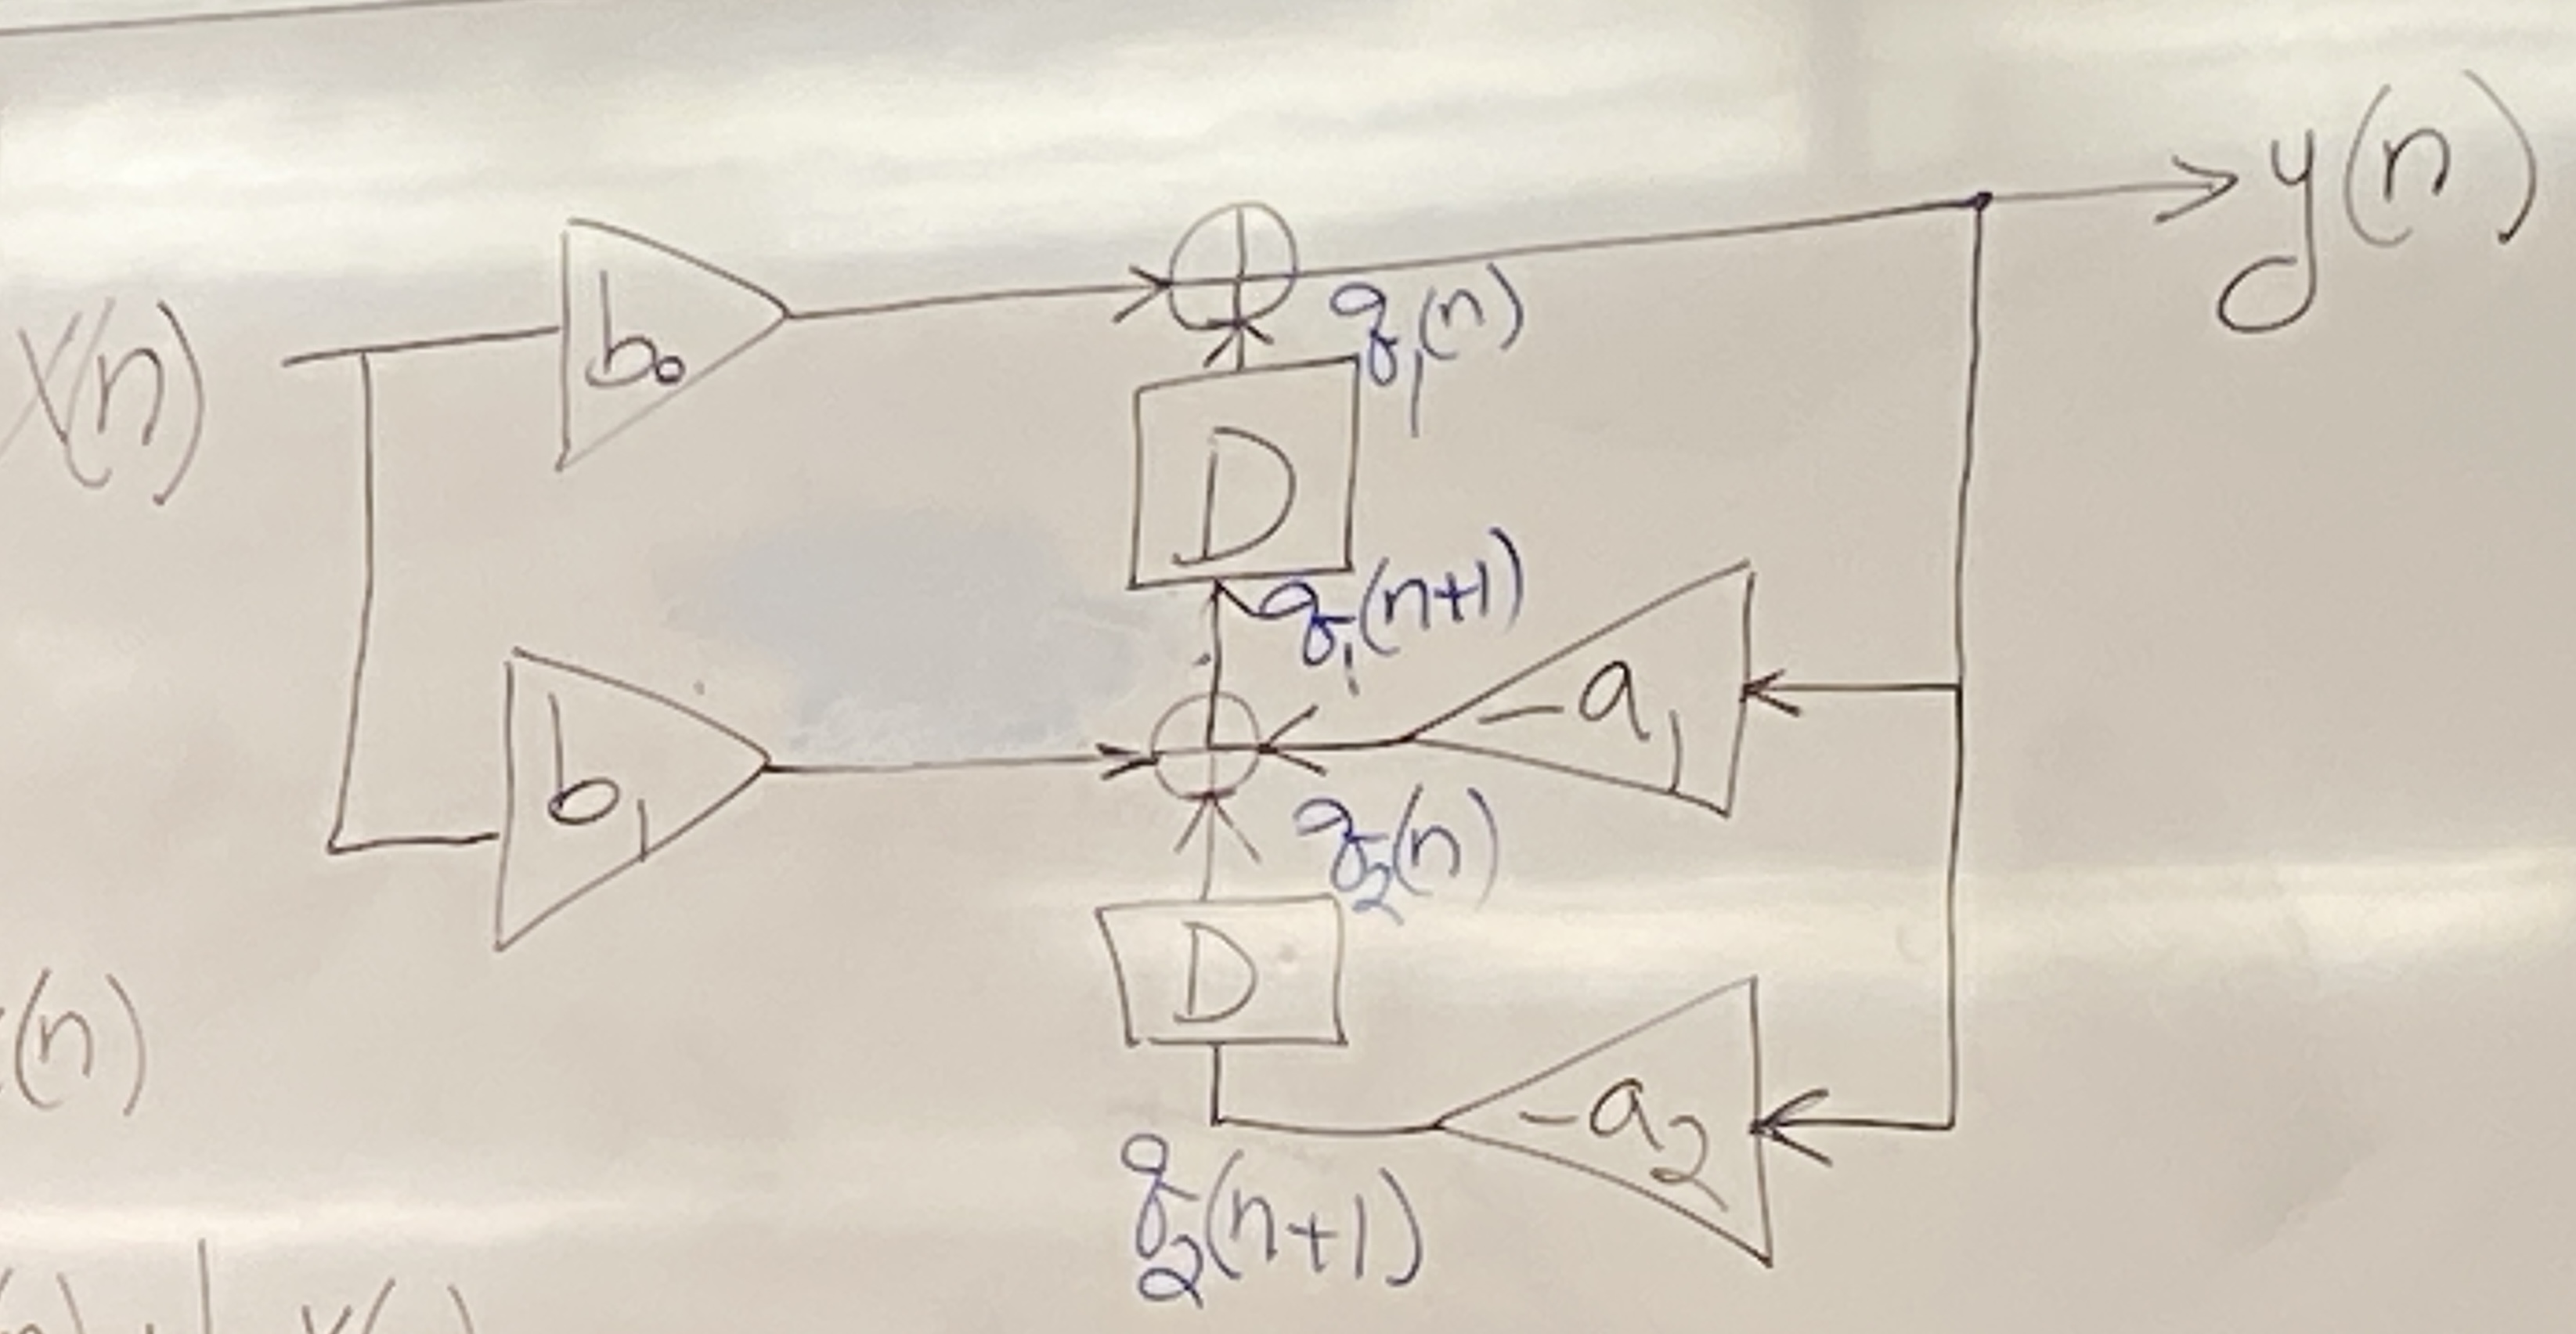
\includegraphics[scale=0.1]{lectures/img/Lec8_DAG.jpg}
    \label{fig:lec8_dag}
\end{figure}

\begin{align*}
    q(n+1) &= A q(n) + B x(n)
    \\
    y(n) &= C q(n) + D x(n)
    \\
    q(n) &= \begin{bmatrix}
        q_1(n) \\ q_2(n)
    \end{bmatrix}
\end{align*}

\begin{align*}
    y(n)
    &= q_1(n) + b_0 x(n)
    \\
    &= \underbrace{\begin{bmatrix}
        1 & 0
    \end{bmatrix}}_C \begin{bmatrix}
        q_1(n)\\
        q_2(n)
    \end{bmatrix}
    + \underbrace{b_0}_D x(n)
    \\
    q_1(n+1)
    &= -a_1 y(n) + q_2 + b_1 x(n)
    \\
    &= -a_1 \underbrace{\begin{bmatrix}
        q_1(n) + b_0 x(n)
    \end{bmatrix}}_{y(n)} + q_2(n) + b_1 x(n)
\end{align*}

\begin{align*}
    q_1(n+1) &= \begin{bmatrix}-a_1 & 1\end{bmatrix}
    \begin{bmatrix}
        q_1(n)\\
        q_2(n)
    \end{bmatrix}
    + \begin{bmatrix}
        b_1 - a_1 b_0
    \end{bmatrix} x(n)
    \\
    q_2(n+1) &= -a_2 y(n)  
    \\
    -a_2 \begin{bmatrix}
        .
    \end{bmatrix}
    \begin{bmatrix}
        q_1(n)\\
        q_2(n)
    \end{bmatrix}
    + (
        b_1 - a_1 b_0
    ) x(n)
\end{align*}

\subsection{Dirac Delta (CT Impulse)}
Recall that
\[
    \delta(n) = \begin{cases}
        1 & \quad n = 0
        \\
        0 & \quad \text{e/w}
    \end{cases}
\]
and that
\[
    \delta(t) = \begin{cases}
        \infty & \quad t = 0
        \\
        0 & \quad t\ne0
    \end{cases}
\]
but note that this is a useless description by itself -- but becomes useful when applied with Calculus.

This can be drawn out with an arrowhead instead of a lollipop.

Recall that Newton's Second Law states: $\vec F = \frac{\mathrm{d}\vec p}{\mathrm{d}t}$


Sampling Property:
\[
    x(t)\delta(t-t_0)
    =
    x(t_0)\delta(t-t_0)
\]

More generally:
\[
    \int_{-\infty}^\infty x(t)\delta(t-t_0) \mathrm d t = x(t_0)
\]
given that integral bounds $a \le t_0 \le b$ (otherwise you would just get 0).

Strength 1 = area 1.

\subsection{CT Convolution}
\[
    x(t) 
    = \int_{-\infty}^\infty x(\tau)\delta(t-\tau) \mathrm d\tau
\]

\subsection{CT Freq Resp}
If LTI:
\[
    x(t) 
    = \int_{-\infty}^\infty x(\tau)\delta(t-\tau) \mathrm d\tau
    \to
    \boxed{H}
    \to
    y(t) 
    = \int_{-\infty}^\infty h(\tau)\delta(t-\tau) \mathrm d\tau
\]
Let $\lambda = t - \tau 
\implies \tau=t-\lambda
\implies\d\lambda=-\d\tau$

    % \section{Tuesday, September 27th}
\subsection{Detour: DT-LTI Systems \& Internal Stability}
State-Evolution Equation:
\[
    q(n+1) = A q(n) + B x(n)
\]

Output Equation:
\[
    y(n) = C q(n) + D x(n)
\]

\subsubsection{Internal Stability}
Also called \textit{Asymptotic Stability} by some.

Given
\begin{align*}
    q(n+1) = A q(n)
    \\
    y(n)=Cq(n)
\end{align*}
Zero-Input Response (ZIR). You start at $q(0)$ and just let the system go (in a circuit example, this could be seen as letting the capacitor be adapted by nature).

\begin{shaded}
The system is internally stable if $\displaystyle\lim_{n\to\infty}q(n)\to0$ regardless of the initial state ZIR $q(0)$.
\end{shaded}

Unrolling the recursion we get:
\begin{align*}
    q(n+1) &= A q(n)
    \\
    q(1) &= A q(0)
    \\
    q(2) &= A q(1) = A^2 q(0)
    \\
    &\vdots
    \\
    \Aboxed{q(n) &= A^n q(0)}
\end{align*}

If we assume $A$ has $N$ distinct eigenvectors $A\in\mathbb R^{N\times N}$ then we know:
\[
    A = V\Lambda V^{-1}
\]

Any initial state can be decomposed into a linear combination of eigenvectors:
\begin{align*}
    \vec q(0) 
    &= \alpha_1 \vec r_1 + \cdots + \alpha_N \vec r_N = \sum_{\ell=1}^N \alpha_\ell \vec r_\ell
    \\
    \vec q(0) 
    &= \begin{bmatrix}
        | & & | & & | \\
        \vec v_1 & \cdots & \vec v_\ell & \cdots & \vec v_N \\
        | & & | & & |
    \end{bmatrix}
    \\
    \vec q(0) 
    &= V\vec \alpha
\end{align*}

\begin{align*}
    q(n) &= A^n q(0)
    \\
    A &= V\Lambda V^{-1}
    \\
    A^2
    &= V\Lambda V^{-1}V\Lambda V^{-1} = V\Lambda^2 V^{-1}
    \\
    \vdots
    \\
    A^n 
    &= V\Lambda^n V^{-1}
    \\
    &\implies
    q(n) = V\Lambda^n V^{-1} q(0)
    \\
    q(n) &= V\Lambda^n \alpha
\end{align*}
Therefore the initial state is determined by the coefficients $\alpha_i$'s.

Therefore regardless of the initial state is equivalent to saying regardless of the $\alpha_i$'s. For this to happen, we must impose some conditions on $\vec q(n)=\sum_{\ell=1}^N \alpha_\ell \lambda_\ell \vec v_\ell$

This happens if and only if $|\lambda_i|<1\ (\forall i)$. If all the eigenvalues are within the unit circle then $\displaystyle \lim_{n\to\infty} (\lambda_\ell)^n \to 0\ (\forall \ell)$.

Note that internal stability implies BIBO-stability but the converse is not true due to unobservable mode (something that cannot be excited by the input) e.g. hidden eigenvalues which are unstable.

\subsubsection{Fibonacci Example}
See HW3.4.

\subsection{CT-LTI Systems \& Frequency Response}
To be continued in next lecture -- we ran out of time today.

    % \section{Thursday, September 29th}
\subsection{CT-LTI Freq Resp (contd)}
Given the RC circuit from last time:

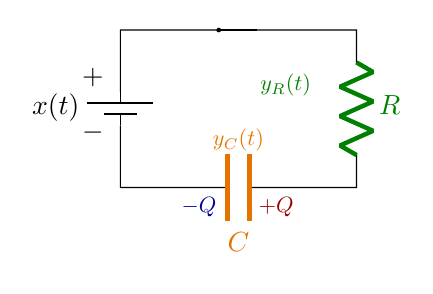
\begin{tikzpicture}
  \def\ang{220}
  \def\a{0.9}
  \def\b{0.8}
%   \draw[->,Icol] ({1.5+\a*cos(\ang)},{1+\b*sin(\ang)}) arc (\ang:-40:{\a} and {\b})
%   ;
  \draw (0,0) to[EMF] (0,2) --++(3,0)
              to[thick R] ++(0,-2) to[thick C] (0,0);
  \fill[black] (1.25,2) circle (0.03);
  \draw[line width=0.6] (1.25,2) --++ (0.48,0);
  \node at (-0.35,0.7) {$-$};
  \node at (-0.35,1.4) {$+$};
  \node[minuscol,scale=0.8] at (1.0,-0.25) {$-Q$};
  \node[pluscol,scale=0.8] at (1.98,-0.25) {$+Q$};
  \node[Ccol, scale=0.8] at (1.5,0.6) {$y_C(t)$};
  \node[Rcol, scale=0.8] at (2.1, 1.3) {$y_R(t)$};
\end{tikzpicture}

Circuit diff eq:
\[
    RC\Dot{y}_C(t) + y_C(t) = x(t)
\]

Let $x(t) = e^{i\omega t}\mapsto H_C(\omega) e^{i\omega t}$.

Therefore:
\[
    H_C(\omega) = \frac{\frac1{RC}}{i\omega + \frac1{RC}}
     = \frac{\frac1{RC}}{i\omega - \left(-\frac1{RC}\right)}
\]

This gives us a Low-Pass Filter with a peak at $\frac{\frac1{RC}}{\frac1{RC}}=1$ at 0 and a cutoff frequency of $\omega_c = -3dB=20\log_{10}\left(\frac1{\sqrt{2}}\right)$.

\begin{align*}
    \angle H(\omega)
    &= \angle \frac1{RC} - \angle \vec r
    \\
    &= \angle \frac1{RC} - \angle (i\omega + \frac1{RC})
    \\ 
    &= 0 - \angle (i\omega + \frac1{RC})
    \\
    &= -\arctan(\frac{\omega}{1/RC})
\end{align*}

Note: The phase of 0 is undefined.

\subsubsection{Impulse Response Revisited}
\[
    h_C(t) = \frac1{RC} e^{-\frac t{RC}} u(t)
\]

\[
    g(t) = \beta e^{-\alpha t} u(t) \iff G(\omega) = \frac{\beta}{i\omega + \alpha}
\]

\[
    h_C(t) = \frac1{RC} e^{-t/{RC}} u(t)
    \iff
    H_C(\omega) = \frac{\overbrace{1/{RC}}^\beta}{i\omega + \underbrace{1/{RC}}_{\alpha}}
\]

\hrulefill

\begin{align*}
    RC\Dot{y}_C(\tau) + y_C(\tau) &= x(\tau)
    \\
    RC \Dot{h}_C(\tau) + {h}_C(\tau)
    &= \delta(\tau)
    &&\text{[Note that this is the Dirac Delta]}
    \\
    RC \Dot{h}_C(\tau) e^{\tau/{RC}} + {h}_C(\tau) e^{\tau/{RC}}
    &= \delta(\tau) e^{\tau/{RC}}
    &&\text{[Mult. both sides by non-0 func $e^{\tau/{RC}}$]}
    \\
    &= \delta(\tau)
    \\
    \underbrace{\Dot{h}_C(\tau) e^{\tau/{RC}} + \frac1{RC} {h}_C(\tau) e^{\tau/{RC}}
    = \frac1{RC} \delta(\tau)}_{\dfrac{\mathrm d}{\mathrm d\tau}[h_C(\tau) e^{\tau/{RC}}]=\frac1{RC}\delta(\tau)}
    &= \frac1{RC}\delta(\tau)
    &&\text{[Product Rule of Differentiation]}
\end{align*}

\begin{shaded}
Note that we prefer integration over differentiation as differentiation is a numerically unstable operation when you have noise which comes hand-and-hand with analog systems.
\end{shaded}

\subsection{Integrator-Adder-Gain Block Diagram}
DAG Block: By FTC, we know to get rid of derivatives, we must integrrate!

\begin{align*}
    RC\Dot{y}_C + y_C &= x
    \\
    RC{y}_C + \int y_C &= \int x
    \\
    {y}_C = - \frac1{RC}\int y_C &+ \frac1{RC}\int x
\end{align*}

\subsection{CT-LTI Systems described by LCCDEs}
\subsection{RC-Ckt}
\subsection{Mass-Spring Damper}
See homework 5 q2.

    % \section{Tuesday, October 4th}
\subsection{Mass-Spring-Damp}
Note that you can have different matrices but they will be similar matrices (have the same eigenvalues).

\begin{align*}
    M\ddot y+D\dot y+Ky=x
    \\
    \dot q = \underbrace{\begin{bmatrix}0&1\\-\frac KM&-\frac DM\end{bmatrix}}_A \vec q+\begin{bmatrix}
        0\\
        \frac1M
    \end{bmatrix}
    x
    \\
    y = \underbrace{\begin{bmatrix}1&0\end{bmatrix}}_C \vec q
\end{align*}

\begin{align*}
    \det(\lambda I-A) = \lambda^2+\frac DM \lambda +\frac KM = 0
    \\
    \implies
    \lambda=-\frac D{2M}\pm\frac12\sqrt{\left(\frac{D}{M}\right)^2 - \frac{4K}{M}}
    \\
    \implies
    \lambda=-\frac D{2M}\pm\sqrt{\left(\frac{D}{2M}\right)^2 - \frac{K}{M}}
    \\
    \implies
    \lambda=-\frac D{2M}\pm\frac D{2M}\sqrt{1 - \frac{K}{M}\left(\frac{2M}{D}\right)^2}
\end{align*}

\hrulefill

Now we can look at cases: $D=0$
\begin{align*}
    \lambda = \pm\sqrt{-\frac KM}
    = \pm i\sqrt{\frac KM}= \pm i\omega
    \\
    \omega_0 = \sqrt{\frac{K}{M}}
    \\
    \left(\frac{D}{2M}\right)^2 - \frac KM = 0 
    \implies \lambda_1 = \lambda_2 = -\frac{D}{2M}
    \\
    \left(\frac{D}{2M}\right)^2 - \frac KM > 0 
\end{align*}
As you keep on increasing $D$, the 2 roots collide and collapse on $-\frac D{2M}$ which is a negative real number (on the negative x-axis).

\hrulefill

\begin{align*}
    \left(\frac{D}{2M}\right)^2 - \frac KM < 0 
    \\
    \implies \lambda_1, \lambda_2 \in\mathbb C
\end{align*}

\hrulefill

If we let 
\begin{align*}
    \lambda_1 = -\frac D{2M}+\frac D{2M}\sqrt{1 - \frac{K}{M}\left(\frac{2M}{D}\right)^2}
    &&\text{[This will be right of $\frac{-D}{2M}$ as we add sth $>0$ to a negative]}
    \\\lambda_2 = -\frac D{2M}-\frac D{2M}\sqrt{1 - \frac{K}{M}\left(\frac{2M}{D}\right)^2}
    &&\text{[This will be left of $-\frac{D}{2M}$ as we subtract from a negative]}
\end{align*}
This works due to the sqrt being strictly positive and less than 1 (due to being 1 minus some positive quantity).

We call it the overdamped case when we are to the left.

\hrulefill

Assuming we do not have the pathologically designed (Critically Damped) case of a single repeated eigenvalue then choosing our state vector to contain the \textbf{position} and \textbf{velocity}. Then we get
\[
    \dot q(t) = A q(t)
\]
or
\[
    q(t) = e^{At} q(0)
\]

So our initial position initial velocity are given by $q(0)$. Then 
\begin{align*}
    q(0) 
    &= 
    \alpha_1\vec v_1 + \alpha_2 \vec v_2
    \\
    \vec q(t) 
    &= 
    \alpha_1 e^{At} \vec v_1 + \alpha_2 e^{At} \vec v_2
    &&\text{[Note $e^{At}=\sum_{k=0}^\infty {t^kA^k}{k!}$]}
    \\
    &\implies e^{At}\vec v_1=e^{\lambda_1 t \vec v_1}
    &&\text{[Using the eigenfunction property]}
\end{align*}

\subsubsection{Purely Oscillatory}
\begin{align*}
    D=0\implies \lambda_1=i\omega_0, \lambda_2=-i\omega_0
    \\
    \vec q(t) = \alpha_1 e^{i\omega_0 t}\vec v_1+\alpha_2 e^{-i\omega_0 t}\vec v_2
\end{align*}

\hrulefill

Case when $\lambda_1 < 0, \lambda_2 < 0$ and $\lambda_1, \lambda_2\in\mathbb R$:

\begin{align*}
    q_1(t)
    &=\alpha_1 e^{\lambda_1 t}v_{11}+\alpha_2 e^{\lambda_2 t}v_{12}
\end{align*}

Another case is $\lambda_1=i\omega, \lambda_2=-i\omega$.

Note that complex eigenvalues come in conjugate pairs. So $\lambda = \sigma\pm i\omega_1$.
Note that $\sigma$ is a negative real scalar since eigenvalues need to be less than zero s.t. they decay.

\[
    \therefore q_1(t) = e^{\sigma t} \left[\alpha_1 e^{\lambda_1 t}v_{11}+\alpha_2 e^{\lambda_2 t}v_{12}\right]
\]

Therefore we get an oscillating decaying behavior.

\subsection{Interconnections of LTI Systems}
\subsubsection{Cascade Series}
\[
    x(t) \to \boxed{F} \to \boxed{G} \to y(t)
\]
is equivalent to 
\[
    x(t) \to \boxed{H} \to y(t)
\]
where $\boxed{H} := \boxed{\boxed{F} \to \boxed{G}}$

\begin{align*}
    h(t) &= (f \ast g)(t)
    &&\text{[As $F\to f(t)$]}
    \\
    x(n)\triangleq e^{i\omega t}
    \implies F \to F(\omega) e^{i\omega t}
    &\implies G \to G(\omega) F(\omega) e^{i\omega t}
    \\
    H(\omega) &= F(\omega) G(\omega)
\end{align*}
We have now found a property for series:
\begin{shaded}
    \[
        h(t) = (f \ast g)(t)
    \]
    \[
        H(\omega) = F(\omega) G(\omega)
    \]
\end{shaded}

\subsubsection{Parallel}
Likewise we can see that we get:
\begin{shaded}
    \begin{align*}
        h(t) &= (f + g)(t)
        \\
        H(\omega) &= F(\omega) + G(\omega)
    \end{align*}
\end{shaded}

\subsubsection{Feedback}
Given an LTI system with a feed-forward branch (Plant, $P(\omega)$) as well as a feedback branch (Controller, $K(\omega)$), find $H(\omega)$.

We know from the eigenfunction property that: $y(t)= H(\omega)e^{i\omega t}$.

Our input $x(t)\triangleq e^{i\omega t}$ tells us that:
\begin{align*}
    e^{i\omega t} + K(\omega)H(\omega)e^{i\omega t}
    \to 
    &\boxed{P(\omega)}
    \to P(\omega)\left[e^{i\omega t}
    +
    K(\omega)H(\omega)e^{i\omega t}\right]
    \\
    P(\omega)\left[1+ K(\omega)H(\omega)\right]\cancel{e^{i\omega t}}
    &=
    H(\omega)\cancel{e^{i\omega t}}
    &&\text{[$P(\omega) \to y(t)$]}
    \\
    H(\omega)
    &=
    \frac{P(\omega)}{1-K(\omega)P(\omega)}
\end{align*}

\subsubsection{Black's Formula:}
$H(\omega)=$ (Forward Gain)/(1 - Loop Gain)

\hrulefill

\[
    -60 \text{ dB}
    = 20\log_{10}\left(\frac{|\text{Out}|}{|\text{In}|}\right)
    \implies
    |\text{Out}|=\frac1{1000}|\text{In}|
\]

\hrulefill

What if we subtract $K(\omega)$ instead?


Then we get the new equation:
\[
    H(\omega)
    =
    \frac{P(\omega)}{1-(-K(\omega)P(\omega))}
    =
    \frac{P(\omega)}{1+K(\omega)P(\omega)}
    \approx
    \frac1{K(\omega)}
\]

Let $|K(\omega)P(\omega)|\gg1 
\ (\forall\omega\in[w_1, w_2])$ which is the frequency range of interest, we can then build flat $K(\omega)=K_0,$
 for $K_0<1$.
 
Note that here we assume the plant is stable -- which may not be necessarily true. If it is not the case then feedback can be used to stabilize it.

\subsection{Application 2: Inverse System Design}
I will title this after we get the main result.

Let us now reverse the roles of the controller and plant. We will also make this a ``negative feedback loop'' as we will subtract $P(\omega)$ as it goes into the adder with the input which this sum then goes through $K(\omega)$ to give us or output.

If $|K(\omega)P(\omega)|\gg1\ (\forall\omega\in[w_1, w_2])$ then:

\[
    H(\omega) = \frac{K(\omega)}{1+K(\omega)P(\omega)}
    \implies
    H(\omega) \approx \frac{\cancel{K(\omega)}}{\cancel{K(\omega)}P(\omega)}=\frac1{P(\omega)}
\]
This gives us an impulse response of $\delta$.

The title of this application is Inverse System Design.

\subsection{Application 3: Stabilization of Unstable Systems}
Given a voltage source connected to a Capacitor, we have:
\[
    y(t)=\frac1C\int_{-\infty}^t z(\tau)\mathrm d\tau
\]
\[
    h(t)=\frac1C\int_{-\infty}^t 
    \delta(\tau)\mathrm d\tau
    =\frac1C u(t)
\]

Is this absolutely integrable (e.g. $\int_{-\infty}^\infty |h(t)|\mathrm d t< \infty$)?\\
Note that the Capacitor is not BIBO-Stable.

Now with an RC circuit, realize that:
\[
    y(t)=\frac1C\int_{-\infty}^t z(\tau)\mathrm d\tau
    =\frac1C\int_{-\infty}^t \frac{x(\tau)-y(\tau)}{R}\mathrm d\tau
\]

The gain of $\frac1R$ acts like $K$ and the gain of $\frac1C$ composed with the integrator acts like $P$.

Conclusion: the RC circuit is actually \textit{a feedback system}.

    
    % \section{Tuesday, October 25th}
We started with the \textit{DTFS and DFT} which works for \textbf{periodic DT} signals.

Then we moved onto \textit{CTFS} which works for \textbf{periodic CT} signals.

Today we will look at the \textit{DTFT} which works for \textbf{aperiodic DT} signals.

Later we will look at the \textit{CTFT} which works for \textbf{aperiodic CT} signals.

\hrulefill

However we have some good news in store!

$h(n)$, which we define as either $h:\mathbb Z\to\mathbb R$ or $h:\mathbb Z\to\mathbb C$, can be written as $H(\omega)$ via \[H(\omega)=\sum_{n=-\infty}^\infty h(n)e^{-i\omega n}\]
which is exactly the DTFT of $h$.

Note that frequency responses will be $2\pi$-periodic instead of $p$-periodic and likewise $x\leftrightarrow H$ and $t\leftrightarrow \omega$.

\begin{align*}
    x(n) &= \frac1{2\pi}\int_{\langle2\pi\rangle} X(\omega) e^{i\omega n} \mathrm d \omega
    &&\text{[Synthesis Eqn.]}
    \\
    X(\omega) &= \sum_{n=-\infty}^\infty x(n) e^{-i\omega n}
    &&\text{[Analysis Eqn.]}
\end{align*}

\subsection{Method 2}
\begin{align*}
    x(t)=
    &\frac1{2\pi} \int_{\langle2\pi\rangle} X(\omega) e^{i\omega n} \mathrm d \omega
    &&\text{Note: can't have dirac delta on boundary}
    \\
    &\quad
    \langle2\pi\rangle
    =[\lambda,\lambda+2\pi]\quad\exists\lambda\in\mathbb R
    &&\text{uncountable set}
    \\
    x(n)
    &=\int_{\langle2\pi\rangle} \underbrace{\frac{\mathrm d \omega}{2\pi} X(\omega)}_{X_k \in \text{CTFT}} e^{-i\omega n}
    &&\text{Spectrum}
\end{align*}

\subsubsection{Method 2: Alternate Explanation}
Starting from:
\begin{align*}
    H(\omega)
    &=\sum_{n=-\infty}^\infty h(n) \underbrace{e^{-i\omega n}}_{\phi_n(\omega)}
    \\
    P_n(\omega) = e^{-i\omega n}
    \\
    H(\omega+2\pi)=H(\omega)\quad\forall\omega\in\mathbb R
    \\
    \phi_n(\omega+2\pi)=e^{-i(\omega+2\pi)n} = e^{-i\omega n} \cancelto1{e^{-i2\pi n}}
    \\
    H = \sum_n h(n) \phi_n
    \\
    \langle H,\phi_\ell\rangle
    =
    \langle \sum_n h(n)\phi_n,\phi_\ell\rangle
    &= 
    \sum_n h(n)\langle \phi_n,\phi_\ell\rangle
\end{align*}

\subsection{Inner Product Definition}
\begin{align*}
    \langle F, G\rangle 
    &\triangleq \int_{\langle2\pi\rangle} F(\omega)G^\ast(\omega)\mathrm d\omega
\end{align*}

\subsubsection{Method 2: Examples}
\begin{align*}
    \langle \phi_n, \phi_\ell \rangle 
    &\triangleq 
    \int_{\lambda}^{\lambda+2\pi} e^{-i\omega n} e^{i\omega\ell} \mathrm d\omega
    \\
    &=
    \int_{\lambda}^{\lambda+2\pi} e^{i\omega(\ell-n)} \mathrm d\omega
    \\
    &= 0 &&\text{after integration}
\end{align*}

Therefore
\begin{align*}
    \phi_n(\omega)
    &=e^{-i\omega n}
    \\
    \langle \phi_n, \phi_\ell \rangle 
    &= 2\pi\delta(n-\ell)
\end{align*}

\hrulefill

\begin{align*}
    % h(n) 
    % &= \frac1{2\pi} \int_{\langle2\pi\rangle}
    % \\
    \langle \phi_n, \phi_\ell \rangle  = 2\pi\delta(n-\ell)
\end{align*}

\subsection{Ideal lowpass filter}
Let us have a freq. response that is 2$\pi$-periodic which is centered at 0 which length $2B$.

\begin{align*}
    h(n)
    &=
    \frac1{2\pi} \int_{-\pi}^\pi H(\omega) e^{i\omega n} \mathrm d\omega
    \\
    &=
    \frac1{2\pi} \int_{-B}^B H(\omega) e^{i\omega n} \mathrm d\omega
    \\
    &=
    \frac1{2\pi} \int_{-B}^B A e^{i\omega n} \mathrm d\omega
    = \frac A{2\pi} \int_{-B}^B e^{i\omega n} \mathrm d\omega
    \\
    &=
    \frac A{2\pi}
    \left[-\frac{(i e^{i n \omega})}n\right]
    _{-B}^B
    \\&=
    \frac A{2\pi}
    \left(-\frac{(i e^{i n B})}n + \frac{(i e^{-i n B})}n\right)
    \\&=
    \frac A{n\pi}
    \left(\frac{e^{i n B} - e^{-i n B}}{2i}\right)
    \\
    h(n)
    &=
    \frac A{2\pi} \sin(Bn)
    &&\text{Note: Not causal}
\end{align*}

Note that $h\not\in\ell^1$ but $h\in\ell^2$ as decaying on the order of $\frac1n$ does not converge but decaying on the order of $\left(\frac1n\right)^2$ does converge so it is square summable.

Note that the DTFT, $X(\omega)$, will still be defined, just discontinuous -- so the analysis equation will not work, we would need to find the DTFT some other way. This is due to $X(\omega)$ being impulsive in nature -- it has dirac delta(s).

\subsection{Different Example}
\begin{align*}
    h(n)
    &\triangleq
    e^{i\omega_0n}\quad 0<\omega_0<\pi
    \\
    X(\omega)
    &= \dots
\end{align*}

Note that $h\not\in\ell^1$ and $h\not\in\ell^2$ as it does not converge.

\hrulefill

    % % % lec 17
\section{Thursday, October 27th}
\subsection{More DTFT Examples}
\subsection{Modulation Property}
\subsection{Circular Convolution}
\subsection{Rayleigh-Plancherel Identity}
\includepdf[pages=65-67]{lectures/img/EE_120_Notes_by_Jonny.pdf}

\includepdf[pages=68-70]{lectures/img/EE_120_Notes_by_Jonny.pdf}

    % % \include{./lectures/lecture19.tex}
    % % \include{./lectures/lecture20.tex}
    % % \include{./lectures/lecture21.tex}
    % % \include{./lectures/lecture22.tex}
    % % \include{./lectures/lecture23.tex}
    % % \include{./lectures/lecture24.tex}
    
    % %  \include{./lectures/lecture25.tex}
    
    % \section{Thursday, November 10th}
\subsection{Watching Video}
Here Professor Babak shows various Facebook videos that demonstrate the concept of aliasing to students.

Example: If your camera samples a video of a Helicopter at the same period (rate) that the propeller moves at then the Helicopter's propellers will appear to be stationary as the Helicopter seemingly hovers upwards.

\subsection{Sampling (Cont.)}
If time $\to Z$ transform

Then 
\[
    x_c(t) z(t) = x_z(t)
\]
where $z(t)=\sum_{-\infty}^\infty \delta(t-\ell T_s)$.

If we send $x_z(t)$ through a reconstruction (low-pass) filter with sampling frequency $\omega=\frac{2\pi}{T_s}$ then we can get $y_c(t)$.

Assuming Nyquist Criterion is met (no aliasing).

Today we will look at the time domain.
\begin{shaded}
Q: How do we get $h(t)$?
\end{shaded}
A: We can do use the synthesis equation:
\begin{align*}
    h(t)
    &=\frac1{2\pi}\int_{-\infty}^\infty X(\omega) e^{i\omega t} \mathrm d \omega
    \\
    &=\frac{T_s}{2\pi}\int_{-\omega_s/2}^{\omega_s/2} e^{i\omega t} \mathrm d \omega
    \\
    &=\frac{T_s}{2\pi}
    \left[
    \frac{e^{i\omega t}}{it}
    \right]_{-\omega_s/2}^{\omega_s/2}
    \\
    &=\frac{T_s}{\pi t}
    \sin\left(\frac{\omega_s t}{2}\right)
    \\
    &=\frac{T_s}{\pi t}
    \sin\left(\frac{\pi t}{2}\right)
    \\
    &=\frac{\sin\left(\frac{\pi t}{2}\right)}{\frac{\pi t}{T_s}}
    \\
    &=\text{sinc}\left(\frac t{T_s}\right)
    &&\text{[Normalized $\sin$]}
\end{align*}

which is $1$ at $t=0$.

We can confirm this with the synthesis equation:
\begin{align*}
    h(0) 
    &= \frac{T_s}{2\pi}\int_{-\omega_s/2}^{\omega_s/2}  \mathrm d \omega
    \\
    &= \underbrace{\frac{T_s}{2\pi}}_{\frac1{\omega_s}} \omega_s
    &&\left[\omega = \frac{2\pi}T\right]
    \\
    &= 1.\quad\square
\end{align*}

\hrulefill

\subsection{Sinc Interpolation}
\begin{align*}
    x_z(t) 
    &= x_c(t) \sum_{\ell=-\infty}^\infty \delta(t-\ell T_s)
    \\
    &=\sum_{\ell=-\infty}^\infty x_c(\ell T_s) \delta(t-\ell T_s)
    &&\text{[Sampling property of $\delta(\cdot)$]}
    \\
    y_c(t) 
    &= (x_z \ast h)(t)
    &&\text{[$(h\ast \delta_T)(t)=h(t-T)$]}
    \\
    &=\sum_{\ell=-\infty}^\infty x_c(\ell T_s) h(t-\ell T_s)
    &&\text{[$\delta_T(t)=\delta(t-T)$]}
    \\
    &=\sum_{\ell=-\infty}^\infty x_c(\ell T_s) 
    \underbrace{\frac{\sin\left[\frac{\pi(t-\ell T_s)}{T_s}\right]}{\frac{\pi(t-\ell T_s)}{T_s}}}_{\phi_\ell(t)}
\end{align*}

Note that linear, quadratic, etc interpolation also exist. However for the given reconstruction filter, we found that it can be represented as a linear combination of weighted sinc's.

Since the Nyquist criterion is met, the output of the reconstruction is the original signal (e.g. $y_c(t)=x_c(t)$).

To meet the Nyquist criterion, the sampling rate must be at least twice the frequency.

We're living in the space of CT-signals that are band-limited to $\frac{\omega_s}2$. In other words, we are looking at all non-zero signals i the range from $\omega=-\frac{\omega_s}{2}$ to $\omega=\frac{\omega_s}{2}$. This space is closed and satisfies the other properties to be a valid vector space. This vector space has a valid inner product which gives a valid geometry which tells us that the mutually orthogonal vectors (a proof of which is alluded to in homework) forms a bases.

\subsection{Rayleigh-Plancherel Identity}
\begin{align*}
    \langle \phi_\ell, \phi_k \rangle
    &=
    \frac{1}{2\pi} \langle \Phi_\ell, \Phi_k \rangle
    \\
    \phi_\ell(t) 
    &= \frac{\sin\left(\frac{\pi(t-\ell T_s)}{T_s}\right)}{\frac{\pi(t-\ell T_s)}{T_s}}
    \\
    \phi_0(t) 
    &= \frac{\sin\left(\frac{\pi t}{T_s}\right)}{\frac{\pi t}{T_s}}
    \\
    \Phi_\mathbf{\ell}(\omega)
    &=
    \Phi_0(\omega) e^{-i\omega \mathbf{\ell} T_s}
\end{align*}

If you sample at intervals of $T_s$, the value you get is the value of the original signal.

If you multiply by the unshifted sinc at 0 then you be 0 at $c\cdot T_s$ for all $c\in\mathbb Z \backslash \{0\}$. Note that at $0$, it will have value $\phi_0(t)$.

However this pattern holds generally for all $\phi_\ell(t)$, where only the sinc that is centered at $t=\ell T_s$ will be non-zero at the $T_s$ integer multiples. This is shown in the image below:
\begin{center}
    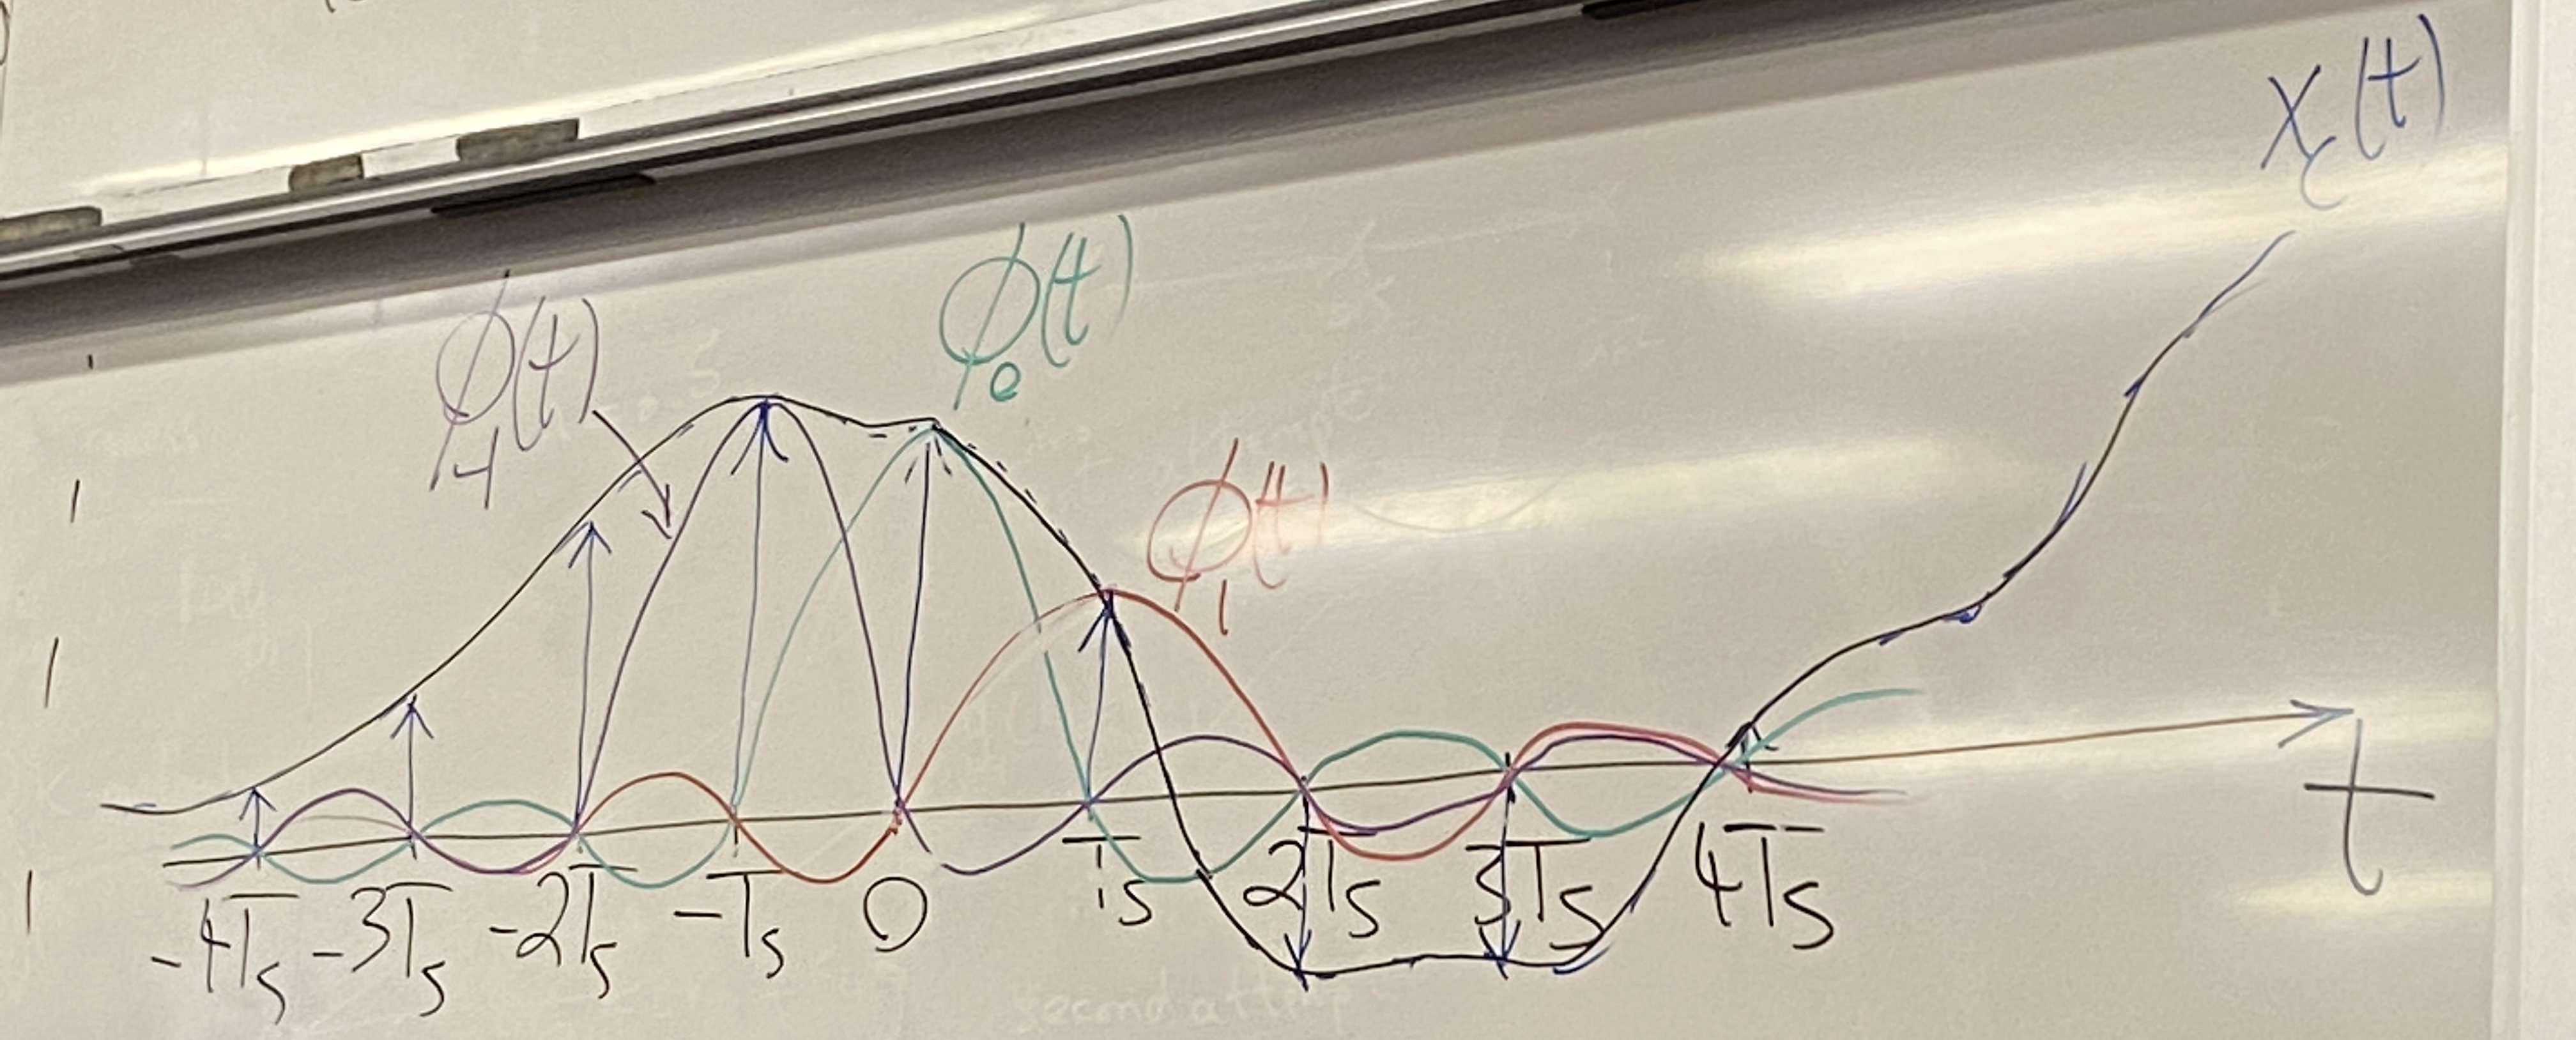
\includegraphics[scale=0.115]{lectures/wk11/img/sinc.jpg}
\end{center}

If $x\in$ space of signals bandlimited to $\frac{\omega_s}{2}$ then the $x_c(t) = \displaystyle\sum_{-\infty}^\infty x_c(\ell T_s)\phi_\ell(t)$.

$\{\phi_\ell(t)\}_{\ell=-\infty^\infty}$ form an orthogonal basis.

If you have taken EE 126 then you may know that $\langle X, Y\rangle \triangleq \mathbb E[XY]$. You can show this definition satisfies the least squares solution via the projection property.

\hrulefill

\subsection{Sampling Continued}
Note that the block diagram shown at the start of the class was not completed.

We know (from before):
\begin{align*}
    x_z(t) 
    &= x_c(t) \sum_{\ell=-\infty}^\infty \delta(t-\ell T_s)
\end{align*}
\begin{shaded}
But what is the transform?
\end{shaded}
\begin{align*}
    X_z(\omega) 
    &= \sum_{\ell} x_c(\ell T_s) \delta(t-\ell T_s)
    \\
    &=\sum_{\ell=-\infty}^\infty x_c(\ell T_s) \delta(t-\ell T_s)
    \\
    &=\sum_{\ell=-\infty}^\infty x_c(\ell T_s) \mathcal F\{\delta(t-\ell T_s)\}
    &&\left[\delta(t)\stackrel{\mathcal F}{\leftrightarrow}1\right]
    \\
    &=\sum_{\ell=-\infty}^\infty x_c(\ell T_s) e^{-i(\omega T_s)\ell}
    &&\left[\delta(t-\ell T_s)\stackrel{\mathcal F}{\leftrightarrow}e^{-i\omega\ell T_s}]\right]
    \\
    &=\sum_{\ell=-\infty}^\infty x_d(\ell) e^{-i(\omega T_s)\ell}
    \\
    &=
    X_d(\Omega)\Big|_{|\Omega = \omega T_s}
    &&\left[X_z(\omega)=X_d(\Omega)\Big|_{\Omega=\omega T_s}\right]
\end{align*}

We can note that the units work out:
\[
    \underbrace{\Omega}_{\text{rad/sample}} = \underbrace{\omega}_{\text{rad/sec}}
    \underbrace{T_s}_{\text{sec/sample}}
\]

\hrulefill
\subsection{Triangle Wave}

We can now look at a Triangle wave with period $2B$, centered at $0$.

Now we expand our horizon to the spectrum of $X_d(\Omega)$. Recall that $\Omega=\omega T_s$.

\begin{align*}
    X_z(\omega)
    &=
    X_d(\Omega)\Big|_{\Omega=\omega T_s}
    \\
    X_d(\Omega)
    &=
    X_z(\omega)\Big|_{\omega=\frac\Omega{T_s}}
    \\
    &=
    \frac1{T_s} X_c(\omega) \Big|_{\omega=\frac\Omega{T_s}},\quad|\Omega|\leq\pi.
\end{align*}

\begin{align*}
    Y_d(\Omega)
    &=
    Y_d(\Omega) H_d(\Omega)\quad |\Omega|\leq \pi
    \\
    &=
    \frac1{T_s} X_c(\omega) \Big|_{\omega=\frac\Omega{T_s}}H_d(\Omega)
\end{align*}

\hrulefill

Now we can send $y_d(n)$ and $T_r$ through a Kroneckor-to-Dirac block to get $y_z(t)=\displaystyle\sum_{\ell=-\infty}^\infty y_d(\ell)\delta(t-\ell T_r)$. 

Now we go from Lollipops to Diracs (the inverse of before). \textbf{Note that this step cannot possibly lead to any information loss.}

If we take the Fourier Transform of $y_z(t)$, we get $Y_z(\omega)$.

\begin{align*}
    Y_z(\omega)
    &=\sum_{\ell=-\infty}^\infty y_d(\ell) \mathcal F\{\delta(t-\ell T_r)\} \\
    &= \sum_{\ell=-\infty}^\infty y_d(\ell) e^{-i\omega\ell T_r} \\
    &= \sum_{\ell=-\infty}^\infty y_d(\ell) e^{-i(\omega T_r)\ell} \\
    &\therefore\quad Y_z(\omega)=Y_d(\Omega)\Big|_{\Omega=\omega T_r}
\end{align*}

which gives us the analysis equation for a DT signal!

Passing $y_z(t)$ through a low-pass filter yields $y_c(t)$.

\begin{align*}
    Y_c(\omega) 
    &= G Y_d(\Omega)\Big|_{\Omega=\omega T_r}
    &&\text{[Note the gain interpolates]}
    \\
    &= \frac G{T_s} X_c{\omega}\Big|_{\omega=\frac\Omega{T_s}=\frac{\omega T_r}{T_s}}
    H_d(\Omega)\Big|_{\Omega=\omega T_r}
    \\
    \therefore
    Y_c(\omega) 
    &= \frac G{T_s}X_c\left(\frac{\omega T_r}{T_s}\right) H\left({\omega T_r}\right)
\end{align*}

\hrulefill

\subsection{Overall System}

Overall, the final end-to-end system is the input $x_c(t)$ sent through a $C$-to-$D$ block with $T_s$ to get $x_d(n)$.

We then pass that into a $H_d(\Omega)$ to get $y_d(n)$ which we then pass through a $D$-to-$C$s block (with $T_r$) to get $y_c(t)$.

% Per req of Pei

\hrulefill

\subsection{LTI Equivalent Systems}
Note that although \textbf{sampling is not an LTI operation} (shifting the input will not lead to shifted sampled); however there is an LTI equivalent which has the frequency response $H_c(\omega)$.
\begin{align*}
    T_s = 
    &T_r = T
    \\
    Y_c(\omega) 
    &= \frac{G}{T} X_c(\omega) H_d(\omega T) 
    \\
    Y_c(\omega) 
    &= \frac{G}{T} H_d(\omega T) X_c(\omega)
\end{align*}

\subsection{Something fun to do}

\begin{align*}
    H_d(\Omega)
    &=1
    \\
    G
    &= 2T_s
    \\
    T_r
    &= 2T_s
    \\
    Y_c(\omega) 
    &= ?
    &&\text{[Want to find]}
    \\
    Y_c(\omega) 
    &=
    \frac G{T_s}X_c\left(\frac{\omega T_r}{T_s}\right) H\left({\omega T_r}\right)
    &&\text{[Eqn. from before]}
    \\
    Y_c(\omega) 
    &=
    2X_c(2\omega)
    \\
    \implies
    y_c(t) 
    &= 
    x_c(\frac t2)
\end{align*}
Here we compress in frequency which dilates in time.

This means that voice is at half the speed, half the pitch.

    % \section{Tuesday, November 15th}
\subsection{Z Transform}
Today we will learn about the Z Transform which is for discrete time signals. The counterpart for continuous time signals is the Laplace transform.

\subsubsection{Time to wean off the unit circle}
We know from before that passing $x(n)=e^{i\omega n}$ into an LTI system gives out $y(n)=H(\omega)e^{i\omega n}$.

\begin{shaded}
Q: What if we pass in $x(n)=z^n=(re^{i\omega})^n$ into an LTI system. What do we get then for $y(n)$?
\end{shaded}

Using the definition -- the exact same way we did for the purely imaginary case -- we can say that:
\begin{align*}
    y(n) 
    &=
    \sum_{\ell} h(\ell)x(n-\ell)
    \\
    x(n) = z^n
    &\implies
    x(n-\ell) = z^{n-\ell}
    \\
    \implies
    y(n) 
    &=
    \sum_{\ell} h(\ell) z^{n-\ell}
    \\
    &=
    \sum_{\ell=-\infty}^\infty h(\ell) z^{-\ell} z^n
\end{align*}

Note that the first part of $y(n)=\underbrace{\left(\sum_{\ell=-\infty}^\infty h(\ell) z^{-\ell}\right)}_{\hat H(z)} z^n$ is a function of nothing other than $z$. It is not a function of $\ell$ as we sum over all $\ell$. 

Therefore, we call $\hat H(z)$ the \textit{transfer function of the system}. You will often see this written as: $\displaystyle\hat H(z)= \sum_{n=-\infty}^\infty h(n)z^{-n}$

\hrulefill

Now we can complete what we were saying before:

Passing in $x(n)=z^n$ into an LTI system gives out $y(n)=\hat H(z)z^n$.\\
In other words: sending in a complex exponential into an LTI system gives the same complex exponential scaled by the transfer function.

\textbf{We call $\hat H(z)$ the Z Transform of $h(n)$.} Most texts will just say $H(z)$ but we add the hat to avoid confusion when talking about the DTFT (which are denoted as $H$) along with Z Transforms (which are denoted here as $\hat H$).

\subsection{Region of Convergence}
Note: we only define $\displaystyle\hat H(z)\triangleq\sum_{n=-\infty}^\infty h(n)z^{-n}\ $ \textbf{when the sum converges.}

Therefore we say that $z$ is in the Region of Convergence (ROC) if
\[
    \left|\sum_{n=-\infty}^\infty h(n)z^{-n}\right| < \infty
\]
Note that ROCs will always involve the absolute value of $z$.

\subsubsection{Aspects of Convergence}
\[
    z=re^{i\omega}
\]
\begin{shaded}
Q: Which aspect of $z$
\begin{itemize}
    \item $r$
    \item $\omega$
\end{itemize}
affects convergence?
\end{shaded}

The answer is $r$. $\omega$ does not affect convergence as it only exists within the term $e^{i\omega}$ which has magnitude 1. Or more rigorously:

\begin{align*}
    \left|\sum_\ell h(\ell)r^{-\ell}e^{-i\omega\ell}\right|&<\infty
    \\
    &\equiv
    \sum_\ell \left|h(\ell)r^{-\ell}\right|\left|e^{-i\omega\ell}\right|
    <\infty
    &&\text{[Magnitude of prod. = prod. of the magnitudes]}
    \\
    &\equiv
    \sum_\ell \left|h(\ell)r^{-\ell}\right|
    <\infty
    &&\text{$\left[|e^{-i\omega\ell}|=1\right]$}
\end{align*}

Note that the final expression $\sum_\ell \left|h(\ell)r^{-\ell}\right|<\infty$ has an $r$ in the LHS which appears in a potentially problematic manner:
if you have an impulse response that is growing, $r^\ell$ can contain the growth in the impulse response if chosen appropriately over an appropriate interval of $\ell$.

\subsubsection{Example of Convergence}
Let's give an example of choosing such an appropriate interval.

Say we have a causal system with $h(\ell)=2^\ell$. Then we can reformulate our condition to say that $\sum_{\ell=0}^\infty \left|(\frac 2r)^\ell\right|<\infty$, with the summation bounds following from causality. For this sum to converge, $\frac2r<1\implies r>2$. 
Taming choice example: If we take $r=3$, we will see that $\sum_{\ell=0}^\infty \left|(\frac 23)^\ell\right|<\infty$.

\subsubsection{Forms for Regions of Convergence}
Regions of Convergence can take on the following shapes, on the complex plane:
\begin{itemize}
    \item $R_0 < |z|$ (sometimes $R_0 < |z| <\infty$ to not include $z=\infty$): Regions of Convergence can be outside of some circle with radius $R_0$. Note that $R_0=0$ is possible in which case we include the entirety of the complex plane.
    \item $|z| < R_0$ (sometimes $0<|z|<R_0$ to not include $z=0$): Regions of Convergence can be inside of some circle.
    \item $R_0 < |z| < R_1$: the final possibility is if we have a donut.
\end{itemize}

\subsubsection{Duality of transforms of impulse responses}

Note that what we call the transfer function of the system is actually the Z transform of the impulse response.

Just like when we said that the frequency response of a system is the DTFT of the impulse response. 

\subsection{Why another Transform?}
Note there are signals that don't have a Fourier Transform (FT) but convolution is still well-defined.

We are familiar with the relationship (involving the DTFT) of sending in some $X(\omega)$ into a system $H(\omega)$ to get out $Y(\omega)=X(\omega)H(\omega)$. This however requires two things:
\begin{enumerate}
    \item the system, $H(\omega)$, has a frequency response
    \item the input has a DTFT
\end{enumerate}

However let us consider something new:\\
a system with impulse response $h(n)=2^n u(n)$ where your input is over a finite duration of 2 samples. Specifically $x(n)=\begin{cases}1 &\text{if n=0} \\ 2 &\text{if n=1} \\ 0 &\text{e/w} \end{cases}$.

We can see that convolution is well-defined here: $y(n)=\sum_{i=-\infty}^\infty h(i)x(n-i)=\begin{cases}1 &\text{n=0} \\ 2 &\text{n=1} \end{cases}$ \\
This is due to one of the signals being of finite length duration.

But you cannot talk about a FT since the system doesn't have a frequency response: \\
$H(\omega)=\sum_{n=0}^\infty 2^n e^{-i\omega n} =\sum_{n=0}^\infty (2 e^{-i\omega})^n$ but $|2 e^{-i\omega}|>1$ so the sum diverges for all $\ell_p$ norms $(\forall p)$. 
So while we do say that $h$ has no DTFT (so we can talk about the system in time -- via convolution -- but not in frequency), the system does turn out to have a Z Transform and so does the signal.

\subsection{Right-Sided Sequences}
\begin{shaded}
Definition:\\
We say a sequence $x$ is right-sided if $x(n)=0$ for all $n < N_0,\ \exists N_0 \in \mathbb Z$.
\end{shaded}
If we visualize a dot plot across $n$, then we will see that everything to the left of $N_0$ will be $0$ with lollipops only to the right.

In the case where $N_0=0$ then we are looking at a causal function.

\subsubsection{Convolution of 2 Right-Sided functions}
\begin{shaded}
Q: What if we have 2 right-sided signals $x, h$ and convolve them?
\end{shaded}

\[
    (x\ast h)(n) = \sum_{\ell=-\infty}^\infty x(\ell) h(n-\ell)
\]

We will have to keep one fixed (WLOG we shall keep $x(\ell)$ fixed here) and flip the other one (to get $h(-\ell)$) and then move it by some constant $n$ to get $h(n-\ell)$. \\
When we flip and move the \textit{right-sided} $h$, then everything non-zero moves from being to the right of some point $\ell=M_0$ to being only non-zero to the left of some different point $\ell=n-M_0$, with horizontal dotplot axes $\ell$. \\
Finally we multiply these 2 functions which leads to the following possible outcomes.\\
Either:
\begin{enumerate}
    \item $n-M_0$ (which is left-sided) is to the left $N_0$ (which is right-sided) in which case there is no overlap and the convolution \textbf{will yield 0.}
    \item Eventually as we increase $n$, the right-end of left-sided sequence will slide over the right-sided sequence and when we have overlap we will multiply pointwise.\\
    \textbf{This has finite overlap} due to the fact that they are extending in different directions and both sides have a stopping point $\Big(\ell=N_0$ for $x(\ell)$ and $\ell=n-M_0$ for $h(n-\ell)\Big)$.\\
    Finite overlap $\implies$ \textbf{finite output} once we've pointwise multiplied and summed.
\end{enumerate}
will occur.

\subsubsection{Example with Right-Sided functions}
\label{sec:ztransUnit}
Let's say you have some signal $x(n)=\left(\frac12\right)^n u(n)$. What is the Z Transform of this signal?\\
\textit{Hint: you will need to make use of $\ \displaystyle\sum_{n=0}^\infty \alpha^n =\frac{1}{1-\alpha},\quad |\alpha|<1$. \\Include constraints on $z$ for when the Z transform is defined: when its summation form converges.}
\begin{flalign*}
    \hat X(z) 
    &=
    \sum_{n=-\infty}^\infty x(n) z^{-n}
    &&\text{[Definition of Z Transform]}
    \\
    &=
    \sum_{n=-\infty}^\infty \left(\frac12\right)^n u(n) z^{-n}
    &&\text{[Plug in $x$]}
    \\
    &=
    \sum_{n=-\infty}^\infty \left(\frac1{2z}\right)^n u(n)
    &&\text{[Combine same exponential terms]}
    \\
    &=
    \sum_{n=0}^\infty \left(\frac1{2}z^{-1}\right)^n
    &&\text{[Use $z^{-1}$ notation, re-index per unit step]}
    \\
    &=
    \frac1{1-\frac12z^{-1}},\quad\left|\frac12z^{-1}\right|<1
    &&\text{[Use Hint; Introduce ROC constraints]}
    \\
    &=
    \frac1{1-\frac12z^{-1}},\quad|z|>\frac12
    &&\text{[Cleanup ROC constraints]}
\end{flalign*}

Therefore we can say that:
\begin{align*}
    x(n)=\left(\frac12\right)^n u(n)
    &\stackrel{\mathcal Z}\leftrightarrow 
    \hat X(z)=\frac1{1-\frac12z^{-1}},\quad R_x=\frac12<|z|
    \\
    x(n)
    &\stackrel{\mathcal Z}\leftrightarrow 
    \hat X(z)=\frac{z}{z-\frac12},\quad R_x=\frac12<|z|
    &&\left[\text{Multiply by $\frac zz$}\right]
\end{align*}

\subsection{Rational Z Transforms}
Note that this happens to be among the class of signals that have rational Z Transforms: This is rational in $z$ as it can be written as the ratio of 2 polynomials.

Roots of the numerator are called \textbf{zeros} of $\hat X$.\\
Roots of the denominator are called \textbf{poles} of $\hat X$.

In the above example, we have a zero at $z=0$ and a pole at $z=\frac12$.

We can give a pole-zero diagram by plotting the poles with X's and zeros with O's on the complex plane. ROCs are bounded by the poles as they can never include poles -- this is because poles are where things ``blow up'' as they are roots of the denominator. Zeros do not affect the ROC.

\subsection{DTFT Existence from Z Transforms}
In this case, we note that $ROC_x$ includes the unit circle which tells us that the DTFT exists:
Recall that we define
\begin{align*}
    \hat X(z)&=\sum_n x(n)z^{-n}
    \\
    &=\sum_n x(n)r^{-n} e^{-i\omega n}
    &&[z=re^{i\omega}]
\end{align*}
But if $r=1$ is inside the ROC then the above summation converges -- as then $z=e^{i\omega}$ is just somewhere \textbf{on} the unit circle. We will also notice that the $X(\omega)=\sum_n x(n) e^{-i\omega n}$ is the analysis equation for the DTFT as we plug in $r=1$.

More formally:
\[
    x(n)=\left(\frac12\right)^n u(n)
    \stackrel{\mathcal F}\leftrightarrow 
    \hat X(z)\left.\right|_{z=e^{i\omega}}=\frac1{1-\frac12e^{-i\omega}}
\]
which we will recall from our Fourier Transform days.

Note that we can only say $\hat X(z)\left.\right|_{z=e^{i\omega}}=X(\omega)$ if the ROC includes the unit circle.

\subsection{Z Transforms \texorpdfstring{$\to$}{->} DTFT Example}
\subsubsection{Z Transform with incorrect DTFT}
Let us find the Z Transform and then convert it into the DTFT for the signal $x(n)=u(n)$.

\begin{flalign*}
    \hat X(z) &= \sum_n u(n) z^{-n}
    &&\text{[Definition of Z Transform]}
    \\
    \hat X(z) &= \sum_{n=0}^\infty z^{-n}
    &&\text{[Re-index summation bounds per unit step]}
    \\
    \hat X(z) &= \sum_{n=0}^\infty (z^{-1})^n
    &&\text{[Introduce $z^{-1}$ term]}
    \\
    \hat X(z) &=\frac1{1-z^{-1}},\quad R_x = |z^{-1}|<1
    &&\text{[Geometric Series Convergence]}
    \\
    \hat X(z) &=\frac z{z-1},\quad R_x = 1<|z|
    &&\text{[Multiply by $\frac zz$ to find zeros/poles]}
\end{flalign*}

So we have a zero at $z=0$ and a pole at $z=1$, so our ROC extends outwards from the unit circle; however, it does not include the unit circle. \\
So \textbf{we cannot say} $X(\omega)=\frac1{1-e^{i\omega}}$ (in fact this is not the transform of the unit step function as $u(n)\not\in\ell_1, u(n)\not\in\ell_2, u(n)\in\ell_p \implies$ DTFT must have dirac deltas which we do not have).

\subsubsection{Correct DTFT}
The correct DTFT transform is
\[
    X(\omega)=\frac1{1-e^{-i\omega}}+\pi\delta(\omega),\quad \forall(|\omega|<\pi)
\]
with $2\pi$ periodicity. Note that $\frac12\stackrel{\mathcal F}\leftrightarrow \pi\delta(\omega)$ with normalization=1, oscillatory factor=-1 if you wish to verify with WolframAlpha.

We can wrap the $2\pi$-periodicity in one expression as:
\[
    X(\omega)=\frac1{1-e^{-i\omega}}+\pi\sum_{\ell=-\infty}^\infty\delta(\omega-2\pi\ell),\quad \forall\omega
\]


\subsection{Inverse Transforming}
\begin{important}
Note that there is an inverse Z Transform that we are going to treat as radioactive as it requires immense knowledge of Complex Analysis, Contour Integration, etc.
\end{important}
Therefore the inverse transforming that we do -- for both Z Transforms as well as Laplace Transforms -- will be limited to transform properties and known Z transform pairs.

\hrulefill

\subsection{Same but Different Z Transforms}
Given $q(n)=-\left(\frac12\right)^n u(-n-1)$, we know that $q(n)$ is non-zero for $-n-1\ge0$ or $n\le-1$. This is important to take care of as otherwise the unit step function will make $q=0$. Therefore it is non-zero for the first time at $n=-1$, with value $q(-1)=-2$ or $q(-1)=-\left(\frac12\right)^{-1}$. Then at the next time step $n=2$, we will maintain our negative sign but we shall grow our magnitude to have $q(-2)=-\left(\frac12\right)^{-2}$. And for all future negative timesteps, $q$ will continue to grow \textbf{exponentially}.

Since the $q$ is of exponential growth, we know that there will be no DTFT. This means that the $\text{ROC}_q$ must not include the unit circle. 
Finding the Z Transform:

\begin{flalign*}
    \hat Q(z)
    &=
    -\sum_{n=-\infty}^{-1} \left(\frac12\right)^n z^{-n}
    &&\text{[Re-index summation per modified unit step]}
    \\
    &=
    -\sum_{\ell=1}^{\infty} \left(\frac12\right)^{-\ell} z^{\ell}
    &&\text{[Change of variables: $\ell=-n$]}
    \\
    &=
    -\sum_{\ell=1}^{\infty} (2z)^{\ell}
    = -\left(\sum_{\ell=0}^{\infty} (2z)^{\ell} - 1\right)
    &&\text{[Combine, re-index]}
\end{flalign*}

This means we have 
\begin{align*}
    \hat Q(z) &= \frac{2z}{2z-1},\quad|z|<\frac12
    \\
    \hat Q(z) &= \frac{1}{1-\frac12 z^{-1}},\quad|z|<\frac12
\end{align*}
for our Z Transform, with the ROC being the exclusive circle extending inwards of radius $\frac12$.

Combining \hyperref[sec:ztransUnit]{with the earlier found Z transform\{u(n)\}}, we get that:
\begin{align*}
    \frac1{1-\frac12z^{-1}} \stackrel{\mathcal Z}\leftrightarrow
    \begin{cases}
        \left(\frac12\right)^n u(n) & \text{ if } |z| > \frac12
        \\
        -\left(\frac12\right)^n u(-n-1) & \text{ if } |z| < \frac12
    \end{cases}
\end{align*}
Note that the first case is stable -- as it contains the unit circle -- while the latter is not.

Looking at the pole-zero diagram, we see that the diagram is the same: \\
either way we have a zero at $z=0$ and a pole at $z=\frac12$. However the ROCs are different.

\subsection{ Generalizations from Causality to left/right-sided}
\begin{center}
    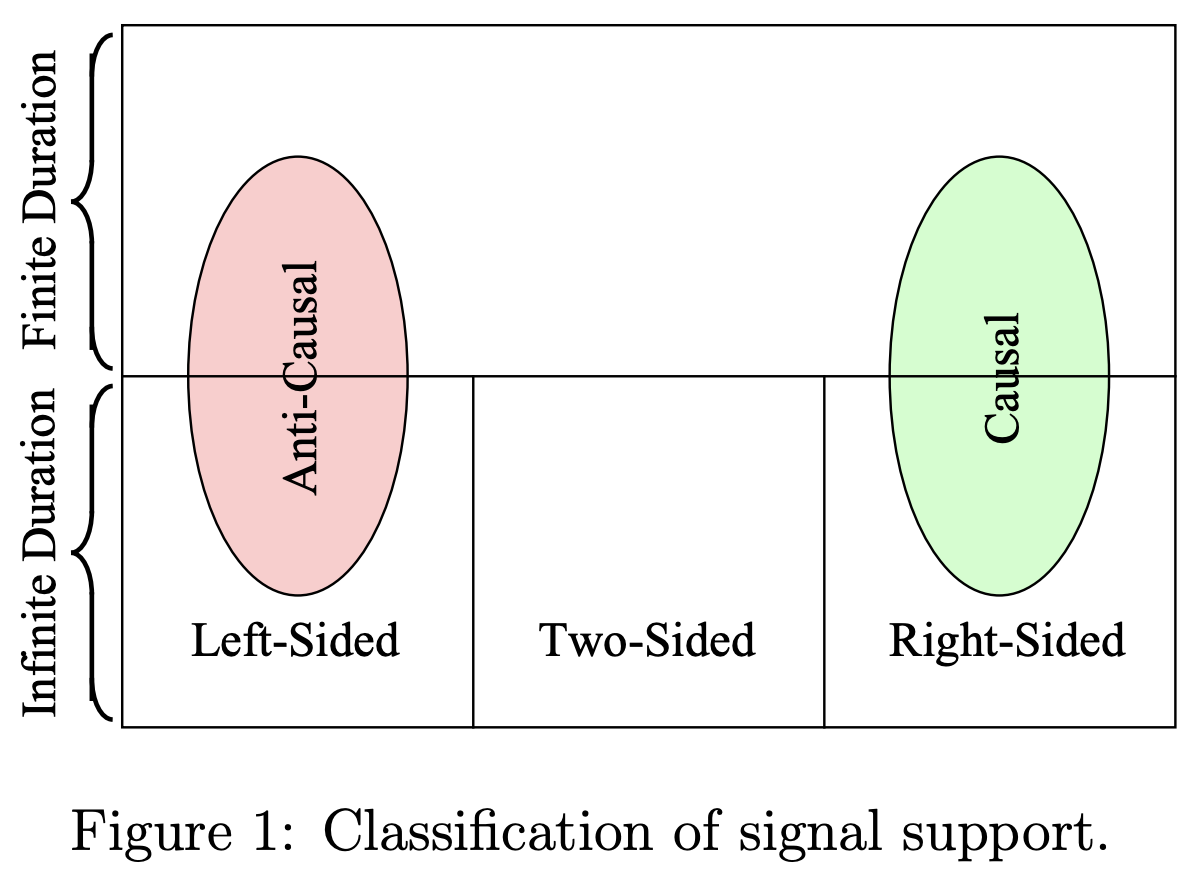
\includegraphics[scale=0.25]{lectures/wk12/img/signal_classification.png}
\end{center}

where an Infinite Right-sided Signal is Causal if the ROC includes $\infty$ and likewise for a Left-sided signal and the origin.

\subsubsection{Proof of Causal Extending}
For some causal signal $x(n)$ we know that any $R_1\in\text{ROC}_x$ will make the Z Transform converge by definition of the ROC (Region of Convergence). \\
Likewise since $R_1$ is in the ROC, we know it must be greater than the outermost.

So if
\[
    \hat X(R_1 e^{i\omega}) = \sum_{n=0}^\infty x(n) R_1^{-n} e^{-i\omega n}
\]
converges, then we know that \textit{any $R_2$} such that $R_2 > R_1$ will only make the summation converge faster. We can induct upon this idea and see there is no outer boundary to the radius.\\
$\therefore \hat X(R_2 e^{i\omega})$ certainly converges: if $R_1$ makes the sum converge then $R_2$ can too.

\subsubsection{Relationship between Time and Transform}
Note that the outermost pole is the pole that decays fastest and the ``dominant poles'' are the ones that decay slowest -- the ones that are away from the boundary. 

\subsubsection{Non-Causal Right-sided signals}
An example of such a signal lies within some signal $y(n)=\left(\frac12\right)^{n+1} u(n+1)=x(n+1)$. We can see that this signal $y$ starts at $n=-1$ and then for all future timesteps ($n=0,1,2,\ldots$), we see $y$ decay.

Finding the Z Transform:
\begin{align*}
    \hat Y(z) 
    &= \sum_{n=-1}^\infty y(n) z^{-n} 
    \\
    &= \underbrace{z}_{y(-1)(z^{-1})^{-1}} + \underbrace{\frac12}_{y(0)(z^{-1})^{0}}
    + \ast z^{-1} + \square z^{-1} + \cdots
\end{align*}
where the $\ast$ and $\square$ coefficient terms are irrelevant garbage.

As $z\to\infty$, the first term blows up. Even though we have a right-sided signal, the very first term (aka one lollipop on the dotplot which causes problems) leads to us not being causal.

Therefore the ROC$_y = \frac12<|z|<\infty$ where we exclude infinity to denote that we are not causal.

\subsubsection{Anti-Causal and Left-sided signals}
If you have an anti-causal signal you grow inwards including the origin.

But left-sided signals that are not anti-causal go all the way to the origin but do not include it.

You will see more nuances of this in the homework: problem set 10.

\subsection{ RoC Causality and Left/Right-sidedness Summary}
\begin{itemize}
    \item Causal RoC: $R_0<|z|$
    \item Right-sided but not causal RoC: $R_0<|z|<\infty$
    \item Anti-causal RoC: $|z|<R_0$
    \item Left-sided but not anti-causal RoC: $0<|z|<R_0$
\end{itemize}
\begin{shaded}
Q: Is the exclusion of 0 important as it means the constant signals cannot be included?
\end{shaded}
A: No, constant signals are $|z|=1$.

\subsubsection{Anti-Causality vs Non-Causality}
Anti-Causal ($h(n)=0,\forall n>0$) is always one-sided 
whereas non-causal can also be two-sided (donut shaped RoCs).

\subsection{ Mixing Z Transforms}
Anytime you mix Z Transforms, you have to make sure the RoCs have a non-trivial overlap.\\
Otherwise, one or the other is not convergent.

\subsubsection{Mixing Z Transforms Example}
\begin{align*}
    x(n)
    &=\left(\frac12\right)^n u(n) - 2^nu(-n-1)
    \\
    x(n)
    &\stackrel{\mathcal Z}\leftrightarrow
    \frac1{1-\frac12z^{-1}} + \frac1{1-2z^{-1}}
    \\
    \text{ROC}&=\quad\frac12<|z|\ \cap\ |z|<2
    \\
    \hat X(z)
    &=\frac z{z-\frac12} + \frac z{z-2}
    \\
    &=\frac{2z(z-\frac54)}{(z-\frac12)(z-2)}
    &&\text{[Common denominator $\to$ factor]}
    \\
    \text{ROC}&=\quad\frac12<|z|<2
\end{align*}

This is a non-causal (or 2-sided) decaying exponential signal.

\begin{shaded}
Sanity Check: Since each of the 2 parts of $x(n)$ is absolutely summable (as they are decaying exponentials), we know that the ROC must include the unit circle which it does!
\end{shaded}

\subsection{ Convolution in Time}
Let us feed in $x(n)=z^n$ to system $h(n)$ (which internally is a composition of $f(n)$ sent into a $g(n)$) to get out $y(n) =\hat H(z)z^n$.

This means that $z^n$ is also an eigenfunction of an LTI system, just like $e^{i\omega}$ was but now you are not restricted to being on the unit circle.

Breaking it down, step-by-step, we see that:\\
$f(n)$ gives out $\hat F(z)z^n$\\
which is sent to $g(n)$ which gives out $y(n)=\hat F(z)\hat G(z) z^n$.

Pattern matching to before, we see that $\hat H(z)=\hat F(z)\hat G(z)$.

\begin{shaded}
Big idea: Convolution in Time $\mapsto$ Multiplication in the Transform domain (just like with FT).
\end{shaded}

\subsection{ Generalization of Convolution in Time}
If we pass $x(n)$ into a system $h(n)$ to get $y(n)=(x\ast h)(n)$.

Then $\hat Y(z) = \hat X(z)\hat H(z)\implies \hat H(z)=\frac{\hat Y(z)}{\hat X(z)}$.

\subsection{ Time-Shift Property}
For a signal $x(n)$ with a Z Transform, let us define $y(n)\triangleq x(n-N)$.

This shall have Z Transform: $\hat Y(z)=\hat X(z)z^{-N}$ which you know from you incredible EE120 Prof!
\begin{align*}
    \hat Y(z)
    &= \sum_{n} x(n-N) z^{-n}
    &&\text{[Definition of Z Transform]}
    \\
    &= \sum_{\ell} x(\ell) z^{-(\ell+N)}
    &&\text{[Change of Variables: $\ell=n-N\implies n=\ell+N$]}
    \\
    &= \sum_{\ell} x(\ell) z^{-\ell} z^{-N }
\end{align*}
This is why we saw delay blocks written as $z^{-1}.\hfill\square$

    % \section{Thursday, November 17th}
\subsection{Z Transform (Continued)}
Today we will continue our journey through the Z Transform.

Last time we ended with the Time-Shift Property:
\begin{align*}
    x(n) &\zt \Xhat
    \\
    x(n-N) &\zt \zN\Xhat
\end{align*}

If $N>0$, then the RHS of the 2nd line can be written as $\to\frac\Xhat\zpN$.
\begin{important}
Q: What could potentially go wrong?
\end{important}
A: You could have a pole at $z=0$, which gets canceled out with the numerator thus leading to the loss of a solution -- note that this depends on what $\Xhat$ is.

If $N<0$, then we could potentially lose $\infty$ from the RoC.\\
Example $N=-1$: $u(n+1)\zt\frac{z^2}{z-1},\quad1<|z|<\infty$ where we exclude $z=\infty$ as we diverge there.

\hrulefill

\subsection{Time-Reversal Property}
Given $x(n)\zt\Xhat=\displaystyle\sum_n x(z)\zn$, let us define the time reversed $x$ as $x_{\text{TR}}(n)\triangleq x(-n)$. \\
Find the Z Transform of $x_{\text{TR}}(n)$.
\begin{align*}
    \Xshat{TR} 
    &= \sum_n x(-n)\zn
    \\
    &= \sum_\ell x(\ell)\zpl
    &&\text{[Change of Variables: $\ell=-n$]}
    \\
    &= \sum_\ell x(\ell)(\zinv)^{-\ell}
    \\
    &=\Xphat{\zinv}
\end{align*}

Let us say that the ROC for $x$ is $R_x=\{z\in\mathbb C\ \Big|\ r_1<|z|<r_2\}$.

Then $R_{x_{\text{TR}}} = \{z\in\mathbb C\ \Big|\ r_1<|z^{-1}|<r_2\}
= \{z\in\mathbb C\ \Big|\ \frac1{r_1}<|z|<\frac1{r_2}\}$.

Graphically we can see that the pole-zero plots of $x(n)$ as well as that of $x_{\text{TR}}(n)$ are both two-sided.

\subsection{Multiplication by a complex expon.}
Given $x(n)\zt\Xhat=\displaystyle\sum_n x(z)\zn$, let us define the signal $q(n)\triangleq\zopn x(n)$. \\
Find the Z Transform and RoC of this signal.
\begin{align*}
    \hat Q(z) 
    &= \sum_n \zopn x(n)\zn
    \\
    &= \sum_n x(n)\left(\frac{z}{z_0}\right)^{-n}
    \\
    &= \Xphat{\frac{z}{z_0}}
\end{align*}
where $z_0=r_0e^{i\omega_0}$.

Since $R_x=\{z\in\mathbb C\ \Big|\ r_1<|z|<r_2\}$,

we have $R_{q} = \{z\in\mathbb C\ \Big|\ r_1<\left|\frac{z}{z_0}\right|<r_2\}
= \{z\in\mathbb C\ \Big|\ r_1<\frac{|z|}{r_0}<r_2\}
= \{z\in\mathbb C\ \Big|\ {r_0}r_1<{|z|}<{r_0}r_2\}$.

Note that if $|z_0|>1$ then you will have an \textbf{expansion} between the two circles that the RoC sits.

Note that if $|z_0|<1$ then you will have a \textbf{contraction} between the two circles that the RoC sits.

\subsection{Suddenly-Applied Sinusoidal Excitation}
Find the Z Transform of $r(n)=\cos(\omega_0 n) u(n)$.

We can start by actually simplifying: $r(n)=\cos(\omega_0 n) u(n) = \frac12e^{i\omega_0 n}u(n)+\frac12e^{-i\omega_0 n}u(n)$.

If we let $z_0=e^{i\omega_0}$, we can use the fact that $u(n)\zt \hat U(z)=\frac{z}{z-1},\quad1<|z|$\\
as well as the fact that $q(n)=\zopn x(n)\zt \hat Q(z)=\Xphat{\frac{z}{z_0}}$,\\
we can then realize $z_0^n u(n)
=e^{i\omega_0n}u(n)
\zt
\hat U\left({\frac{z}{z_0}}\right)
=\hat U\left({\frac{z}{e^{i\omega_0}}}\right)
=\frac{\frac{z}{e^{i\omega_0}}}{\frac{z}{e^{i\omega_0}}-1}
=\frac{{e^{-i\omega_0}{z}}}{{e^{-i\omega_0}{z}}-1}$.\\
Likewise, $z_0^{-n} u(n)
=e^{-i\omega_0n}u(n)
\zt
\hat U\left({\frac{z}{e^{-i\omega_0}}}\right)
=\frac{{e^{i\omega_0}{z}}}{{e^{i\omega_0}{z}}-1}$
\begin{align*}
    \hat R(z) 
    &=
    \frac12
    \left[
        \frac{{e^{-i\omega_0}{z}}}{{e^{-i\omega_0}{z}}-1}
        +
        \frac{{e^{i\omega_0}{z}}}{{e^{i\omega_0}{z}}-1}
    \right]
    \\
    &=
    \frac12
    \left[
        \frac{{{z}}}{{{z}}-e^{i\omega_0}}
        +
        \frac{{{z}}}{{{z}}-e^{-i\omega_0}}
    \right]
    &&\text{[Multiply by $\pm\frac{e^{i\omega_0}}{e^{i\omega_0}}$]}
    \\
    &=
    \frac{z}2
    \left[
        \frac{1}{{{z}}-e^{i\omega_0}}
        +
        \frac{1}{{{z}}-e^{-i\omega_0}}
    \right]
    &&\text{[Pull the $z$ out]}
    \\
    &=
    \frac{z}2
    \left[
        \frac{z-e^{-i\omega_0} + z-e^{i\omega_0}}{(z-e^{i\omega_0})(z-e^{-i\omega_0})}
    \right]
    &&\text{[Common Denominator]}
    \\
    \hat R(z) 
    &=
    \frac{z(z-\cos(\omega_0))}{(z-e^{i\omega_0})(z-e^{-i\omega_0})}
    &&\left[\cos(\omega_0)=\frac{e^{i\omega_0}+e^{-i\omega_0}}{2}\right]
\end{align*}
The Pole-Zero diagram will have zeros at $z=0, \cos(\omega_0)$ and poles on the unit circle at $z=e^{i\omega_0}, e^{-i\omega_0}$, one rotated by an angle of $+\omega_0$ and the other rotated by $-\omega_0$.\\
Note that this statement assumes that $\omega_0$ is positive.

Because this system is causal, the RoC will extend outwards form the unit circle.

\begin{shaded}
Note that if $z=\xi_0$ is a zero of the original function, now $\frac{z}{e^{i\omega_0}}=\xi_0$ is a zero of $z=\xi_0e^{i\omega_0}$.
\end{shaded}

\subsection{Uniqueness of the Z Transform}
If you are told that the Z Transform is rational then it is unique up to a constant factor, $H_0$:
\begin{equation}\label{eq:ratzt}
    \hat H(z) 
    = H_0 \frac{\displaystyle\prod_{x_i\in Z} (z-x_i)}{\displaystyle\prod_{p\in P} (z-p)}
\end{equation}
where $Z$ is the set of zeros and $P$ is the set of poles. 

In the homework, you shall work with this much more. If I tell you that the DC Gain of a Filter is $1$, you know that the transfer function $\hat H(z)\left.\right|_{z=1}=1$ as $e^{i0}=1\zt z=1$. Then you can solve for the constant $H_0$ by setting \eqref{eq:ratzt}, evaluated at the DC Gain, to 1.

\subsection{DT-LTI System Example Questions}
Consider a DT-LTI filter ${H}$ that is causal and has a rational $\hat H(z)$, with\\ 
$x(n)=1 \to \boxed{H} \to y(n)=-\frac{4}{3}$. 

The pole-zero diagram has poles at $z=-\frac{1}{2}, \frac{3}{4}$, and a zero at $z=\frac{3}{2}$. 
\begin{shaded}
Questions:
\begin{enumerate}
    \item Warmup: Is H BIBO stable?
    \item What is $\hat{H}(z)$ (and then find $h(n)$ from it).
\end{enumerate}
\end{shaded}
Answers:
\begin{enumerate}
    \item First let us find the RoC. Since $H$ is causal (or right-sided), we know that the RoC extends outwards from the outer most pole.
    This leads to $R_h=\{z\in\mathbb C\Big|\frac34<|z|\}$.
    Therefore we know $H$ is BIBO stable as the unit circle is included in the RoC.
    \item $\hat{H}(z)=A\frac{z-\frac32}{(z+\frac12)(z-\frac34)},\quad\frac34<|z|$ where $A$ is some scaling factor.
\end{enumerate}

\subsubsection{Finding the Unique Z Transform}
We can find $A$ using the fact that $x(n)=1=\zopn\to\boxed{H}\to y(n)=-\frac43$ is analogous to:\\
$x(n)=\zopn\to\boxed{\Hhat}\to y(n)=\Hphat{z_0}\zopn$.

$x(n)=1=z_0^n$ for $z_0=1$, therefore $\hat{H}(1)=-\frac{4}{3}$. 
\begin{align*}
    \hat{H}(z)
    &=A\frac{z-\frac32}{(z+\frac12)(z-\frac34)}
    &&\text{[Original Z Transform]}
    \\
    \hat{H}(1)
    &=A\frac{1-\frac32}{(1+\frac12)(1-\frac34)} = -\frac43
    &&\text{[Plug in $z=1$ to use the known value of $\hat{H}(1)$]}
    \\
    -\frac43
    &=
    A\frac{1-\frac32}{(1+\frac12)(1-\frac34)} = -\frac{4A}3
    \\
    \frac{4A}3 &= \frac43
    \implies
    \boxed{A = 1}
\end{align*}

\subsubsection{Finding the Impulse Response}
Let us simplify the task of finding $h(n)$, let us start by finding $h(0)$.

Here's a hint to do so:
\begin{flalign*}
    \Hhat 
    &=\sum_{n=0}^\infty h(n) z^{-n}
    &&\text{[Definition of Z Transform for Causal System]}
    \\
    \Hhat 
    &= h(0) + h(1) \zinv + h(2)\ze{2} + \cdots
    \\
    \implies
    \lim_{z\to\infty}\Hhat 
    &= h(0)
    &&\text{[Zero out all the terms after $h(0)$]}
    \\
    \lim_{z\to\infty}\Hhat 
    &= 0
    &&[\text{order}(\text{denom}\{\hat H\})>\text{order}(\text{numer}\{\hat H\})]
\end{flalign*}
as $\text{order}(\text{denominator}\{\Hhat\})=2,\ \text{order}(\text{numerator}\{\Hhat\})=1$ and $2>1$.

\subsection{Initial Value Theorem}
\begin{shaded}
If a signal or function $h$ is causal -- if $h(n)=0, n<0$ -- then we can find the initial value as such: $\displaystyle\lim_{z\to\infty}\Hhat=h(0)$.
\end{shaded}
Note that casual is a term for systems so we are currently abusing terminology -- we simply mean that the signal is $0$ on the left-side of the origin.

\subsection{Impulse Response from a Z Transform}
To find $h(n)$, we will need to revisit our Calculus days to utilize Partial Fraction Decomposition:
\begin{align*}
    \hat{H}(z)
    =\frac{z-3 / 2}{(z+1 / 2)(z-3 / 4)}
    &=\frac{\alpha}{z+1 / 2}+\frac{\beta}{z-3 / 4}
    \\
    =\frac{z-3 / 2}{(z+1 / 2)(z-3 / 4)}
    &=\frac{(\alpha+\beta)z+(\frac\beta2-\frac{3\alpha}{4})}{(z+1 / 2)(z-3 / 4)}
    &&\text{[Common Denominator]}
    \\
    &\implies
    \alpha+\beta=1,\ \frac\beta2-\frac{3\alpha}{4}=-\frac32
    &&\text{[Pattern-match like-terms]}
    \\
    &\implies
    \alpha=\frac85, \ \beta=-\frac35
    &&\text{[Solve the system]}
\end{align*}

Therefore,
\begin{align*}
    \hat{H}(z)
    &=\frac{8}{5} \frac{1}{z+\frac{1}{2}}
    &&-\frac{3}{5} \frac{1}{z-\frac{3}{4}}
    &&&\text{[PFD form with respective $\alpha,\beta$]}
    \\
    &=\frac{8}{5}\zinv\left(\frac{z}{z-\frac{-1}{2}}\right) 
    &&-\frac{3}{5}\zinv\left(\frac{z}{z-\frac{3}{4}}\right)
    \\
    h(n)
    &=\frac{8}{5}\zinv\left(-\frac{1}{2}\right)^{n} u(n)
    &&-\frac{3}{5}\zinv\left(\frac{3}{4}\right)^{n} u(n)
    &&&[\dagger: \lambda_1=-\frac12, \lambda_2=\frac34]
    \\
    h(n)
    &=\frac{8}{5}\left(-\frac{1}{2}\right)^{n-1} u(n-1)
    &&-\frac{3}{5}\left(\frac{3}{4}\right)^{n-1} u(n-1)
    &&&\text{[Delay by one sample]}
\end{align*}
$^\dagger$ as $\lambda^n u(n)\zt \frac1{1-\lambda\zinv}=\frac{z}{z-\lambda},\quad|\lambda|<|z|$.

Sanity Check: $h(0)=0$ is satisfied -- due to the unit step functions!

\subsection{Differentiation in \texorpdfstring{$z$}{z}}
Given $x(n)\zt \Xhat$, show that $nx(n)\zt -z\dv{\Xhat}{z}$.
\begin{align*}
    \Xhat 
    &= \sum_n x(n)\zn
    \\
    \dv{\Xhat}{z} 
    &= -\sum_n n x(n) \ze{n-1}
    &&\text{[Differentiate both sides]}
    \\
    -z\dv{\Xhat}{z} 
    &= \underbrace{\sum_n \underbrace{n x(n)} \zn}_{\mathcal Z\{nx(n)\}}
    &&\text{[Multiply both sides by $-z$]}
\end{align*}

\subsection{Impulse Response from Z Transforms with Differentiation}
Given $\hat Q(z)=\frac z{(z-1)^2}$, what is $q(n)$?

We know that $u(n)\zt \underbrace{\frac{z}{z-1}}_{\hat U(z)}$ which can take the derivative of:
\begin{align*}
    \dv{\hat U(z)}{z} &= \frac{\cancel{z}-1\cancel{-z}}{(z-1)^2}=\frac{-1}{(z-1)^2}
    &&\text{[Differentiate $\mathcal Z\{u(n)\}$ wrt $z$]}
    \\
    -z\dv{\hat U(z)}{z} &= \frac{z}{(z-1)^2} = \hat Q(z)
    &&\text{[Multiply both sides by $-z$]}
\end{align*}

Therefore using the differentiation property we just proved above, $q(n)=n u(n)$.

If we were to look at the dotplot of this, we would see a discrete ReLU: $0\ (\forall n\le0)$ and $n\ (\forall n\in\mathbb Z^+)$.

\subsection{DT-LTI Systems Described by LCCDEs}
\begin{align*}
    a_0 y(n) + a_1 y(n-1) + \cdots + a_N y(n-N)
    &=
    b_0 x(n) + b_1 x(n-1) + \cdots + b_M x(n-M)
    \\
    \sum_{k=0}^N a_k y(n-k)
    &= \sum_{m=0}^M b_m x(n-m)
    \\
    \text{Take the Z Transform of both sides}&\text{, use the Time-Shift Property:}
    \\
    \sum_{k=0}^N a_k \hat Y(z) z^{-k}
    &= \sum_{m=0}^M b_m \hat X(z) z^{-m}
    \\
    \left[\sum_{k=0}^N a_k z^{-k}\right] \hat Y(z)
    &= 
    \left[\sum_{m=0}^M b_m z^{-m}\right] \hat X(z)
    \\
    \left[\sum_{k=0}^N a_k z^{-k}\right] \frac{\hat Y(z)}{\hat X(z)}
    &= 
    \left[\sum_{m=0}^M b_m z^{-m}\right]
    \\
    \hat H(z)
    &=\hat Y(z)/\hat X(z)
    \\
    \hat H(z)
    &= 
    \frac{\sum_{m=0}^M b_m z^{-m}}
         {\sum_{k=0}^N a_k z^{-k}}
    \\
    &= 
    \frac{b_0 + b_1 z^{-1} + \cdots + b_M \ze{M}}
         {a_0 + a_1 z^{-1} + \cdots + a_N \ze{N}}
\end{align*}
\begin{shaded}
Big Idea: Any DT-LTI Systems Describable by an LCCDE has a rational transfer function.
\end{shaded}

\subsection{Feedback Stabilization}
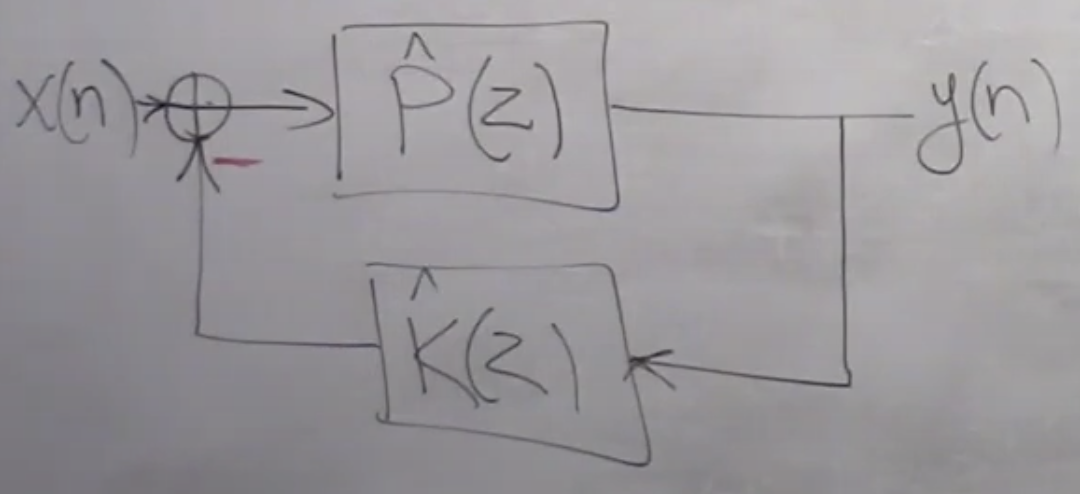
\includegraphics[scale=0.2]{lectures/wk12/img/system.png}
$\implies$
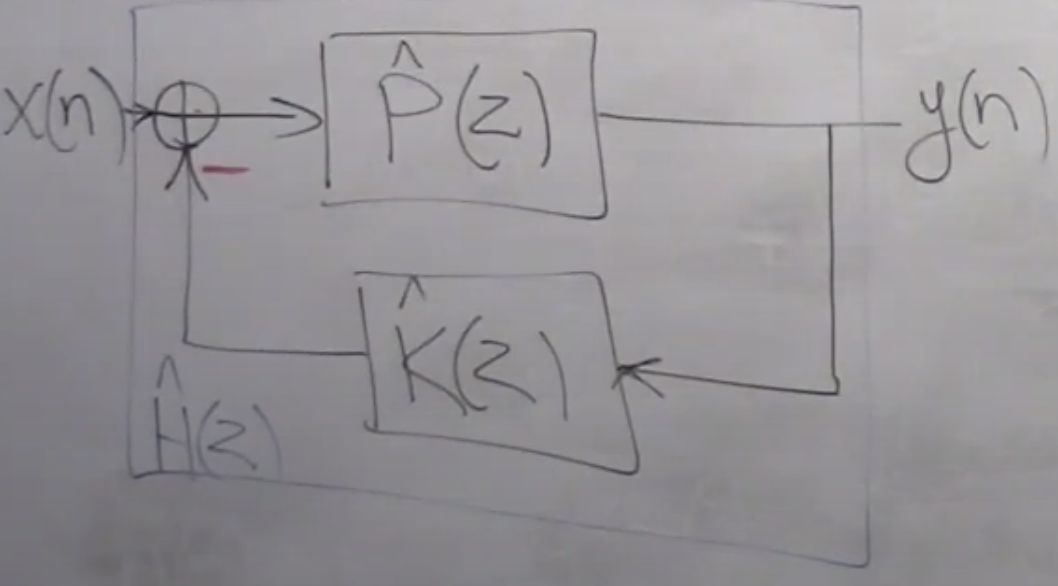
\includegraphics[scale=0.17]{lectures/wk12/img/system2.png}

Reformulating the left system as the right, we can say that $\Hhat=\frac{\hat P(z)}{1+\hat K(z)\hat P(z)}$.

\[
    p(n)=2^n u(n)
\]
is exponential growth so not only is not BIBO stable, but it also does not have a DTFT -- it is faster than polynomial growth.

\begin{align*}
    \hat P(z) 
    &=
    \frac1{1-2\zinv}=\frac{z}{z-2},\ 2<|z|
    &&\text{as }\lambda^n u(n)\zt \frac1{1-\lambda\zinv}=\frac{z}{z-\lambda},\quad|\lambda|<|z|
\end{align*}

\subsection{Shift Register with Gain Factors}
\[
    k(n) = \alpha\delta(n-1)
\]
can be seen as a Shift Register with Gain Factor = $\alpha$.

This signal has the following Z Transform:
\begin{align*}
    \hat K(z) 
    &= \alpha \mathcal Z\{\delta(n-1)\}
    &&\delta(n) \zt \sum_n \delta(n)\zn=1
    \\
    \implies
    \hat K(z) 
    &= \alpha \zinv
    &&\delta(n-1) \zt \sum_n \delta(n-1)\zn=\zinv
    \\
    \implies
    \hat H(z) 
    &= \frac{z}{z-(2-\alpha)}
    \\
    &= \frac{1}{1-(2-\alpha)\zinv}
    \\
    \implies
    h(n)
    &=
    (2-\alpha)^n u(n),\ |2-\alpha|<1.
\end{align*}
with a zero at the origin and a pole at $z=2-\alpha$.

We want $-1<2-\alpha<1$ which is the same as saying $1<\alpha \cap \alpha<3$ or $\boxed{1<\alpha<3}.\hfill\square$


    % \section{Tuesday, November 22th}
\subsection{Steady-State/Transient Response}
Today we will start with one way of splitting the output of a system.\\
Specifically we will split this into a component that persists in time -- steady-state -- and a component that dies out.

Given the following difference equation:
\begin{align*}
    y(n)
    &= \alpha y(n-1) + x(n)\quad|\alpha|<1
    \\
    x(n) &= u(n)\quad\text{System is initially at rest}
    \\
    \Yhat 
    &= \Xhat\Hhat
    \\
    \Yhat 
    &=\alpha z^{-1} \Yhat + \Xhat\implies(1-\alpha z^{-1})\Yhat=\Xhat
    \\
    \Hhat
    &=\frac{\Yhat}{\Xhat}=\frac{1}{1-\alpha z^{-1}}=\frac{z}{z-\alpha},\quad|\alpha|<|z|
    \\
    \Yhat
    &=\frac{z}{z-1}\frac{z}{z-\alpha}
    \\
    &=z\left[\frac{1}{z-1}\frac{z}{z-\alpha}\right]
    =z\left[\frac{z}{(z-1)(z-\alpha)}\right]
    \\
    &= \frac{A}{z-1}+\frac{B}{z-\alpha}
    \\
    &= \underbrace{\frac{1}{1-\alpha}}_{A}\frac{1}{z-1}\underbrace{-\frac{\alpha}{1-\alpha}}_B\frac{1}{z-\alpha}
    \\
    \therefore\Yhat 
    &=z\left[\frac{z}{(z-1)(z-\alpha)}\right]
    \\
    &= {\frac{1}{1-\alpha}}\frac{1}{z-1}{-\frac{\alpha}{1-\alpha}}\frac{1}{z-\alpha},\quad1<|z|
    \\
    &\mathcal Z^{-1}\downarrow
    \\
    y(n)
    &=\underbrace{\frac{1}{1-\alpha}u(n)}_{y_{SS}(n) \text{persists}} - \underbrace{\frac{\alpha}{1-\alpha}\alpha^n u(n)}_{y_{TR}(n)}
    \\
    \lim_{n\to\infty} y_{TR}(n) &= 0
\end{align*}
where we work entirely in the $z$-domain.

The ROC of the system expands outwards from $z=\alpha$ and the unit step has ROC of $1<|z|$ which leads to a non-trivial overlap.

Although we do not see it here, note that a pole/zero cancellation can actually make the ROC of the mixed transform be greater than the minimal intersection.

\begin{shaded}
Q: What's the response of the system to $x(n)=1\quad\forall n\in\mathbb Z$?
\end{shaded}
\textit{Hint:}\[
\beta_{}^n u(n) \zt \frac{1}{1-\beta z^{-1}}, \quad|\beta|<|z|
\]

A: If we plug in $z_0^n=1$ to our system then we get $\Hhat =\frac{z}{z-\alpha},\quad|\alpha|<|z|$ to get output $\frac{1}{1-\alpha}$.

Note that this is the same as $\displaystyle\lim_{n\to\infty} y(n) = \frac{1}{1-\alpha}$.

\hrulefill

\begin{shaded}
What's the response to the input $x(n)=\cos(\omega_0 n)u(n)$?
\end{shaded}
\begin{align*}
    x(n) 
    &=\frac{1}{2} e^{i \omega_0^n} u(n)+\frac{1}{2} e^{-i \omega_0 n} u(n) \\
    \beta^n u(n) \rightarrow \boxed{h(n)=\alpha^n u(n)}& \rightarrow {A \beta^n u(n)}+{B \alpha^n u(n)}
\end{align*}

Everything in this lecture so far has assumed that the system is initially at rest.

\hrulefill

\subsection{Systems not initially at rest}
Given a Causal, BIBO Stable, System. Note that we do not care about the history before the initial state as the initial state tells us all we need to know:
\begin{align*}
    y(n)
    &= \alpha y(n-1)+x(n),\quad|\alpha|<1
    \\
    y(-1)
    &\neq 0;\quad \ x(n)=0,\quad n\ge0
    \\
    y(0)
    &=\alpha y(-1)
    \\
    y(1)
    &=\alpha y(0)=\alpha^2 y(-1)
    \\
    y(2)
    &=\alpha y(1)=\alpha^3 y(-1)
    \\
    \implies
    y_{ZIR}(n)
    &=\alpha^{n+1} y(-1)
    \\
    \text{Now, let } y(-1)
    &=0,\ x(n)=u(n)
    \\
    y_{ZSR}(n)
    &=
    {\frac{1}{1-\alpha}u(n)} - {\frac{\alpha}{1-\alpha}\alpha^n u(n)}
\end{align*}
\begin{shaded}
What's the response if $y(-1)\neq0\quad\&\quad x(n)=u(n)$?
\end{shaded}
\begin{align*}
    y(n)
    &= y_{ZIR}(n) + y_{ZSR}(n)
    \\
    &= \underbrace{\alpha^{n+1}y(-1)}_{y_{ZIR}(n)}
    + \underbrace{\frac{1}{1-\alpha}u(n) - \frac{\alpha}{1-\alpha}\alpha^n u(n)}_{y_{ZSR}(n)}
\end{align*}
\hrulefill
\begin{align*}
    y(n)
    &=
    \alpha y(n-1) + x(n)
    \\
    y(n) u(n)
    &=
    \alpha y(n-1)u(n) + x(n)u(n)
    \\
    \sum_{n=-\infty}^{\infty} y(n) u(n)\zn
    &=
    \alpha \sum_{n=-\infty}^{\infty} y(n-1)u(n)\zn + \sum_{n=-\infty}^{\infty} x(n)u(n)\zn
    \\
    \sum_{n=0}^{\infty} y(n) \zn
    &=
    \alpha \sum_{n=-0}^{\infty} y(n-1)\zn + \sum_{n=0}^{\infty} x(n)\zn
    \\
    \Yhatu
    &=
    \alpha \sum_{n=-0}^{\infty} y(n-1)\zn + \Xhatu
    &&\text{[Unilateral Z Transform]}
    \\
    \text{Lemma: }
    \sum_{n=0}^{\infty} y(n-1) \zn
    &=
    \sum_{m=-1}^{\infty} y(m) z^{-(m+1)}
    = y(-1) + \zinv \Yhatu
    &&\text{[Change of Variables]}
    \\
    &
    &&\text{[$m=n-1\implies n=m+1$]}
    \\
    \hat{y}(z) &=\frac{\alpha y(-1)}{1-\alpha z^{-1}}+\frac{\hat{x}(z)}{1-\alpha z^{-1}} \\
    &=\alpha y(-1) \frac{1}{1-\alpha z^{-1}}+\hat{x}(z) \frac{1}{1-\alpha z^{-1}} \\
    \hat{y}(z) &=\alpha y(-1) \hat{H}(z)+\underbrace{\hat{x}(z) \hat{H}(z)}_{\text{Done Before}}
    \\
    y(n)&= \alpha y(-1)h(n)+
    &&\text{[$h(n)=\alpha^{n}u(n)$]}
    \\
    y(n)&= \alpha y(-1)\alpha^{n}u(n)
    + \frac{1}{1-\alpha}u(n) - \frac{\alpha}{1-\alpha}\alpha^n u(n)
\end{align*}

\subsection{Zero-Input Response/Zero-State Response}
See lecture notes below.

\subsection{Equilization}
See lecture notes below.

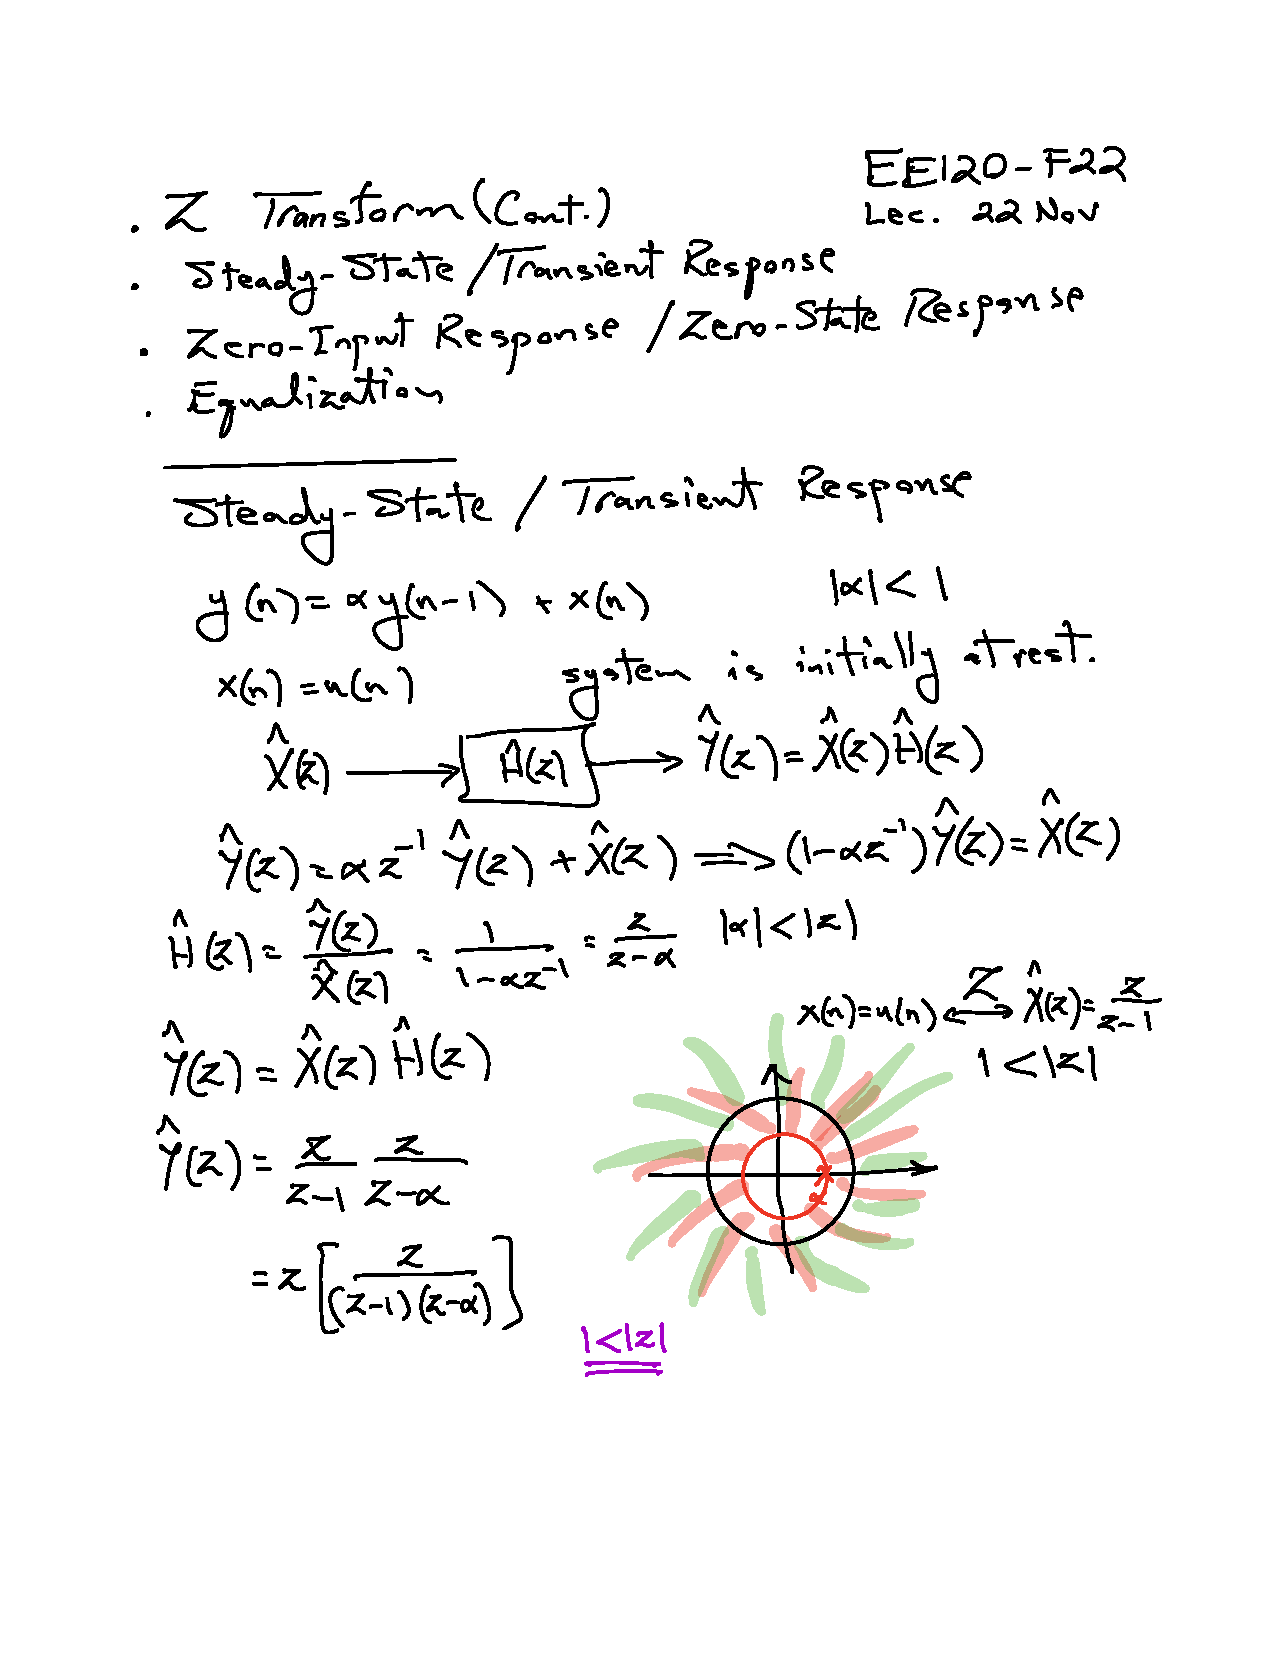
\includepdf[pages=-]{lectures/wk13/EE120-F22-L-2022-11-22-Z-Transform.pdf}

    \section{Appendix}
\subsection{Properties of the DTFT}

\[
    x(n)=\frac{1}{2 \pi} \int_{\langle 2 \pi\rangle} X(\omega) e^{i \omega n} d \omega \longleftrightarrow X(\omega)=\sum_{n=-\infty}^{\infty} x(n) e^{-i \omega n}
\]

\hrulefill

\begin{table}[ht]
  \renewcommand*{\arraystretch}{1.2}
   \centering
  \resizebox{\columnwidth}{!}{
    \begin{tabular}{|c|c|}
    \hline Time domain & Frequency domain \\
        \hline\makecell{$\forall n \in \mathbb{Z}, \quad x(n)$ is real\\\ } & \makecell{$\forall \omega \in \mathbb{R}, \quad X(\omega)=X^*(-\omega)$\\\ } \\
        \hline\makecell{$\forall n \in \mathbb{Z}, \quad x(n)=x^*(-n)$\\\ } & \makecell{$\forall \omega \in \mathbb{R}, \quad X(\omega)$ is real\\\ } \\
        \hline\makecell{\\$\forall n \in \mathbb{Z}, \quad y(n)=x(n-N)$\\\ } 
        & \makecell{\\$\forall \omega \in \mathbb{R}, \quad Y(\omega)=e^{-i \omega N} X(\omega)$\\\ } \\
        \hline\makecell{\\$\forall n \in \mathbb{Z}, \quad y(n)=e^{i \omega_1 n} x(n)$\\\ } 
        & $\forall \omega \in \mathbb{R}, \quad Y(\omega)=X\left(\omega-\omega_1\right)$ \\
        \hline\makecell{\\$\forall n \in \mathbb{Z}$, \\
        $y(n)=\cos \left(\omega_1 n\right) x(n)$\\\ } 
        & \makecell{\\$\forall \omega \in \mathbb{R}$, \\
        $Y(\omega)=\left(X\left(\omega-\omega_1\right)+X\left(\omega+\omega_1\right)\right) / 2$\\\ } \\
        \hline\makecell{\\$\forall n \in \mathbb{Z}$, \\
        $y(n)=\sin \left(\omega_1 n\right) x(n)$\\\ } 
        & \makecell{\\$\forall \omega \in \mathbb{R}$,\\ $Y(\omega)=\left(X\left(\omega-\omega_1\right)-X\left(\omega+\omega_1\right)\right) / {2 i}$\\\ } \\
        \hline\makecell{\\$\forall n \in \mathbb{Z}$, \\ $x(n)=a x_1(n)+b x_2(n)$\\\ } & \makecell{\\$\forall \omega \in \mathbb{R}$ \\ $X(\omega)=a X_1(\omega)+b X_2(\omega)$\\\ }\\
        \hline\makecell{\\$\forall n \in \mathbb{Z}, \quad y(n)=(h * x)(n)$\\\ } & \makecell{\\$\forall \omega \in \mathbb{R}, \quad Y(\omega)=H(\omega) X(\omega)$\\\ } \\
        \hline
        \makecell{$\forall n \in \mathbb{Z}, \quad y(n)=x(n) p(n)$\\\ } & \makecell{\\$\forall \omega \in \mathbb{R}$,\\
        $Y(\omega)=\frac{1}{2 \pi} \int_0^{2 \pi} X(\Omega) P(\omega-\Omega) d \Omega$\\\ }
        \\
        \hline
        \makecell{\\$\forall n \in \mathbb{Z},$\\ 
            $y(n)=$ 
            $\begin{cases}x(n / N) & n \text { is a multiple of } N \\ 0 & \text { otherwise }\end{cases}$
            \\\ 
        }
        & \makecell{$\forall \omega \in \mathbb{Z}$, 
            \\
            $Y(\omega)=X(N \Omega)$
        }
        \\
        \hline
    \end{tabular}
  }
\end{table}

\end{document}
